%%%%%%%%%%%%%%%%%%%%%%%%%%%%%%%%%%%%%%%%%
% Compact Laboratory Book
% LaTeX Template
% Version 1.0 (4/6/12)
%
% This template has been downloaded from:
% http://www.LaTeXTemplates.com
%
% Original author:
% Joan Queralt Gil (http://phobos.xtec.cat/jqueralt) using the labbook class by
% Frank Kuster (http://www.ctan.org/tex-archive/macros/latex/contrib/labbook/)
%
% License:
% CC BY-NC-SA 3.0 (http://creativecommons.org/licenses/by-nc-sa/3.0/)
%
% Important note:
% This template requires the labbook.cls file to be in the same directory as the
% .tex file. The labbook.cls file provides the necessary structure to create the
% lab book.
%
% The \lipsum[#] commands throughout this template generate dummy text
% to fill the template out. These commands should all be removed when 
% writing lab book content.
%
% HOW TO USE THIS TEMPLATE 
% Each day in the lab consists of three main things:
%
% 1. LABDAY: The first thing to put is the \labday{} command with a date in 
% curly brackets, this will make a new section showing that you are working
% on a new day.
%
% 2. EXPERIMENT/SUBEXPERIMENT: Next you need to specify what 
% experiment(s) and subexperiment(s) you are working on with a 
% \experiment{} and \subexperiment{} commands with the experiment 
% shorthand in the curly brackets. The experiment shorthand is defined in the 
% 'DEFINITION OF EXPERIMENTS' section below, this means you can 
% say \experiment{pcr} and the actual text written to the PDF will be what 
% you set the 'pcr' experiment to be. If the experiment is a one off, you can 
% just write it in the bracket without creating a shorthand. Note: if you don't 
% want to have an experiment, just leave this out and it won't be printed.
%
% 3. CONTENT: Following the experiment is the content, i.e. what progress 
% you made on the experiment that day.
%
%%%%%%%%%%%%%%%%%%%%%%%%%%%%%%%%%%%%%%%%%

%----------------------------------------------------------------------------------------
%	PACKAGES AND OTHER DOCUMENT CONFIGURATIONS
%----------------------------------------------------------------------------------------                               
\documentclass[fontsize=11pt, % Document font size
                             paper=a4, % Document paper type
                             twoside, % Shifts odd pages to the left for easier reading when printed, can be changed to oneside
                             captions=tableheading,
                             index=totoc,
                             hyperref]{labbook}
 
\usepackage[bottom=10em]{geometry} % Reduces the whitespace at the bottom of the page so more text can fit

\usepackage[english]{babel} % English language
\usepackage{lipsum} % Used for inserting dummy 'Lorem ipsum' text into the template

\usepackage[utf8]{inputenc} % Uses the utf8 input encoding
\usepackage[T1]{fontenc} % Use 8-bit encoding that has 256 glyphs

\usepackage[osf]{mathpazo} % Palatino as the main font
\linespread{1.05}\selectfont % Palatino needs some extra spacing, here 5% extra
\usepackage[scaled=.88]{beramono} % Bera-Monospace
\usepackage[scaled=.86]{berasans} % Bera Sans-Serif

\usepackage{booktabs,array} % Packages for tables

\usepackage{amsmath} % For typesetting math
\usepackage{graphicx} % Required for including images
\usepackage{etoolbox}
\usepackage[norule]{footmisc} % Removes the horizontal rule from footnotes
\usepackage{lastpage} % Counts the number of pages of the document

\usepackage[dvipsnames]{xcolor}  % Allows the definition of hex colors
\definecolor{titleblue}{rgb}{0.16,0.24,0.64} % Custom color for the title on the title page
\definecolor{linkcolor}{rgb}{0,0,0.42} % Custom color for links - dark blue at the moment

\addtokomafont{title}{\Huge\color{titleblue}} % Titles in custom blue color
\addtokomafont{chapter}{\color{OliveGreen}} % Lab dates in olive green
\addtokomafont{section}{\color{Sepia}} % Sections in sepia
\addtokomafont{pagehead}{\normalfont\sffamily\color{gray}} % Header text in gray and sans serif
\addtokomafont{caption}{\footnotesize\itshape} % Small italic font size for captions
\addtokomafont{captionlabel}{\upshape\bfseries} % Bold for caption labels
\addtokomafont{descriptionlabel}{\rmfamily}
\setcapwidth[r]{10cm} % Right align caption text
\setkomafont{footnote}{\sffamily} % Footnotes in sans serif

\deffootnote[4cm]{4cm}{1em}{\textsuperscript{\thefootnotemark}} % Indent footnotes to line up with text

\DeclareFixedFont{\textcap}{T1}{phv}{bx}{n}{1.5cm} % Font for main title: Helvetica 1.5 cm
\DeclareFixedFont{\textaut}{T1}{phv}{bx}{n}{0.8cm} % Font for author name: Helvetica 0.8 cm

\usepackage[nouppercase,headsepline]{scrpage2} % Provides headers and footers configuration
\pagestyle{scrheadings} % Print the headers and footers on all pages
\clearscrheadfoot % Clean old definitions if they exist

\automark[chapter]{chapter}
\ohead{\headmark} % Prints outer header

\setlength{\headheight}{25pt} % Makes the header take up a bit of extra space for aesthetics
\setheadsepline{.4pt} % Creates a thin rule under the header
\addtokomafont{headsepline}{\color{lightgray}} % Colors the rule under the header light gray

\ofoot[\normalfont\normalcolor{\thepage\ |\  \pageref{LastPage}}]{\normalfont\normalcolor{\thepage\ |\  \pageref{LastPage}}} % Creates an outer footer of: "current page | total pages"

% These lines make it so each new lab day directly follows the previous one i.e. does not start on a new page - comment them out to separate lab days on new pages
\makeatletter
\patchcmd{\addchap}{\if@openright\cleardoublepage\else\clearpage\fi}{\par}{}{}
\makeatother
\renewcommand*{\chapterpagestyle}{scrheadings}

% These lines make it so every figure and equation in the document is numbered consecutively rather than restarting at 1 for each lab day - comment them out to remove this behavior
\usepackage{chngcntr}
\counterwithout{figure}{labday}
\counterwithout{equation}{labday}

% Hyperlink configuration
\usepackage[
    pdfauthor={}, % Your name for the author field in the PDF
    pdftitle={Laboratory Journal}, % PDF title
    pdfsubject={}, % PDF subject
    bookmarksopen=true,
    linktocpage=true,
    urlcolor=linkcolor, % Color of URLs
    citecolor=linkcolor, % Color of citations
    linkcolor=linkcolor, % Color of links to other pages/figures
    backref=page,
    pdfpagelabels=true,
    plainpages=false,
    colorlinks=true, % Turn off all coloring by changing this to false
    bookmarks=true,
    pdfview=FitB]{hyperref}

\usepackage[stretch=10]{microtype} % Slightly tweak font spacing for aesthetics

%\setlength\parindent{0pt} % Uncomment to remove all indentation from paragraphs

\usepackage{mathrsfs, euscript} % Support command like \mathscr
% ***********************************************************
% ******************* PHYSICS HEADER ************************
% ***********************************************************
% Version 2

%-----------------------------------------------------------------------------------------
% Physics Command
%-----------------------------------------------------------------------------------------
%\renewcommand{\labelenumi}{(\alph{enumi})} % Use letters for enumerate
% \DeclareMathOperator{\Sample}{Sample}
\let\vaccent=\v % rename builtin command \v{} to \vaccent{}
\renewcommand{\v}[1]{\ensuremath{\mathbf{#1}}} % for vectors
\newcommand{\gv}[1]{\ensuremath{\mbox{\boldmath$ #1 $}}} 
% for vectors of Greek letters
\newcommand{\uv}[1]{\ensuremath{\mathbf{\hat{#1}}}} % for unit vector
\newcommand{\abs}[1]{\left| #1 \right|} % for absolute value
\newcommand{\avg}[1]{\left< #1 \right>} % for average
\let\underdot=\d % rename builtin command \d{} to \underdot{}
\renewcommand{\d}[2]{\frac{\mathrm{d} #1}{\mathrm{d} #2}} % for derivatives
\newcommand{\dd}[2]{\frac{\mathrm{d}^2 #1}{\mathrm{d} #2^2}} % for double derivatives
\newcommand{\pd}[2]{\frac{\partial #1}{\partial #2}} 
% for partial derivatives
\newcommand{\pdd}[2]{\frac{\partial^2 #1}{\partial #2^2}} 
% for double partial derivatives
\newcommand{\pdc}[3]{\left( \frac{\partial #1}{\partial #2}
 \right)_{#3}} % for thermodynamic partial derivatives
\newcommand{\ket}[1]{\left| #1 \right>} % for Dirac bras
\newcommand{\bra}[1]{\left< #1 \right|} % for Dirac kets
\newcommand{\braket}[2]{\left< #1 \vphantom{#2} \right|
 \left. #2 \vphantom{#1} \right>} % for Dirac brackets
\newcommand{\matrixel}[3]{\left< #1 \vphantom{#2#3} \right|
 #2 \left| #3 \vphantom{#1#2} \right>} % for Dirac matrix elements
\newcommand{\grad}[1]{\gv{\nabla} #1} % for gradient
\let\divsymb=\div % rename builtin command \div to \divsymb
\renewcommand{\div}[1]{\gv{\nabla} \cdot #1} % for divergence
\newcommand{\curl}[1]{\gv{\nabla} \times #1} % for curl
\let\baraccent=\= % rename builtin command \= to \baraccent
\renewcommand{\=}[1]{\stackrel{#1}{=}} % for putting numbers above =
% for operator command
\DeclareMathAlphabet{\mathsfsl}{OT1}{cmss}{m}{sl}
\newcommand{\ope}[1]{\mathsfsl{#1}}
% for commutation operation
\newcommand{\commute}[2]{\left[ #1, #2 \right]}
% for anticommutation operation
\newcommand{\anticom}[2]{\left\{ #1 , #2 \right\} }
% for trace
\newcommand{\Tr}[1]{\mathrm{Tr #1}}

%-----------------------------------------------------------------------------------------
% Physics Command End
%-----------------------------------------------------------------------------------------

% ***********************************************************
% ********************** END HEADER *************************
% ***********************************************************% external physics command support
\graphicspath{{./pic/}}% set for path of pictures
%----------------------------------------------------------------------------------------
%	DEFINITION OF EXPERIMENTS
%----------------------------------------------------------------------------------------

% Template: \newexperiment{<abbrev>}[<short form>]{<long form>}
% <abbrev> is the reference to use later in the .tex file in \experiment{}, the <short form> is only used in the table of contents and running title - it is optional, <long form> is what is printed in the lab book itself

\newexperiment{example}[Example experiment]{This is an example experiment}
\newexperiment{example2}[Example experiment 2]{This is another example experiment}
\newexperiment{example3}[Example experiment 3]{This is yet another example experiment}

\newsubexperiment{subexp_example}[Example sub-experiment]{This is an example sub-experiment}
\newsubexperiment{subexp_example2}[Example sub-experiment 2]{This is another example sub-experiment}
\newsubexperiment{subexp_example3}[Example sub-experiment 3]{This is yet another example sub-experiment}

% Paper List
\newexperiment{Paper000000}[Dynamics of Bose-Einstein condensates in optical lattices]{Dynamics of Bose-Einstein condensates in optical lattices\cite{RevModPhys.78.179}}
\newexperiment{Paper000001}[Intrinsic Dynamical Fluctuation Assisted Symmetry Breaking in Adiabatic Following]{Intrinsic Dynamical Fluctuation Assisted Symmetry Breaking in Adiabatic Following\cite{PhysRevLett.110.130402}}
\newexperiment{Paper000002}[Nonlinear Evolution of Quantum States in the Adiabatic Regime]{Nonlinear Evolution of Quantum States in the Adiabatic Regime\cite{PhysRevLett.90.170404}}
\newexperiment{Paper000003}[Berry phase in nonlinear systems]{Berry phase in nonlinear systems\cite{PhysRevA.81.052112}}
\newexperiment{Paper000004}[Berry phases for the nonlocal Gross–Pitaevskii equation with a quadratic potential]{Berry phases for the nonlocal Gross–Pitaevskii equation with a quadratic potential\cite{0305-4470-39-5-012}}
\newexperiment{Paper000005}[Weakly Nonlinear Time-Adiabatic Theory]{Weakly Nonlinear Time-Adiabatic Theory\cite{Sparber2016}}
\newexperiment{Paper000006}[Theory of nonlinear Landau-Zener tunneling]{Theory of nonlinear Landau-Zener tunneling\cite{PhysRevA.66.023404}}
\newexperiment{Paper000007}[Dynamical fluctuations in classical adiabatic processes: General description and their implications]{Dynamical fluctuations in classical adiabatic processes: General description and their implications\cite{Zhang20121202}}
\newexperiment{Paper000008}[Beyond the geometric phase: intrinsic fluctuation-induced ‘pollutions’ for adiabatic evolution of a nonlinear quantum state]{Beyond the geometric phase: intrinsic fluctuation-induced ‘pollutions’ for adiabatic evolution of a nonlinear quantum state\cite{1751-8121-45-29-295302}}
\newexperiment{Paper000009}[Foundations of Colloid Science - Robert J. Hunter]{Foundations of Colloid Science\cite{Hunter2001}}
\newexperiment{Paper000010}[Electrophoretic mobility of a spherical colloidal particle]{Electrophoretic mobility of a spherical colloidal particle\cite{OBrienWhite1978}}
\newexperiment{Paper000011}[The motion of charged colloidal particles in electric fields]{The motion of charged colloidal particles in electric fields\cite{Teubner1982}}
\newexperiment{Paper000012}[Charged macromolecules in external fields. I. The sphere]{Charged macromolecules in external fields. I. The sphere\cite{Fixman1980}}
\newexperiment{Paper000013}[Geometrical Performance of Self-Phoretic Colloids and Microswimmers]{Geometrical Performance of Self-Phoretic Colloids and Microswimmers\cite{Nourhani2016}}
\newexperiment{Paper000014}[Nano/Microscale motors: biomedical opportunities and challenges]{Nano/Microscale motors: biomedical opportunities and challenges\cite{Wang2012}}
\newexperiment{Paper000015}[Localized Electroosmosis (LEO) Induced by Spherical Colloidal Motors]{Localized Electroosmosis (LEO) Induced by Spherical Colloidal Motors\cite{ChiangVelegol2014}}
\newexperiment{Paper000016}[Electrokinetic Locomotion]{Electrokinetic Locomotion\cite{Moran2013}}
\newexperiment{Paper000017}[Catalytically driven colloidal patterning and transport]{Catalytically driven colloidal patterning and transport\cite{Kline2006}}
\newexperiment{Paper000018}[Self-propulsion of a catalytically active particle near a planar wall: from reflection to sliding and hovering]{Self-propulsion of a catalytically active particle near a planar wall: from reflection to sliding and hovering\cite{Uspal2015}}
\newexperiment{Paper000019}[Understanding the efficiency of autonomous nano- and microscale motors]{Understanding the efficiency of autonomous nano- and microscale motors\cite{Wang2013}}
\newexperiment{Paper000020}[Hierarchical organization of chiral rafts in colloidal membranes]{Hierarchical organization of chiral rafts in colloidal membranes\cite{Sharma2014}}
\newexperiment{Paper000021}[Colloid Transport by Interfacial Forces]{Colloid Transport by Interfacial Forces\cite{Anderson1989}}
\newexperiment{Paper000022}[Phoretic Self-Propulsion]{Phoretic Self-Propulsion\cite{MoranPosner2017}}
\newexperiment{Paper000023}[Anatomy of Nanoscale Propulsion]{Anatomy of Nanoscale Propulsion\cite{Yadav2015}}

%----------------------------------------------------------------------------------------

\begin{document}

%----------------------------------------------------------------------------------------
%	TITLE PAGE
%----------------------------------------------------------------------------------------

\title{\textcap{Research Notes \\[1cm]  
\textaut{\usefont{T1}{phv}{m}{sc} per aspera ad astra }}}

\author{
    \textaut{Yuan Hang}\\ \\ % Your name
}
\date{Date Compiled: \today \\ Data Began: July 11,2016} % No date by default, add \today if you wish to include the publication date

\maketitle % Title page

\printindex
\tableofcontents % Table of contents
\newpage % Start lab look on a new page
\listoffigures % List of figures
\newpage % new page

\begin{addmargin}[4cm]{0cm} % Makes the text width much shorter for a compact look

\pagestyle{scrheadings} % Begin using headers

%----------------------------------------------------------------------------------------
%	LAB BOOK CONTENTS
%----------------------------------------------------------------------------------------
\labday{Wednesday, 13 July 2016}
\experiment{Paper000000}
This review gives pedagogical introduction of Bose-Einstein condensates. It gives some overall background of BEC, especially the experiment realization. It mainly gives that how to realize periodic potential by optical lattice. The theory part starts from the linear case which is very common in condense matter physcis and discuss the beheavior of BEC governed by nonliear schrodinger equation. The techniques used for tackling the nonliear case is analogy to linear case such as weak periodic potential limit and tight-binding limit.
\experiment{Paper000001}
This article discussed the classic adiabatic evolution. In the classic case, the eigenstate in quantum case corresponds to the fixed point of phase space in classic case. So intuitively speaking, the state of classic system could follow the change of fixed point when system is doing adiabatic evolution. The problem comes from possible nonlinearity which could cause bifurcations. In that case, we could not naively apply theorem like quantum adiabatic theorem. In what kind of condition the system could do adiabatic following? This article doesn't answear this question. However, it proposed that the intrisic dynamical fluctuation could be used to determine the direction of bifurcation and disccuss the berry phase in cyclic adiabatic evolution case.
\experiment{Summary}
Thouless Pumping shows that the quantizaiton of particle transport  under cyclic adiabatic pumping. The problem I want to investigate is the case of nonlinear schrodinger equation. The numerical simulation shows that the pumping is still quantized even adding the nonlinear interaction term as long as the nonlinear effect is not so strong. How to prove the quantization in nonlinear situation? Compare with linear case, Thouless apply the adiabatic perturbation theory to first order. It shows that the charge pumping could be expressed as integration of Berry curvature. What about the nonlinear situation? I need to consider the adiabatic perturbation theory in nonlinear case. Then I expect that the charge pumping in nonlinear case still could be expressed into something like Berry curvation as long as the topology of band structure is not significantly changed.\\
The adiabatic perturbation theory for nonlinear system is absent. I want to find a way out from classic mechanics. I want to investigate the canonical perturbation theory in classic menchanics and see how the adiabatic theorem is developed in classic limit. Hope to find some inspirations.
\labday{Thursday, 14 July 2016}
To do list:
\begin{enumerate}
\item
Learn Classic Mechanic Method.
\begin{enumerate}
\item
Hamilton-Jacobi Theory Checked.
\begin{equation}
\pd{S(q,\alpha,t)}{t}+H(q,\pd{S}{q},t)=0
\end{equation}
\item
Action-Angle Variables Checked.
\begin{equation}
J=\oint p\mathrm{d}q
\end{equation}
\begin{equation}
\omega=vt+\beta
\end{equation}
\begin{equation}
\Delta \omega =\oint \pd{\omega}{q}\mathrm{d}q=1=v\tau
\end{equation}
\item
Canonical Perturbation Theory Checked.
\begin{equation}
H(q,p,t)=H_0(q,p,t)+\Delta H(q,p,t)
\end{equation}
\begin{equation}
\left\{
\begin{aligned}
\dot{\alpha_i}&=-\pd{\Delta H(\alpha,\beta,t)}{\beta_i}\\
\dot{\beta_i}&=\pd{\Delta H(\alpha,\beta,t)}{\alpha_i}
\end{aligned}
\right.
\end{equation}
\item
Classic Adiabatic Theorem - Adiabatic Invriant
The action variables $J$ plays the role of adiabatic invriant. 
\begin{equation}
\bar{\dot{J_0}}=0+O(\dot{a}^2,\ddot{a})
\end{equation}
\end{enumerate}
\end{enumerate}
%----------------------------------------------------------------------------------------
\labday{Friday, 15 July 2016}
To do list:
\begin{enumerate}
\item
Classic correspondence of nonlinear schrodinger equation
\item
Find a simple model system of nonlinear schrodinger equation
\item
Try to apply canonical perturbation theory to find the adiabatic evolution of the eigenstate of the model system
\end{enumerate}
\experiment{Paper000002}
This paper try to generalize the adiabatic theorem to systems governed by  nonlinear schrodinger equaiton. The key approach used in this paper is to convert nonlinear schrodinger equation into an equivalent classic hamiltonian describtion. The eigenstate in quantum sense then corresponds to a fixed point in phase space of hamitonian dynamics. Thus, it claims that usually we chould expect adiabatic following holds for elliptical fixed point while for hyperbolic fixed point is not. \\
This paper also find a connection between classic adiabatic invirant- action variables and AA phase. It shows that the AA phase plays the role of adiabatic invriants in the nonlinear system as long as the nonlinearity in not too strong(no significant tunnuelling).
%----------------------------------------------------------------------------------------
\labday{Monday, 18 July 2016}
\experiment{Paper000003}
I don't quite understand the main idea of this paper. This paper proposed a possible definition of nonlinear berry phase. Beside the uausal term in linear case, there is an additional term caused by nonliear effect. The author write in the abstract explains as'' the Bogoliubov excitations around the eigenstates are found to be accumulated during the nonlinear adiabatic evolution and contribute a finite phase of geometric nature''.

\experiment{Paper000004}
This paper gives the exact solution of GP equation in the sense of order $1/T$. The content of this paper is pretty technical. In my opinion, the core aspects of the approximation method used in this paper is in two aspects. First, it associated the solution of nonliear GP equation with the ``classical'' Ehrenfest equation; Second, it linearizes the nonliear GP equation around the mean value of operators. The details of this paper is really disgusting... I can't go throught the whole content. However, it least provides me a possible way to find the adiabatic perturbation in nonlinear system. The result of this paper shows that we should expect that there exists some additional terms caused by nonlinearity compared with the linear case. 
%----------------------------------------------------------------------------------------
\labday{Tuesday, 19 July 2016}
\experiment{Paper000005}
%----------------------------------------------------------------------------------------
\labday{Wednesday, 20 July 2016}
To do list:
\begin{enumerate}
\item
Study the theory of nonlinear Landau-Zener Tunnelling thoroughly.
\item
Do numerical calculation of nonliear Schrodinger equation
\item
Do numerical calculation of corresponding classic hamitonian system
\end{enumerate}
\experiment{Paper000006}
This paper give a thorough description of nonliear Laudan-Zener tunneling. The hamiltonian is a simple two level system with its eigenenergy affected by eigenstate population. Nonliearity always gives us troubles but also richer structures. This paper maps the nonlinear two level system to an effective classical system. Choose the action-angle as the canonical coordinations and use the evolution of fixed point in phase space to discuss the phenomena of tunnelling. \\
The focus of this paper is to used these classic methods to calculate the tunnelling probability. This is not the problem I care about. I want to extend 1st order adiabatic perturbation theory to nonlinear region. However, as a simple model system, it's really useful to learn this model no matter for inspiration or verification.\\

%----------------------------------------------------------------------------------------
\labday{Thursday, 21 July 2016}
To do list:
\begin{enumerate}
\item
Numerical calculation of two level Landau-Zener model
\item
Learn adiabatic perturbation theory in classic mechanics
\end{enumerate}
Unfinished. To be continued tommorrow.
%----------------------------------------------------------------------------------------
\labday{Friday, 22 July 2016}
The same as yesterday. Numerical calculation of two-level Landau-Zener model finished.
%----------------------------------------------------------------------------------------
\labday{Monday, 25 July 2016}
\experiment{Paper000007}
This paper gives a general description of classical adiabatic evolution. It discussed the time evolution of the so-called Intrinsic Dynamical Fluctuation during the adiabatic process. Put it simply, it derives the time evolution of the deviation from ideal classical adiabatic orbits. The general result is not a very simple form and not easy to calculate. However, authors also provide some simple cases for verification. One is for the fixed-point solution which could simplify the general result. The another one is for two-mode GP equation. It serves as an example to discuss the possible ``pollution'' to Hannay angle in classic adiabatic process. In principle, the method used in this paper could regard as a first order adiabatic perturbation theory. I think it will be useful for my disccusion of interband effect in nonlinear region.
%----------------------------------------------------------------------------------------
\labday{Tuesday, 26 July 2016}
\experiment{Paper000008}
This paper discusses the emergence of ``pollution'' terms to geometric phase arising in general adiabatic evolution. This paper is based on the previous paper\cite{Zhang20121202} which gives a description of intrinsic dynamical fluctuations. This paper shows that the overall phase of general quantum state in two-level GP equation consists of five terms:
\begin{equation}
\phi=I_0\Delta \theta + \beta_{Berry}+D_0+\Theta_{pol}+D_{pol}
\end{equation}
Besides the expected berry phase term, $D_0$ is the new dynamical phase which is the analogy to linear case; $I_0\Delta \theta$ will vanish for eigenstate; $\Theta_{pol}$ and $D_{pol}$ are ``pollution'' caused by intrinsic dynamical fluctuation. It depends on the details of adiabatic control.\\
Adiabatic theorem for general quantum state in GP equation is not well described yet. Maybe it's helpful to take a look at it.
%----------------------------------------------------------------------------------------
\labday{Wednesday, 27 July 2016}
To do list:
\begin{enumerate}
\item Do numerical simulation of Two-Mode GP equation based on classic Hamiltonian method for further investigation.
\item Consider the case of adiabatic evolution for general quantum state.
\end{enumerate}
Unfortunately, unsually ODE numerical method is not stable. The corresponding classic Hamitonian dynamical equations have singular around the eigenstates. The Runge-kutta likewise method cannot maintain the norm of the state which is impossed as constraint during the derivation. This shortage makes result breaks down quickly. Therefore, This way is not appropriate for simulating adiabatic process (long time evolution is needed). The next attempt, I will use time splitting method directly from schr$\ddot{o}$dinger equation. Hope it works well.

\labday{Thursday, 28 July 2016}
To do list:
\begin{enumerate}
\item
Try to accomplish numerical simulation of Two-Mode GP equation. Note to void numerical instability caused by nonliearity.
\item
Check some result in theory.
\end{enumerate}
\labday{Tuesday, 2 August 2016}
I meet problems in numerical calculation. I can't even get a self consistent eigenstate of Two-Mode GP equation!!!! In order to obtain the eigenstate of Two-Mode GP equation, I find that the components of eigenstate must satisfy following three conditions simultaneously:
\begin{equation}
\begin{aligned}
\abs{b}^2-\abs{a}^2&=-\frac{1}{\epsilon}\left(\frac{\gamma}{2}+\frac{C}{2}\right)\\
\abs{b}^2+\abs{a}^2&=1\\
-\frac{2}{V}\left[\frac{\gamma}{2}+\frac{C}{2}(\abs{b}^2-\abs{a}^2)-\epsilon\right]a&=b
\end{aligned}
\end{equation}
The most tricky problem is that I find these three conditions cannot be satistied simultaneously!!!!!!  which leads that I cannot get a self-consistent solution! I need to check further and decide whether all these three conditions are necessary or if there is something wrong during my derivation. Time is limited, be quick!
\labday{Friday, 5 August 2016}
Ok, I have to admit that all the problems are caused by my stupid mistake. I write the relation of population difference incorrectly... Finally, the numerical simulation of Two-Mode GP equation is finished. The simulation results are pretty good but still need more understanding. \\
Next step, I will try to add nonlinearity into usual Chern insulator and calculate some properties of it, especially the adiabatic pumping. Hope the time is still enough, come on!
To do list of recent days:
\begin{enumerate}
\item
Be familiar with the Chern insulator.\\
After reading about some materials about topological insulator, I begin to have some feelings about the concept of topological insulator. My study starts from Su-Schrieffer-Heager(SSH) model to Rice-Mele model( + onsite potential) and finally to the simplest 2D Chern insulator. I also learn a little about the edge-bulk correspondce and how symmetry plays an important role in such a relation.
\item
Consider how to add nonliearity into original model or establish relation with Two-Mode GP equation.\\
I tried to add a diagonal on-cell state-dependent interaction to the Chern insulator. However, this model has difficulties caused by intercell interaction which makes the equation coupled with each other. I am still making an effort to solve this model or try other ways of introducing nonliearity.
\item
Be familiar with the calculation of adiabatic pumping\\
About the adiabatic pumping, the traditional way is based on the first order adiabatic perturbation theory. The calculation needs the time evolution of state. The linear case connects the state time evolution besides the adiabatic theorem claims with the berry curvature and then leads to the quantization of adiabatic pumping. A severe problem of adiabatic pumping in the nonlinear case is that there is not first order adiabatic perturbation theory. Until now, I begin to doubt that whether I should use adiabatic perturbation theory to handle this problem. Although I admit that there perhaps exist appropriate perturbation theory at least in weak nonliearity case, I still wonder that there may have other better views to think of this problem.\\
By the way, we usually do calculation with floquet state when system possess translational symmetry. Sometimes using Wannier state instead may give us a better illustration.
\item
Try to find clues about how to do first order adiabatic perturbation with nonliearity, this would be difficult.\\
Still no idea...
\end{enumerate}
\labday{Wednesday, 31 August 2016}
Recently, I begin to prepare some necessary background of graduation design. My graduation design will be related to Janus particle and mainly about the self-electrophoresis. In order to be prepared to enter this field, I need to pick up my knowledge about the fluid mechanics and electrodynamics firstly and be familiar with some essential concepts of this field. After skimming several papers in this field, my arrangement of preparation is as following:
\begin{enumerate}
\item
Chapter 4, Chapter 7 and Chapter 8 of \emph{Foundations of Colloid Science} by Robert J. Hunter.
\item
Basic theory of modeling the motion of charged colloidal under exteral electric field.
\item
Basic theory of modeling the motion of charged Janus particle under self-generated electric field.
\end{enumerate}
\experiment{Paper000009}
\experiment{Paper000010}
\experiment{Paper000011}

\labday{Wednesday, 7 September 2016}
\experiment{Summary of NUS summer research program}
\emph{Intro.}:\\

Before I depart from NUS and finish my summer research program in NUS, I want to do a brief summay of research during these two months. Although I feel a little regret that I can't obtain any results during this summer research program, I don't want my efforts disappeared in my memory. This short article is used for recording the road map of this summer research and hope it could be served as a good experience for my future research.\\

\emph{Some informations}:\\

Name of Program: IRO Summer Research Program, National University of Singapore\\
Start and End Date of Program: 27-JUNE-2016 to 9-SEPT-2016\\
Student No.: A0151581J\\

\emph{The start of my summary}:

Before I start my summer research program, my focus is mainly put on the geometry phase and adiabatic perturbatino theory. \\

My basic concepts of geometry phase are established by reading the review paper \emph{Berry phase effects on electronic properties}\cite{XiaoChangNiu2010} and the notes \emph{Geometry and Topology  in Electronic Structure Thoery}\cite{Resta2016}. Throught reading these materials, I know how to define Berry phase and Berry curvature and many applications where geometry phase emerged, such as A-B effect, polarization, quantization of transport, Chern insulator and correction to the semiclass equaiton of motion in condense matter physics and so on. It shows that the geometry phase really has promising applications in many fields of physics. \\

On the other hand, I also learned some basic techniques of adiabatic perturbation theory. The start point of this is the common adiabatic theorem in quantum physics which states that if the initial state of a system is the eigen-energy state then the system will stay at the instantaneous eigen-state as long as the parameters changed slowly enough (adiabatic evolution) apart from a dynamical phase and a geometrical phase will emerge. \\

Then, When I arrived in NUS and Prof. Gong wants me to study the interband coherence effect of systems which are governed by Gross–Pitaevskii equation(Nonlinear schr$\ddot{o}$dinger equation). At the beginning, I am ambitious and I don't think this is a very tough problem. Then I quickly learnd the interband coherence effect in linear case \cite{PhysRevB.91.085420}, i.e. the evolution of system is still governed by schr$\ddot{o}$dinger equation. Put it simply, the usually adiabatic theorem only concerned about the time evolution of energy eigenstate while the interband coherence effect will occur when we consider the superposed initial state. The first order adiabatic perturbation theory will give the term which is proportional to the inverse of time $T$, i.e.
\begin{equation}
C_n(t)=C_n(0)+f\times\frac{1}{T}+O(\frac{1}{T^2})
\end{equation}
In common adiabatic theorem, we could safely eliminate the first order term as the term $T$ approaches to infinity. However, when we consider some special quantities (for example the displacement of wannier state in the paper\cite{PhysRevB.91.085420}), the first order correction combined with the infinite long time integration will produce a zeroth order correction:

\begin{equation}
\begin{aligned}
\Delta\avg{x}&=\sum_n\int \mathrm{d}k \int \mathrm{d}\beta B_n(\beta,k)\rho_{n,k}(0)\\
&-2\sum_{m\neq n}\int \mathrm{d}k \left[C^\ast_{n,k}(0)C_{m,k}(0)\frac{\mathrm{d} E_{n,k} }{\mathrm{d} k}W_{nm,k}(0)\right]
\end{aligned}
\end{equation}
where the first term is the common integration of Berry curvature $B_n(\beta,k)$ but weighted by the initial population. The second term is the additional term induced by interband coherence and is sensitive to the detail of adiabatic protocol.\\
It shows that it's a significant correction which cannot be ignored even in the adiabatic limit and which depends on the initial state and the rate of parameters changing.\\

I want to reproduce similar result in systems governed by GP equation. Look at the whole derivation process in linear system, the key is the first order adiabatic perturbation theory. If we could obtain the first order adiabatic evolution of state, then we could easily calculate our concerned quantities, such as the adiabatic pumping or displacement.  Take the diabatic pumping as an example. The typical Thouless pumping is given by\cite{PhysRevB.27.6083}:
\begin{equation}
Q=\frac{1}{2\pi}\int_{-\pi}^{\pi}\mathrm{d}k \int_0^T \mathrm{d}t \bra{\Psi(t)}\pd{H(k,t)}{k}\ket{\Psi(t)}
\end{equation}
With the aid of aidabatic perturbation theory, in common linear system, we could prove that the number of charge pumping in each periodic cycle could be expressed as the integration of Berry curvature and that shows the the number particle pumping is quantized and is exactly the Chern number of corresponding band.\\

The problem is that there is no developed adiabatic perturbation theory for nonlinear system. Then, I try to find the appropriate mathematical techniques to handle this difficulty. The first attempt is related to the so-called nonlinear adiabatic theorem\cite{PhysRevLett.90.170404,PhysRevA.81.052112}. In the paper \cite{PhysRevLett.90.170404}, authors use the ``classic'' form of nonlinear Schr$\ddot{o}$dinger equation to discuss the adiabatic theorem:
\begin{equation}
i\d{\psi_j}{t}=\pd{}{\psi_j^\ast}\mathbb{H}(\psi,\psi^\ast,\v R)
\end{equation}
Choose a specific set of canonical variables which are called action-angle in classic mechanics, the above form could be written equivalently as:
\begin{equation}
\left\{
\begin{aligned}
\d{q_j}{t}&=\pd{H}{p_j}\\
\d{p_j}{t}&=-\pd{H}{q_j}
\end{aligned}
\right.
\end{equation}
where
\begin{equation}
\left\{
\begin{aligned}
q_j&=\mathrm{arg}\psi_j - \mathrm{arg} \psi_N\\
p_j&=\abs{\psi_j}^2\\
q_N&=\mathrm{arg} \psi_N\\
p_N&=\sum_{j=1}^N \abs{\psi_j}^2
\end{aligned}
\right.
\end{equation}
Because of the conservation of probability, the overall phase could be seperated out from the Hamiltonian and the time-evolution of overall phase is given by a seperated equation:
\begin{equation}
\d{\lambda(t)}{t}=\sum_{j=1}^N \phi_j^\ast i \pd{}{t}\phi_j - \sum_{j=1}^N \phi_j^\ast \pd{}{\phi_j^\ast}H
\end{equation}
The second term is the usually time integration of energy in linear case which is corresponded to the dynamical phase part; The first term could still be regarded as a certain kind of Berry phase in nonlinear case\cite{PhysRevA.81.052112}. \\

After mapping the quantum system to canonical classic system, the eigenstate maps to the fixed point in phase space of canonical system. To further understand the aidabatic theorem in nonlinear system, I choose the simplest system two-level system-Landau-Zener system to illustrate the nonlinear adiabatic theorem\cite{PhysRevA.66.023404}. In this paper \cite{PhysRevA.66.023404}, authors showed clearly the band-structure of Landau-Zener model and applied the above mentioned action-angle techniques to show the adiabatic theorem and calculate the tunnelling rate. It also discussed the conditions for adiabatic theorem holds in nonlinear case.\\

To sum up, nonlinearity will cause the emergence of loop structure in energy specturm and system will have number of eigen-state beyond their physical dimension. The adiabatic theorem will usually break down when passing through the loop structure caused by nonlinearity. \\
According to the classic adiabatic theorem, the action $I$ could serve as the adiabatic invariant and will remain constant during adiabatic change. Thus, for a system initially prepared at the energy eigen-state, we expect the system evolves along the fixed point in each time steps. The problem comes when the fixed point collided with a saddle point in the phase space. After passing throught this transition point, action $I$ will still remain constant because of adiabatic control but maybe a different constant compared with original action. That's why tunnel happens even in adiabatic limit.\\

Above readings and discussions didn't give me much useful information to solve my problem. Because above mentioned nonlinear adiabatic theorem only concerned the zeroth order approximation, I want the first order correction of adiabatic evolution to obtain some undiscoverd results. Fortunately, this problem is concerned in paper \cite{PhysRevLett.110.130402, 1367-2630-16-12-123024, 1751-8121-45-29-295302, Zhang20121202}. Let me summarize the main ideas I learnt from these papers here:

The paper \cite{PhysRevLett.110.130402} focused on the first order correction upon the adiabatic theorem which is called intrinsic dynamical fluctuation in that paper. It shows that such kind of fluctuation around the ideal adiabatic evolution must exist and could be useful for determining the direction of bifurcation which is usually regarded as indeterministic at least in my opinion. \\

The detailed calculation of intrinsic dynamical fluctuation is given in the paper \cite{Zhang20121202}. Sitll utilize the action-angle variables, the evolution of system could be expressed as:
\begin{equation}
\left\{
\begin{aligned}
\d{I_i}{t}&=-\pd{\v W}{\theta_i}\d{\v R}{t}\\
\d{\theta_i}{t}&=\omega_i(\v I;\v R)+\pd{\v W}{I_i}\d{\v R}{t}
\end{aligned}
\right.
\end{equation}
where
\begin{equation}
\omega_i(\v I,\v R)=\pd{H}{I_i}
\end{equation}
is the angular frequency and $\v W$ is defined as
\begin{equation}
\v W=\nabla_{\v R} F[\v I,\v q(\v I,\gv \Theta,\v R),\v R]-\v p \cdot \nabla_{\v R}\v q(\v I,\gv \Theta,\v R)
\end{equation}
Define the $\bar{\v I}$ and $\bar{\v \Theta}$ as idealized trajectory of adiabatic evolution, then
\begin{equation}
\left\{
\begin{aligned}
\v I&=\bar{\v I}+\delta \v I\\
\gv \Theta&=\bar{\gv \Theta}+\delta \v \Theta
\end{aligned}
\right.
\end{equation}
Keep up to first order of $\delta \v I$ and $\delta \v \Theta$, following differential equation is given:
\begin{equation}
\Gamma
\begin{pmatrix}
\delta \v p\\
\delta \v q
\end{pmatrix}
=
\gv \Sigma \cdot \d{\v R}{t} + \Pi 
\begin{pmatrix}
\delta I_1\\
\delta I_2\\
\vdots\\
\delta I_N
\end{pmatrix}
+
\begin{pmatrix}
\pd{\delta \v p}{\bar{\theta_j}}\omega_j\\
\pd{\delta \v q}{\bar{\theta_j}}\omega_j
\end{pmatrix}
\end{equation}
Details could be found in paper \cite{Zhang20121202}. This is a complicated differential equation and it's hard to apply to the system I want to study. The complicated form really bothers me a lot but at least I finally have a seeming possible tool to calculate the first order fluctuation upon the zeroth order adiabtatic evolution.\\

Although the possible tool is complicated and hard to apply, I still have hopes to solve my target problem. Then, I turn my attention to the specific systems. I choose the Chern insulator as my model system and try to add nonlinearity into Chern insulator. I try to discuss the pumping of Chern insulator and stability of edge mode with the nonlinear on-site potential. In order to achive that, I study the basic concepts of topological insulators. My main reference in this stage is a book named \emph{A Short Course to Topological Insulator} \cite{JanosK.Asboth2016}. I start from the Su-Schrieffer-Heeger(SSH) Model to Rice-Mele Model with on-site potential additionally and finally to the Qi-Wu-Zhang model which is the simplest Chern insulator I want to study. Besides the main line of study, I want know about the bulk-edge correspondce which I think it has special interest. The number of the possible edge mode is related to the properties of bulk such as the Chern number. The existence of edge mode is also closely related to the symmetry which system broken. \\

The next enters my concrete model I used. The Hamiltonian of Chern insulator in momentum space could be written as:
\begin{equation}
\tilde{H}(k_x,k_y)=\sin(k_x)\sigma_x+\sin(k_y)\sigma_y+\left[M+\cos(k_x)+\cos(k_y)\right]\sigma_z
\end{equation}
The Hamiltonian in real space is
\begin{equation}
\begin{aligned}
H&=\sum_{\v r} \left[C^\dagger_{\v r}\frac{-i\sigma_x-\sigma_z}{2}C_{\v r+\uv x} + C^\dagger_{\v r}\frac{i\sigma_x-\sigma_z}{2}C_{\v r-\uv x} \right. \\
&\left.+ C^\dagger_{\v r}\frac{-i\sigma_y-\sigma_z}{2}C_{\v r+\uv y} + C^\dagger_{\v r}\frac{i\sigma_y-\sigma_z}{2}\sigma_{\v r-\uv y}-mC_{\v r}^\dagger C_{\v r}\right]
\end{aligned}
\end{equation}
In order to see the edge mode, choose the y-direction to be periodic and transform it to momentum space and keep x-direction in real space:
\begin{equation}
\begin{aligned}
H_0(k_y,x)&=\sum_{k_y}\sum_x \left\{ C_{x,k_y}^\dagger \frac{-i\sigma_x-\sigma_z}{2} C_{x+\uv x,k_y}\right.\\
&+C^\dagger_{x,k_y}\frac{i\sigma_x-\sigma_z}{2}C_{x-\uv x,  k_y}\\
&\left. +\left[\sin k_y \sigma_y + (2-m-\cos k_y)\sigma_z\right]C_{x,k_y}^\dagger C_{x,k_y}\right\}
\end{aligned}
\end{equation}
Now, I want to  add nonlineartiy into the on-site potential. I imitate to add the nonlinearity which lets the on-site potential depends on the population difference in each sublattice:
\begin{equation}
H_N(k_y,x)=\sum_{k_y}\sum_x g(\abs{b_x}^2-\abs{a_x}^2)\sigma_z C^\dagger_{x,k_y}C_{x,k_y}
\end{equation}
where $g$ controls the strength of nonlinearity and $\abs{a_x}^2$ and $\abs{b_x}^2$ are the population on sublattice A and B in cell x respectively. Therefore, the Hamiltonian in matrix form is:
\begin{equation}
H=
\begin{pmatrix}
H_{11}&H_{12}&\cdots\\
H_{21}&H_{22}&\cdots\\
\vdots&\vdots&\ddots
\end{pmatrix}
\end{equation}
where
\begin{equation}
H_{11}=
\begin{pmatrix}
2-m-\cos k_y + g(\abs{b_1}^2-\abs{a_1}^2)& -i\sin k_y\\
i\sin k_y&-(2-m-\cos k_y)-g(\abs{b_1}^2-\abs{a_1}^2)\\
\end{pmatrix}
\end{equation}
\begin{equation}
H_{12}=
\begin{pmatrix}
-\frac{1}{2}&-\frac{1}{2}i\\
-\frac{1}{2}i&\frac{1}{2}
\end{pmatrix}
\end{equation}
\begin{equation}
H_{21}
\begin{pmatrix}
-\frac{1}{2}&\frac{1}{2}i\\
\frac{1}{2}i&\frac{1}{2}
\end{pmatrix}
\end{equation}
\begin{equation}
H_{22}=
\begin{pmatrix}
2-m-\cos k_y + g(\abs{b_2}^2-\abs{a_2}^2)& -i\sin k_y\\
i\sin k_y&-(2-m-\cos k_y)-g(\abs{b_2}^2-\abs{a_2}^2)\\
\end{pmatrix}
\end{equation}

The eigen-energy is given by:
\begin{equation}
H \Psi=\epsilon \Psi
\end{equation}
However, the coupling caused by intercell hoping made this problem is hard to solve. I try to suppress the intercell hoping firstly, then the eigenenergy in each unicell is just like in the Landau-Zenner case. The eigen-energy when intercell hoping is suppressed is given as:
\begin{equation}
\epsilon^4+(2C_i g)\epsilon^3+(C_i^2 g^2 -W^2+sin^2k_y)\epsilon^2+(2C_i g \sin^2k_y)\epsilon + C_i^2g^2\sin^2k_y=0
\end{equation}
where $g$ is the strength of nonliearity, 
\begin{equation}
\begin{aligned}
C_i&=\abs{a_i}^2+\abs{b_i}^2\\
1&=\sum_i C_i\\
W&=2-m-\cos k_y\\
\abs{b_i}^2-\abs{a_i}^2&=-\frac{W(\abs{a_i}^2+\abs{b_i}^2)}{g(\abs{a_i}^2+\abs{b_i}^2)+\epsilon}
\end{aligned}
\end{equation}
Suppose the $\gamma$ is used for controling the strength of intercell hoping. Then I aidabatically open the intercell hoping $\gamma$ from $0$ to $1$. Thus, a initial eigenstate will evolve as the instantaneous eigenstate as long as the adiabatic theorem holds. I will use this to calculate the energy-specturm of the coupled situation and check the stability of edge-state.

\labday{Monday, 19 September 2016}
\experiment{The beginning of my thesis}
After tackling some meticulous affairs, now I am ready to switch myself into research mode. I have to catch up quickly then try to think about the problem in my own point of view. The main task of week is to read some background papers\cite{ChiangVelegol2014,Fixman1980,Kline2006,OBrienWhite1978,RobertJ.HunterRowell1981,Teubner1982} about Janus particle which I have read before. However, this time I need to read carefully and understand the detail of each paper. Hope you well in the next coming year!

\labday{Tuesday, 22 September 2016}
\experiment{Three Talks given by Peter H{\"a}nggi}
What a coincidence could meet with Peter H{\"a}nggi again in my university. During my visit in NUS, Peter collaborated with Deng Jiawen to write a paper about Jarzynski equality\cite{Jarzynski1997}. The central idea of their work is pretty simple and straightforward. They want to illustrate a case which the ensemble average of exponential work in Jarzynski equality will be divergent even in adiabatic limit. Then, the ensemble average of exponential work will be divergent for all processes( include non-adiabatic processes). They showed this situation in classic case and verified it with numerical examples. That's all I want to recall about Peter in singapore. \\
This time in my university, Peter gave a talk about Brownian motion in Zhiyuan Salon and another two talks about diffusion in confined geometry \cite{burada2009diffusion} for Zhang Hepeng's group. The talk given in Zhiyuan Salon is pretty general and I didn't get too much in this talk. Thus, I mainly want to record something I learnt from last two talks.\\
To describe the motion of small particles in fluid, the most straightforward idea is to solve the equations of motion of all particles in the system. However, that's too complicated to solve. In order to simplify the problem, a random noise could be added to the equation of motion to replace the coupling with external environment. That's the view of Langevin. This idea is still Newton-like and the trace of single particle is crucial in this theory. On the contrary, the idea of Fork-Plank thoery gave up the idea to trace each particle individually. The Fork-Plank equation cares about the possiblity. These two ideas are equivalent.\\
Peter mainly focused on the diffusion in confined geometry during these two talks. From my point of view, the mathematics involved in this problem is not very difficult. Just solve the Fock-plank equation with confined boundary conditions. Maybe it is not easy to solve. Then apply some approximation method and check the validity of this approximation. If the approximation is valid, then derived the relevant properties in this situation such diffusion constant or mobility. Perhaps, we check the theory proposed by Peter using numerical tools and then do some modifications. At last, we could check the theory via experimental method. It's a pretty prospective road map. \\
To sum up, I have some interests about this problem and maybe I could talk about it further with Yang Xiang and Ding Ziwei in later group meeting. If possible, I am also willing to participate in this problem.

\labday{Wednesday, 28 September 2016}
\experiment{First Associated Group Meeting of Soft Matter, 2016 Autumn}
Successfully finishing the meeting in Harbin, I finially could find some time to do my own work. Today's associated group meeting is about the Man-made particles self-assemble like atoms. The fabrication process of this kind of man-made particle is pretty interesting. Professors are also debating fervently about the details of the fabrication techniques. However, the long time needed for assembling is not good for application and I also don't expect such a man-made particles to form a macroscopic structure. No matter what, it provides a method to fabricate particles which could form atoms with certain symmetry. I am looking forward to the next group meeting. \\
Prof. Xing said he will use two hours to give a talk about the book Life-As a matter of fat in the next group meeting. And I heard Mr. Liang Yihao is pretty good at GPU computation. That's pretty interesting and maybe I could find a chance to talk with him. 
\labday{Thursday, 2 October 2016}
After the talk with Liu Chang, now I have got a general idea about the COMSOL model already established. The model could generally be divided into two part: One is for electrostatic interactions, another is for hydrodynamic interactions. A pretty special point is that Liu told me that there is no consideration of ions in this model. The reasons are given by the works of Velegol\cite{Kline2006,ChiangVelegol2014}. It seems that Velegol absorbed the ionic flux into the boundary conditions. I will read these paper carefully later.\\
Besides, the model used a somewhat unfamiliar boundary condition - electroosmotic boundary condition which introduced the electrostatic and hydrodynamical coupling. I don't understand well about this boundary condition and I should study more about it. Furmore, if time is available, learning something about zeta potential should be helpful.\\
\labday{Friday, 4 October 2016}
\experiment{Paper000012}
This paper extensively discussed electrophoresis of charged particles in external fields. This paper was written in 1980 and gave a systematic introduction to electrophoresis problem. There are mainly three different fields involved in this problem: electric field, fluid field and concentration field. It also provides the way to calculate the moments for rod-shape particles \cite{Fixman1980a} which might be helpful for my later consideration. However, the latter half of this paper is pretty cumbersome which is about the thin double layer approximation for various situations. I didn't read the latter half.
\labday{Friday, 7 October 2016}
\experiment{Research plan of this semester}
I need to make a general research plan for this semester as required by Prof. Zheng's email. Actually, I am frustrated about my thesis currently because this is another totally new field for me and many other tiresome application affairs make me cannot concentrate on research matters. I need establish everything from the beginning and that's really exciting. After talks with Prof. Hepeng Zhang and Prof. Xiangjun Xing and also my group members, now I have some general ideas about my thesis. There are many things need to be done but firstly I must arrange them well and do it perservaringly. 
\begin{enumerate}
\item From now to thesis proposal (around middle of this semester)\\
During this period, my task is just reading papers. Knowing the broad background of my thesis and the development of this field is the aim of this period. Because one of things I want to learn during my thesis research is how to write a literature review and my main focus in this period is Ph.D. application, reading and learning is more suitable for this stage. If time is available, I could begin to consider some details about COMSOL modelling of the problem given by Prof. Hepeng Zhang. Now I already have ideas about how to construct the COMSOL model for the case without axis symmetry. However, in general I will not obtain any results before my thesis proposal.
\item From thesis proposal to the end of this semester\\
After the thesis proposal, most of my application affairs should be finished. Then, I could put more time into research side and I can't say too much about this stage. However, one thing I know for sure is that I will finish the COMSOL modelling as soon as the thesis proposal finished. Then, I could be on the normal track of thesis research.
\end{enumerate}
\labday{Monday, 10 October 2016}
\experiment{Paper000013}
This paper provides a integral kernel transforming the relevant surface flux to particle velocity for any spheroid with axisymmetric surface surface activity and uniform phoretic mobility. Although the assumptions made in this paper maybe inappropriate in some cases, it provides a clean description of velocity of microswimmers. The authors apply this description to two common cases: one is for the particles with both source and sink side, such as the self-electrophoresis and another is for the particles with source and inert side, such as diffusiophoresis. According to plots of the nondimensionalized velocity vesus different parameters, it shows that surface activities around the tips of rod-shape particles contribute mostly to the velocity of particle. Also, disc-like particles maybe obtain higher performance than rod-like particles. These observations could be explained by the properties of kernal which involved in the expression of particle velocity. With the aid of such a integral kernal transformation form, authors also disccuss the optimal parameters for particles performance and geometrical design. The highlight of this paper is found a simple expression which connect the geometry of particle and activities on the surface of particle. It's clean and easy for use.
\labday{Tuesday, 11 October 2016}
\experiment{Paper000014}
This review gives introduction to current development and chanlleges of nano/microscale motors in recent years. Also it gives some perspective of future development. My current research topic falls into the category of catalytic propulsion scheme. However, this kind of self-electrophoresis motor needs fuels such as  hydrogen peroxide. The fuel requirement and relative low power and speed generation limit its practical application. One newly proposed scheme is ultrasonic aided motor. This kind of motor which has magnetic layers and is used for controlling by external magnetic field. Some special design bio-compatible material is filled into the motor. These on-board materials could be activated by ultrosonic pulse and expand very quickly to generate impressive power and speed. These make motor like a "bullet" could penetrate cellur tissue and deliver cargo to targe site. 
\labday{Wednesday, 12 October 2016}
\experiment{Second Associated Group Meeting of Soft Matter, 2016 Autumn}
\large Title: physics and biology of lipid bilayers\\
\large Speaker: Prof. Xing Xiangjun\\
\normalsize
Today's talk is around the book \emph{Life \textemdash As a Matter of Fat} \cite{Mouritsen2005}. Prof. Xing picks up crucial points of this book and presents these ideas concisely within two hours' meeting. \\
This meeting starts with introductions of lipid. There are generally four kinds of biological molecules: imformation storage(DNA), energy storage(ATP), XXX(I forget this one), cell-membrane building blocks(lipid bilayer which is our concentration). Lipid molecule typically consists of a hydrophobic tail and a hydrophilic head. Of course, there are other kinds of lipid like cholesterol which doesn't have a long tail and is more bulky and rigid. \\
As we known, cell membrane is a lipid fluid bilay with many proteins and channels embodied upon it. There also exists (actin) microtubule network structure inside the cell membrane which sustains the membrane shape and makes it much more rigid. Some experiments showed that a pure lipid bilayer could form many different kinds structure which depends on the effective shape of lipid molecule. However, lives chose the bilayer structure which means that there must exist some important factors guaranteed the stability of the bilayer structure.\\
As a highly simplified model, the energy of a curved lipid surface could be given by two major terms: one is for bending energy described by mean curvature( average of two principal curvature), another is for a more or less global deformation which depends on the Gauss curvature of the surface. These contributions are from deformation of the lipid surface. Then put it into interactions with water molecule with finite temperature, we could possibly find the favorable pattern of lipid molecule no matter from molecular dynamics or some other statistical method. \\
Prof. Xing emphsized that there are some possibilities to improve the original simplified model by considering the electrical-dipole interaction or the tail tilting of lipid molecule. It could be interesting to think about this problem.\\
Form my point of view, a lipid molecule is like a bio-compatible Janus particle. It consists of a hydrophobic tail and a hydrophilic head and just likes the Janus particle possesses two parts with distinct properties. Self-assembly is also another important topic of active matter. I am wondering whether I could use the moter in Prof. Zhang's lab to do similar pattern formation. That would be interesting.
\labday{Thursday, 13 October 2016}
\experiment{Paper000015}
This paper introduced the concept of Localized Electroosmosis(LEO) to explain the size-dependence of motor velocity. The introduction part of this paper is well written and gives me many good reference for some questions I cared about. Modifications proposed by this paper is still based on usual electrokinetic model and consider closely to the boundary effect caused by the wall-motor interactions. Although there are still some unclear points in this paper, it at least found one significant factor should be taken into account in confined microchannel. \\
Some questions I need to clarity further:
\begin{enumerate}
\item
The inner solution for EDL and small flux on the surface of mother was found to be\cite{Kline2006}:
\begin{equation}
\v E = \frac{\v J k T}{2e D_{H^+}n_\infty}
\end{equation}
This is crucial for solving the equations of electrical part. I want to learn more about the validity of this equation.
\item
A detail about the boundary condition of the electrical field at the surface of the motor:
\begin{equation}
-\pd{\phi}{\bar{r}}=\frac{j}{2}
\end{equation}
After the nondimensionalization, where is the $\frac{kT}{e}$ term?\\
Come on, the term is used for nondimensionalizing the potential. Stupid question.
\item
Boundary condition of fluid part at the wall:
\begin{equation}
\bar{\v v}=\frac{\epsilon\xi_w}{\eta U_\infty}\frac{kT}{Ze(a+\delta)}\pd{\phi}{\bar z}\uv i_z
\end{equation}
How to derive this condition? This paper doesn't state it clearly.
\item
This paper ignores the contributions from gradient of pressure. 
\item
How to understand electroosmosis? Why external applied electrical field could cause fluid field change of an neutral solution.
\item
The dynamics of motor (Force balance, Induced torque and so on)
\end{enumerate}  
\labday{Friday, 14 October 2016}
\experiment{Bimetallic microswimmers speed up in confining channels}
This our group's recent submitted PRL\cite{Liu2016} investigated the motor speed under channel confinement. Normalize motor speed under channel confinement with motor speed in free space, it shows that normalized motor speed is insensitive to surface flux, fuel concentration. The speed up of motor is attributed to two factors: 
\begin{itemize}
\item one is the electrostatic interaction between wall and motor (squezzing the electrical line and cause higher electrical potential gradient);
\item another is the electro-hydynamical interactions between wall and motor. The self-generated electrical field will cause electroosmostic flow near the surface of channel wall and the "back-ward" electroosmostic flow will faciliate the movement of motor.
\end{itemize}
Both factors become more significant when tighter channel confinement applys.
\labday{Saturday, 15 October 2016}
\experiment{Paper000016}
Literature Review Section\\
This is a PhD thesis. I read through the literature review part of this thesis. It contains enormous information and gives me a general development of this field. Let me have a rest and I will update it later.
\labday{Sunday, 16 October 2016}
\experiment{Paper000016}
Theoretical Formulation Section\\
Because I lack some basic knowledge about active matter, I read through this part of Moran's thesis\cite{Moran2013}. His thesis exhibits a tranditional approach for modeling of electrokinetics. I summarize some key concepts here:
\begin{enumerate}
\item
Although the whole electrolyte is neutral, there may exist space charge around the motor. Generally speaking, two factors contribute to the space charge:
\begin{enumerate}
\item
asymmetry in cation concentration induced by chemical reaction;
\item
net charge in the diffuse screening layer (a negatively charged surface of motor will attract cations and repulse anions);
\end{enumerate}
\item Gradient of field contributes to the motion of motor.
\begin{enumerate}
\item
concentration gradients of charged species;
\item
electrical potential gradient;
\end{enumerate}
\item
The gradient of concentration of charged species will establish a localized self-generated electrical field around the motor. Then, the electrical field will cause the motion of ions. The motion of ions will cause the motion of fluid which in turn will cause the motion of motor and change the distribution of charged species. Therefore, electrical field, motion of ions, fluid field and motion of motor are all coupled together and consist a self-phoresis system.
\item Governing Equations
\begin{enumerate}
\item
Transportation of charged species Part\\
The convection of charged species consist of two parts: one is advection and another is migration of particle itself:
\begin{equation}
\v j=\v j_{adv}+\v j_{mig}=C\v u-\nu C \nabla \mu
\end{equation}
where $\nu$ is the mobility and $\mu$ is electrochemical potential which is defined as
\begin{equation}
\mu=RT\ln C + z F \phi
\end{equation}
Combined with conservation of particles and impressible condition, it will give advection-diffusion equation:
\begin{equation}
\v u \cdot \nabla C_i=\nabla\cdot(D_i \nabla C_i + z_i F \nu_i C_i \nabla \phi)
\end{equation}
\item Electrostatic Part\\
Poisson equation:
\begin{equation}
\nabla^2\phi=-\frac{\rho_e}{\epsilon_0\epsilon_r}
\end{equation}
\item Fluid flow Part\\
Stokes equation:
\begin{equation}
\eta \nabla^2\v u -\nabla P=\rho_e \nabla \phi
\end{equation}
\end{enumerate}
\item Boundary conditions\\
Two points I want to record about this part. 
\begin{enumerate}
\item
The boundary condition of electrical potential near the surface of motor\\
The author utilize the Gouy-Chapman-Stern model which defines the concept of \textbf{stern layer} and \textbf{diffuse layer}, whose characteristic length are $\lambda_s$ and $\lambda_D$ respectively. The author define the boundary condition of electrical potential not at the surface of motor but at the stern layer.
\item
The boundary condition of charged species at electrodes\\
The author also introduced a seperate set of equation to simulate the chemical reaction at the surface of motor which couples the electrical potential with the chemical reaction rate. However, it seems to introduce unnecessary complexities in my opinion.
\end{enumerate}
\end{enumerate}
\labday{Monday, 17 October 2016}
\experiment{Paper000017}
It should be the third time to read this paper and this time I think I get the points I want. Discard the discussion and experimental setup in this paper, the most essential part of this paper states as following:\\
Usual flux term consists of three part:
\begin{equation}
\v J_i=-D_i \nabla n_i +z_i e n_i \v E \mu_i + \v v n_i
\end{equation}
Neglect the advection term then electrostatic part could be decoupled with fluid part. Using the conservation of flux and poisson equation for electrostatic interaction, 
\begin{equation}
\begin{aligned}
\nabla \cdot \v J_i &=0\\
\nabla^2 \psi &= \frac{-\rho_f}{\epsilon}
\end{aligned}
\end{equation}
Given appropriate boundary conditions within the double layer, the solution for static case could easily be given. Then do first order perturbation upon the zeroth order approximation, the solution could given the relation between flux and electrical field in first order approximation. It looks like this:
\begin{equation}
E=\frac{J kT}{2eDn}
\end{equation}
As for the outer space solutoin, that would be trivial with the inner space solution is given.

\labday{Tuesday, 18 October 2016}
\experiment{Paper000013}
Second time to read this paper. Verified some results of this paper and plot the analytic solution proposed in this paper. Be prepared for the latter verification of the numerical simulation.

\labday{Wednesday, 19 October 2016}
Constructed the general frame of COMSOL model for the motion of motor with source/inert configuration. Be prepared for next step comparison.
\experiment{Third Associated Group Meeting of Soft Matter, 2016 Autumn}
Title: Programming DNA Self-assembly for New Material Synthesis\\
Speaker: Chuan Zhang, School of Chemistry and Chemical Engineering

\labday{Thursday, 20 October 2016}
Compared the COMSOL results with the analytic expression in paper\cite{Nourhani2016}. The initial results are not so good. However, I don't choose the exact geometry in paper\cite{Nourhani2016}. I will change the geometry and compare again in the next step.
\labday{Sunday, 23 October 2016}
I went to Ningbo to take my last TOEFL test from Friday to Saturday. Wasted two days and I still didn't perform well in test. That's really awful. Perhaps I have to change my application plan because of bad TOFEL score.\\
Come back to the research side. In this weekend, there holds the fifth national sofe matter seminar in SJTU. I missed the first day lectures. However, I attended the last morning session on Sunday. From my short attendence in this meeting, I feel most groups are doing numerical simulation or experiments, few of them are doing theories. I don't hear something very attractive for me.

\labday{Monday, 24 October 2016}
I further modified my model in COMSOL. Another group of numerical simulation shows that the simulation results agree pretty well with analytic results. However, there exist significant errors for very small aspect ratio. The coresponding results of small aspect ratio are totally unreasonable (even large than 2 after normalization). It means that the defined mesh is not suitable for calculating small aspect ratio case. Then, I set a very fine mesh and try to calculate again. It's very time-consuming and I guess I could obtain the results tommorrow. If things go well, I could move to the next step to check the case in confined geometry.

\labday{Wednesday, 26 October 2016}
The verification with the theoretical results in \cite{Nourhani2016} is finished. The results are shown in Fig. \ref{VoMWSIC-10-26-2016}. The numerical results show good agreement with theoretical predictions except for the small aspect ratios. For motor with very small aspect ratios, very small mesh is needed for accurate computation. I currently don't find a good way to solve this accuracy problem. Maybe I chould ask Liu Chang for help to see whether he has any good ideas. Nonetheless, numerical results agree well with theoretical results for moderate aspect ratios. Then, I could roughly trust my modeling and specification of boundary conditions. \\
\begin{figure}
\centering
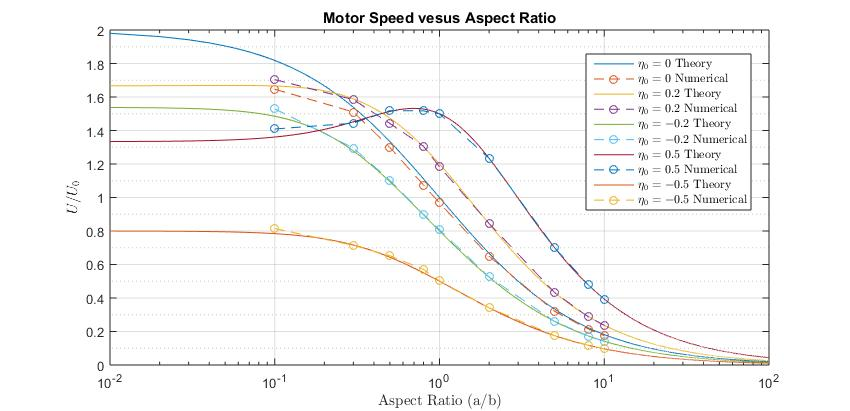
\includegraphics[width=\linewidth, height=3in]{2016-10-26-verification.jpg}
\caption{Verification of Moter With Source-Inert Configuration}\label{VoMWSIC-10-26-2016}
\end{figure}
The next step is to compare the motor speed in free space and within channel confinement.

\labday{Sunday, 30 October 2016}
When I model the motor within channel, the calculation results (Fig. \ref{ALSTEFL-10-26-2016}) show that there is a line(around pos=0.3/0.75) which seperates the upper part of electrical field and lower part of electrical field. I don't know how to determine the postion of this line or whether it is important for motor speed. I think it more or less relates to the geometry of motor as I set the uniform charge density on the surface of motor.
\begin{figure}
\centering
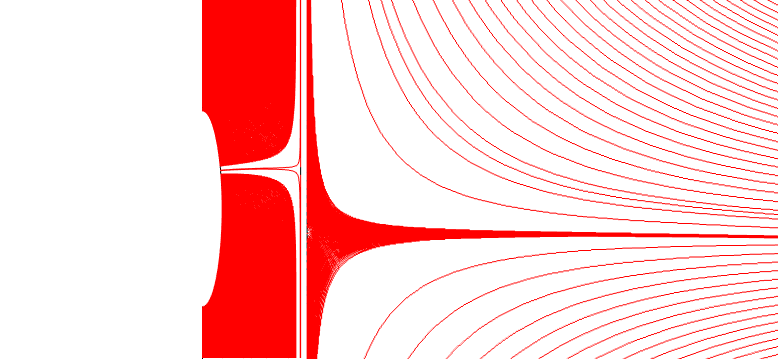
\includegraphics[width=\linewidth, height=3in]{2016-10-30-line.png}
\caption{A line seperates the electrical field lines}\label{ALSTEFL-10-26-2016}
\end{figure}

\labday{Monday, 31 October 2016}
\experiment{Paper000018}
This paper investigate the behavior of source/inert motor near plane wall. It considers both the translational motion and rotational motion of motor. Actually, the supplementary material of this paper is much useful for me. It presents the numerical method to solve this problem. Under infinitesimal thin EDL approximation, the gradient field could be decoupled from fluid field. Thus, we could solve the gradient field firstly (typically it's a Laplace equation). While, the boundary conditions of fluid field depends on the gradient field, we need substitute results into the fluid part. However, we care about the velocity of motor which should be determined by force and torque balance. Directly solving the motor velocity is not easy.\\
The author presents that we could utilize \emph{Lorentz Reciprocal Theorem} in Stokes flow to circumvent this difficulty. Construct some dual problems could be easily calculated and express our target problem by these dual problems' solution. In the case given by this paper, the solution of motor translational velocity and angular velocity could be expressed as the solution of a linear system. This provides me a good hint that how to calculate dynamics of motor in 3d space. It will be useful when I am ready to discuss force and torque balance of motor.
\\
Another thing need to mention is about numerical calculation. I calculated the case for source/inert motor within channel confinement. However, unlike the case for source/sink motor, source/inert motor doesn't show significant speed up within channel and it even decreases speed within channel. I still not very confident about this conclusion. These are some points need to clarify:
\begin{enumerate}
\item
The boundary condition for channel wall. I currently use electroosmostic boundary condition for channel wall. But I am not quiet sure the sign of mobility for wall.
\item
The numerical accuracy. I run computation several times with different mesh size. Sometimes auto-generated mesh will break down. Manual-generated mesh would be fine but the results seem sensitive to mesh size. I can't confirm the accuracy of my results. I need to find a analytic results for comparision.
\item
I also plot the electrical field (Fig. \ref{2016-10-31-EFL}) and velocity field (Fig. \ref{2016-10-31-VFL}) for source/inert motor. It shows totally different features compared with source/sink motor. These two figures are shown below: 
\begin{figure}
\centering
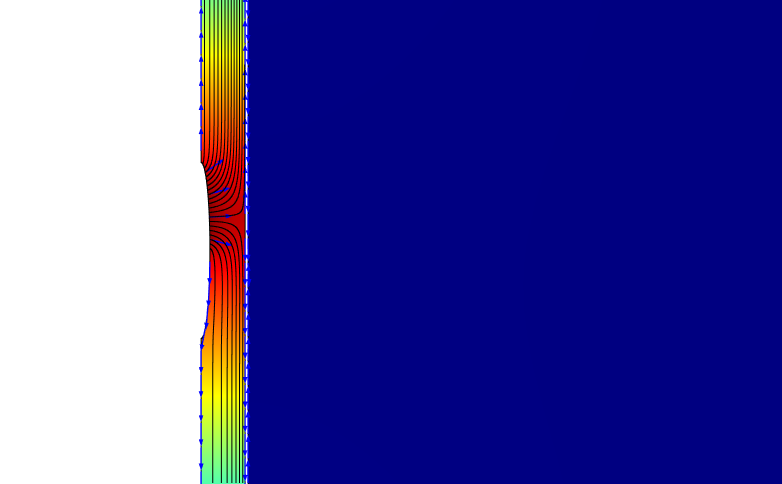
\includegraphics[width=\linewidth, height=3in]{2016-10-31-electrical-field.png}
\caption{Electrical Field Lines}\label{2016-10-31-EFL}
\end{figure}
\begin{figure}
\centering
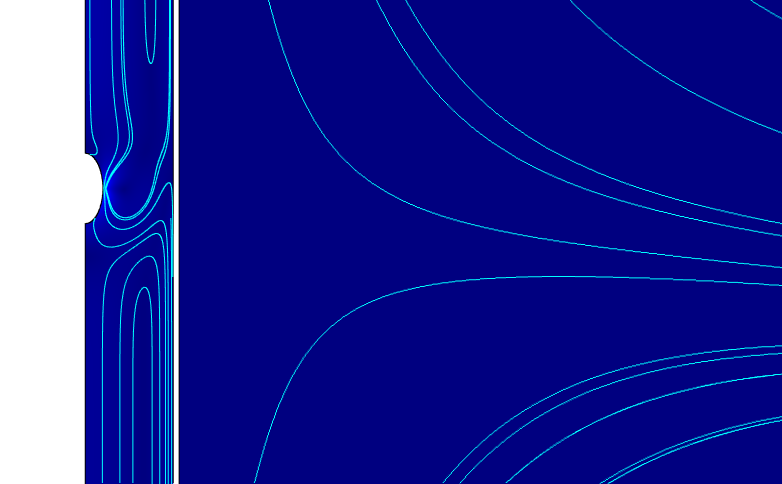
\includegraphics[width=\linewidth, height=3in]{2016-10-31-velocity-field.png}
\caption{Velocity Field Lines}\label{2016-10-31-VFL}
\end{figure}
\end{enumerate}

\labday{Tuesday, 1 November 2016}
Prepare Thesis Proposal. Basic Information is recorded below:
\begin{itemize}
\item Title: Artificial Microswimmer under spatial confinement
\item Supervisor: Prof. Zhang, Hepeng \& Prof. Xing, Xiangjun
\end{itemize}

\labday{Wednesday, 2 November 2016}
\experiment{Fourth Associated Group Meeting of Soft Matter, 2016 Autumn}
Title: First Passage Time Problems\\
Speaker: Yang, Xiang\\
This is the second time to hear this talk. I first hear this talk in Prof. Zhang's group meeting. The first passage time concerns the time of an random event first happening and is a very interesting problem which is worth endeavouring. First passage time is a very important concept in various fields, for example we may how long is needed for a particle move from position A to position b within a cell, how long will a neurotransmitter started from position A to the surface of  synapses then stimulate the signal or how long the price of one stock will fall in the stock market, etc. In my opinion, the concept of mean first passage time have a wide range of application in both nature and socioty. \\
The concept of mean first passage time(MFPT) is illustrated by the diffusion in 1D infinite system. The activation of an event is substituted by the absorbing boundary. The core equality which defined the distribution of MFPT is: the time derivative of survival probability(the integration of current probability density in whole space) is equal to the flux at absorbing boundary. Using image method could easily give the solution of 1D infinite system. Then, Yang Xiang discussed the case in higher dimension of infinite and finite system. Pay special attention to the fractal system where characteristic time scale could be related to the fractal dimension and walk dimension.

\labday{Thursday, 3 November 2016}
Two recent numerical results.
\begin{enumerate}
\item
The comparsion between motor speed in free space and in channel confinement.\\
As shown in Fig. \ref{2016-11-3-MSC}, the motor under channel confinement shows little speed up even speed down. The numerical errors make the point of aspect ratio 0.1 is excluded. However, consider the case of source/sink which shows speed up to five times, this result shows source/inert motor differs with source/sink significantly if the result is trustworthy. I want to inspect my modeling careful and theories I based on because I am still not sure about this calculation.
\begin{figure}
\centering
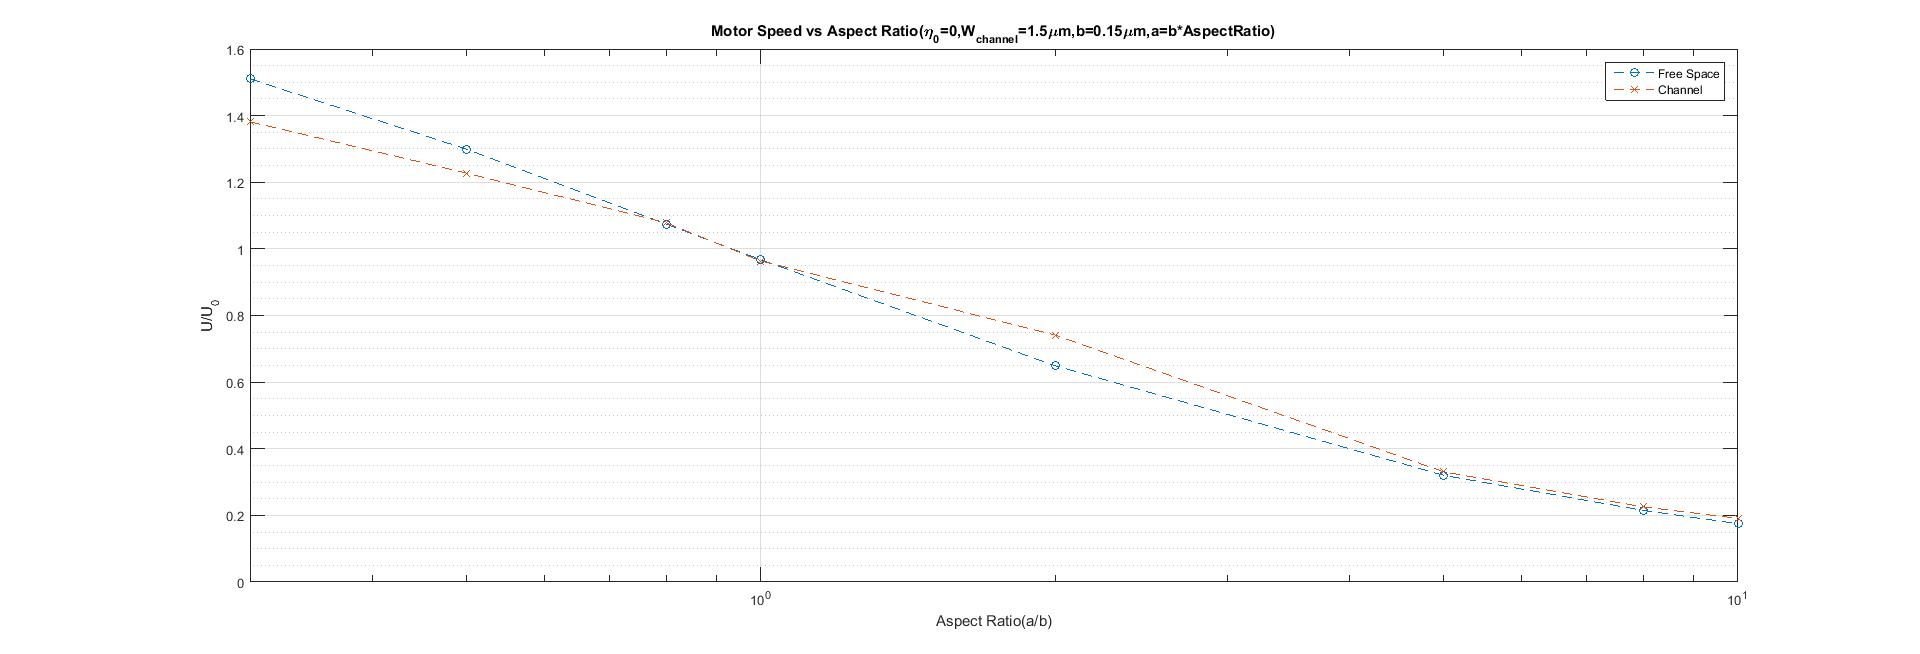
\includegraphics[width=\linewidth, height=3in]{2016-11-3-Channel.jpg}
\caption{Motor Speed Comparison}\label{2016-11-3-MSC}
\end{figure}
\item The motor speed with different degree of confinement.\\
As shown in Fig. \ref{2016-11-3-MSUCWDW}, the motor speed doesn't change significantly until channel width reaches around $1\mu m$. In the extreme confinement case ($0.5\mu m$), motor speed does inscrease significantly. However, in such a small confinement, my model may not be valid and I am suspicious about this result. It shows channel confinement speeds motor up which contradicts with previous case. I am wondering whether significant speed up will only occur in very small channel. I will check this suspect soon.
\begin{figure}
\centering
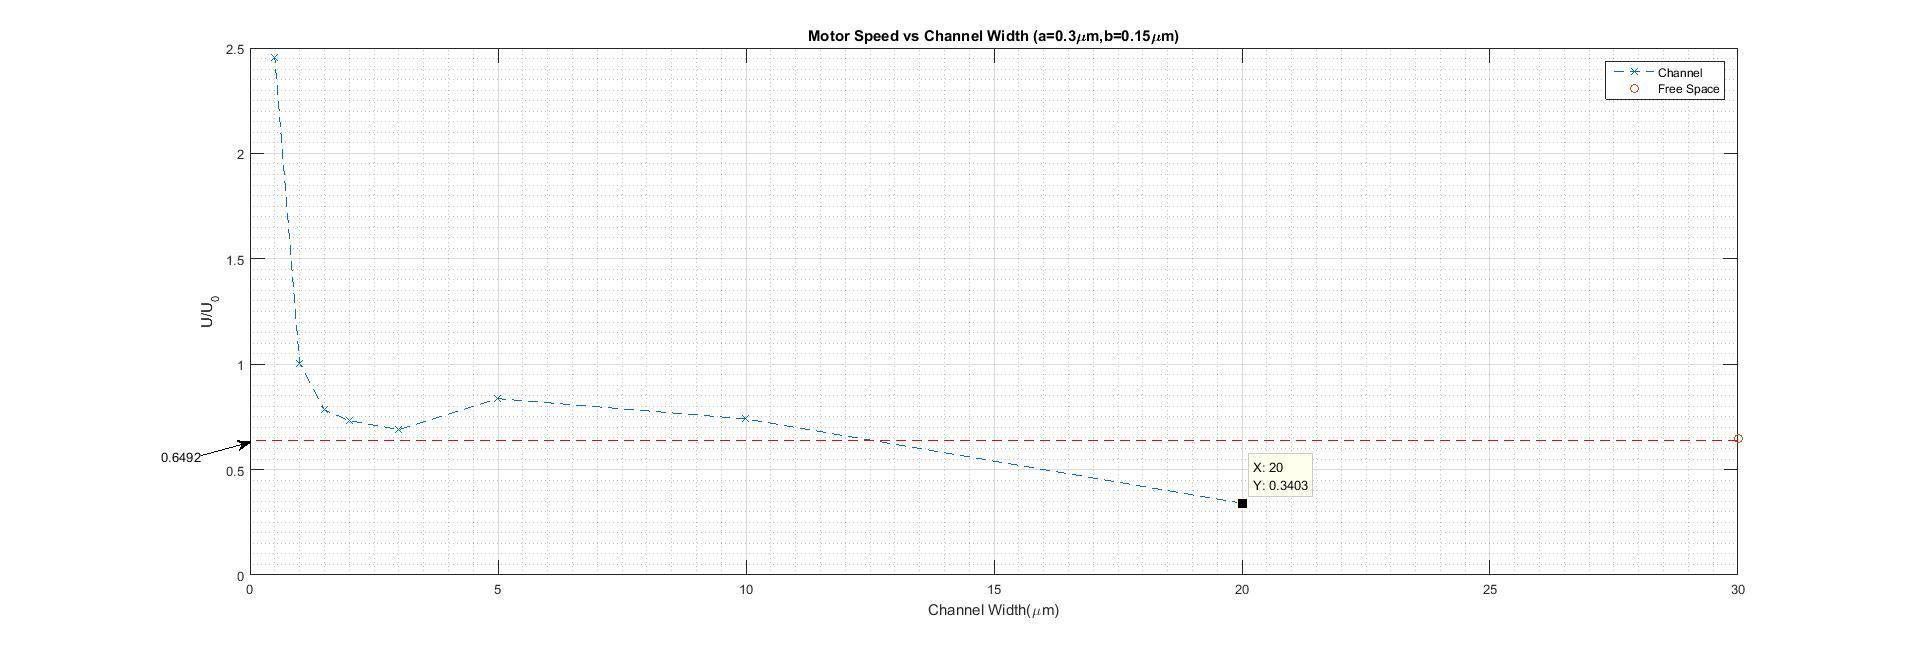
\includegraphics[width=\linewidth, height=3in]{2016-11-3-diff-channel-width.jpg}
\caption{Motor Speed Under Channel with Different Width}\label{2016-11-3-MSUCWDW}
\end{figure}
\end{enumerate}

\labday{Friday, 4 November 2016}
\experiment{Paper000019}
This paper concerns about the efficiency of microswimmers. The estimated efficiency of typical bimetallic rod-shape microswimmer is the order of $10^{-9}$ which is very inefficient compared with bio-motor, like kinesin-based microtubule motors. Four kinds of energy loss are discussed to explain the low efficiency of self-electrophoresis motos:
\begin{enumerate}
\item
Fuel loss through chemical decomposition: A large amount of chemical reactions are not electrochemical.
\item
Inefficient electrochemical cell: The chemical reaction will only generate limited potential drop upon the motor surface. I don't understand this point well.
\item
Inefficient particle transport mechanism: The gradient of proton can't maintain in a relative long time scale because of the large diffusion constant of proton. A possible method to keep the concentration gradient to establish large self-generated electrical field is to use spatial confinement, like tube-shape motor.
\item
Opposite electroosmostic flow: The boundary effect caused by wall. The wall is usually negatively charged in hydrogen peroxide and will interaction with charged motor surface. When the distance between motor and wall decreased to the order of Debye length, the self-generated electrical field will cause flow in cation-rich diffusion layer which is opposite to the direction of motor movement.
\end{enumerate}

\labday{Saturday, 5 November 2016}
Two new results:
\begin{enumerate}
\item
Moter Speed Under Different Degrees of Spatial Confinement\\
I check this relation with small steps of channel width (Fig. \ref{2016-11-5-MSUDCW}). Two points with large channel width are suspicious. The reason I still do not quite understand. The speed up of motor under spatial confinement occurs around 1$\mu m$ channel width. Some questions:
\begin{enumerate}
\item
The Localized Electroosmostic Flow will drag the motion of motor thus decrease the speed of motor?
\item
The debye length of wall ?
\item
The mechanism of speed up under spatial confinement? I need to clarify this further.
\end{enumerate}

\item
Motor Speed Under 1$\mu m$ Channel Wall With Different Aspect Ratio\\
I check the motor speed under more tight spatial confinement(Decrease channel width from $1.5 \mu m$ to $1 \mu m$, results are shown in Fig. \ref{2016-11-5-MSU1CW}). This time, the motor do show speed up in large aspect ratio which contradicts with previous result in $1.5\mu m$. This region is that the distance between motor and wall is relatively small (comparable to debye length?). \\
This is strange. Whether speed up will only occur in very tight spatial confinement. I need to check this further. 
\end{enumerate}
\begin{figure}
\centering
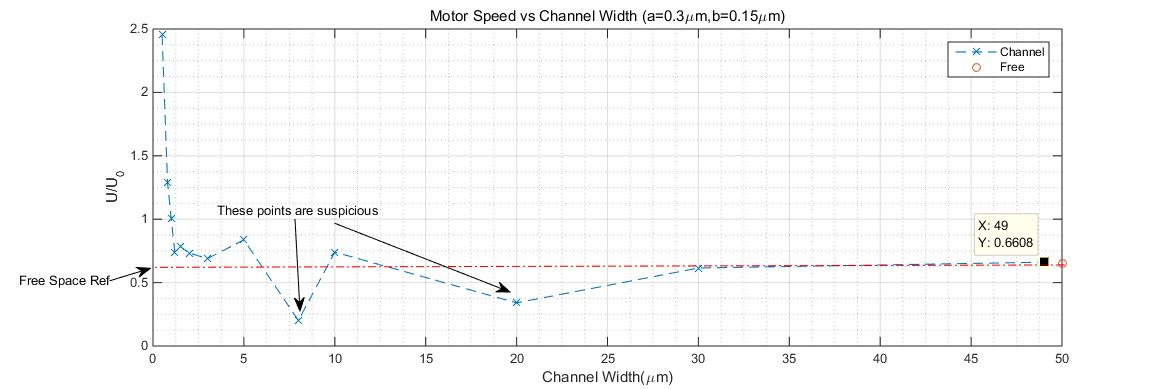
\includegraphics[width=\linewidth, height=3in]{2016-11-5-diff-channel-width.jpg}
\caption{Motor Speed Under Different Channel Width}\label{2016-11-5-MSUDCW}
\end{figure}

\begin{figure}
\centering
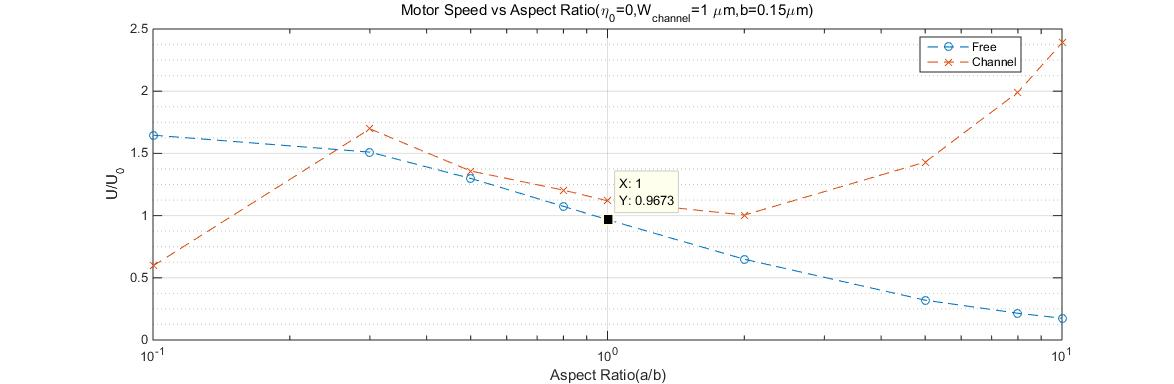
\includegraphics[width=\linewidth, height=3in]{2016-11-5-eta-0-wall-1.jpg}
\caption{Motor Speed Under 1$\mu m$ Channel Wall}\label{2016-11-5-MSU1CW}
\end{figure}

\labday{Sunday, 6 November 2016}
\experiment{Report 1 - Review from Sep. 19, 2016 to Nov. 5, 2016}
\section*{Introduction}
After approximate two months of work, it's time to summarize my current understanding of problem, discuss results and set up plan for next stage of research. The last two months, my main focus is to read relevant literatures about my thesis. I start from some "ancient" papers about motion of charged colloid under external electrical field to obtain some general theoritical framework. Also I read several papers about microswimmers to know some histories and general ideas in this field. Then, I mainly refer to papers of Velegol et al. and our group's paper to get some concepts and details related to the bimetallic motor I concern about. At the mean time, I also establish the numerical model for source/inert configuration motor in COMSOL with the reference to Liu Chang's model and do verification and some computations for source/inert motor in confined channel.\\
To sum up, I don't cover many literatures in this field before the thesis proposal as expected. While the numerical modeling costs less time than I expected because of Liu Chang's previous work. Now I begin to have some basic understanding of my thesis ( although limited) and I am ready to my stage of research.
\section*{Description}
Based on phenomenon of source/sink motor speed up in confined channel discoveried by our group\cite{Liu2016}, consider the corresponding case for source/inert motor. The work roughly divides into two parts:
\begin{enumerate}
\item
Verify the numerical model for source/inert motor in free space by comparing results with analytic expression in the paper of Nourhani and Lammert\cite{Nourhani2016}.
\item
Consider the numerical model for source/inert motor in confined channel
\end{enumerate}
\section*{Method}
In this section, I will list some key assumptions in my current model.
\subsection*{Theory}
\subsubsection{Surface of motor}
This part is based on Gouy-Chapman-Stern model. As shown in Fig. \ref{2016-11-13-GCSMFIIE}, the solution could be divided into three parts: Stern layer, Diffusion layer and Bulk solution. Typically, 
\begin{itemize}
\item The Stern layer has length scale of order of \AA \ which is fixed with motor surface.
\item The diffusion layer has length scale of order of several hundreds of nanometers (Debye length) for the case in hydrogen peroxide, which is cation-rich for negatively charged motor surface. 
\item The region beyond Stern layer and diffusion layer is the bulk solution which could be regarded as neutral.
\end{itemize}
In the paper \emph{Catalytically driven colloidal patterning and transport}\cite{Kline2006}, authors employ Nernst-Plank equation:
\begin{equation}
\v J_i=-D_i \nabla n_i + z_ien_i\v E_i \mu_i + \v v n_i
\end{equation}
and Poisson equation for electrostatic part:
\begin{equation}
\nabla^2\psi=-\frac{\sum_i z_i e n_i}{\epsilon}
\end{equation}
to solve the electrical field and particle concentration distribution within diffusion layer. \\
\emph{Ignore the convection term in flux and regard the chemical reaction on the motor surface as small perturbation}, the first-order perturbation could give the solution of above equations within diffusion layer which connnects surface activities ($\v J_i$) with electrical field $\v E$ at the outer edge of diffusion layer:
\begin{equation}
\v E = \frac{\v J k T}{2e D n_0}
\end{equation}
\subsubsection{Motor Speed in free space}
Antoher work in paper \emph{Geometrical Performance of Self-Phoretic Colloids and Microswimmers}\cite{Nourhani2016} express the motor speed in surface integration of surface activities:
\begin{equation}
U=\uv{e}_z \frac{-\mu_{ph}}{2D}\int_{-1}^1 K(\eta;a/b)\Gamma(\eta)\mathrm{d}\eta
\end{equation}
where
\begin{equation}
K(\eta;a/b)=\frac{\eta}{\sqrt{\eta^2+(a/b)^2(1-\eta^2)}}
\end{equation}
and
\begin{equation}
\Gamma=-D\uv n \cdot \nabla \gamma
\end{equation}
$\gamma$ is a possible field(like electrical field, concentration field) and $D$ is the constant corresponding to it (like diffusion constant).\\
Thus, I apply this result to my model with previous approximation. \emph{Regard $\gamma$ as electrical potential $\phi$, then $\Gamma$ is the electrical field $\v E$ at the outer edge of diffusion layer.} It means that I actually set the boundary of model at the outer edge of diffusion layer but not the surface of motor. However, as long as the approximation of infinitesimal electrical double layer is valid, I still accept this approximation is reasonable.\\
With this simplifiction, \emph{all the calculation domain should be neutural}. Thus, there is no need to consider the transportation of ions.
\subsubsection{Electroosmosis Flow}
However, the electroosmosis flow must be taken into consideration for correct calculation in confined space \cite{ChiangVelegol2014}. If the solution is neutral, electroosmosis cannot happen. This electroosmosis only happens within the diffusion layer. Then, the moving of ions within diffusion layer will result in the flow in bulk solution which is the electroosmosis flow I refer to in the section title. \\
Because I apply the thin EDL approximation, there is no diffusion layer in calculation domain. The effect caused by electroosmosis flow must reflect by appropriate boundary conditions. Therefore, both boundary conditions in channel wall and motor surface should be electroosmosis boundary condition which requires that fluid velocity should be propotional to tangential electrical field:
\begin{equation}
\v v_{eo}=\mu \v E_t
\end{equation}
where $\mu$ is the corresponding mobility and is propotional to zeta potential.
\begin{figure}
\centering
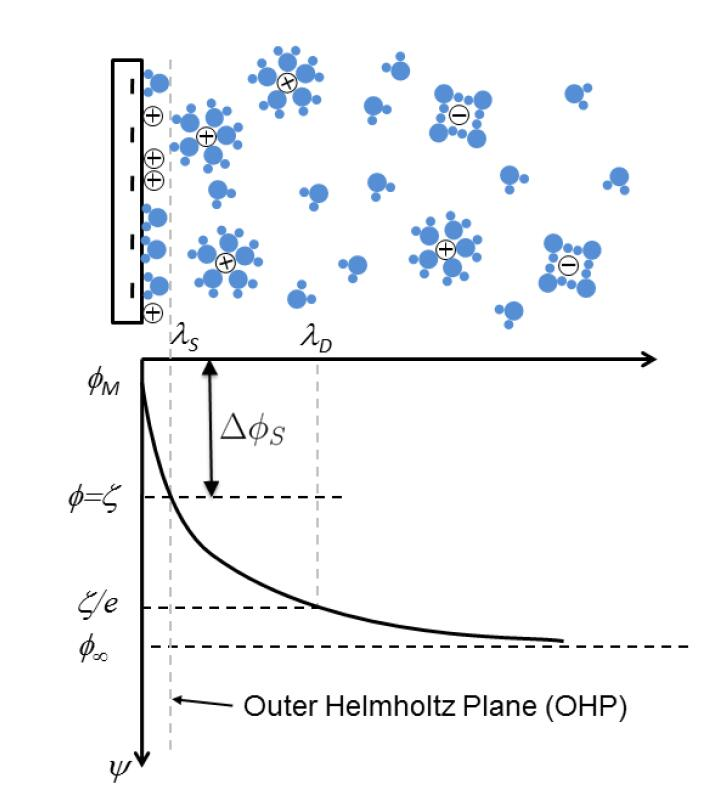
\includegraphics[width=\linewidth, height=6in]{2016-11-13-Interface.jpg}
\caption{Gouy-Chapman-Stern model for Interface in Electrolyte}\label{2016-11-13-GCSMFIIE}
\end{figure}

\subsection*{Computation}
With above consideration, the details of my numerical model in COMSOL are following:
\subsubsection{Electrostatic Part}
\begin{itemize}
\item Governing equation (no charge in bulk) :
\begin{equation}
\nabla^2\psi=0
\end{equation}
\item Boundary conditions:
\begin{enumerate}
\item
Constant charge density condition for active surface of motor
\begin{equation}
\sigma=constant
\end{equation}
\item
Zero charge density condition for inert surface of motor
\begin{equation}
\sigma=0
\end{equation}
\item
Zero charge condition for channel wall and bulk solution
\begin{equation}
\rho=0
\end{equation}
\item
Zero potential condition for outer edge of simulation domain
\begin{equation}
\psi=0
\end{equation}
\end{enumerate}
\end{itemize}
\subsubsection{Fluid Part}
\begin{itemize}
\item Governing equation:
\begin{equation}
\eta \nabla^2 \v u = \nabla P
\end{equation}
\begin{equation}
\nabla \cdot \v u =0
\end{equation}
\item Boundary conditions:
\begin{enumerate}
\item
Electroosmosis condition for channel wall:
\begin{equation}
\v u = \mu_{wall} \v E_t
\end{equation}
\item
Electroosmosis+motor speed for motor surface:
\begin{equation}
\v u = \mu_{motor} \v E_t + v_{motor}
\end{equation}
\item
No slipping condition for outer edge of simulation domain:
\begin{equation}
\v u =0
\end{equation}
\end{enumerate}
\end{itemize}
\section*{Result}
I did several calculations with above defined problem. Results are summerized below:
\subsection*{Verification}
The first is the verification of my numerical model. I do a comparision for source/inert motor in free space as shown in Fig. \ref{2016-11-13-CBNRAAR}. It shows good agreement as long as the aspect ratio is not too small. (For small aspect ratio, the mesh cannot work well). This results support above assumptions I made in my model.
\begin{figure}
\centering
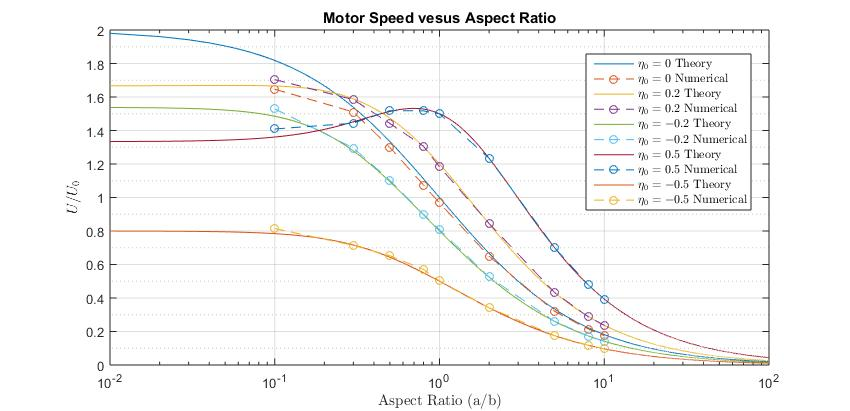
\includegraphics[width=\linewidth, height=3in]{2016-10-26-verification.jpg}
\caption{Comparision Between Numerical Results and Analytic Results}\label{2016-11-13-CBNRAAR}
\end{figure}
\subsection*{Add Channel For Source/Inert Motor}
With above confirmation, I add a channel wall into my model and compare it with results in free space as shown in Fig. \ref{2016-11-13-CBFACC}. Unlike source/sink motor shows significant speed up, source/inert motor does not show significant speed up. Note that here I choose channel width as $1.5 \mu m$.
\begin{figure}
\centering
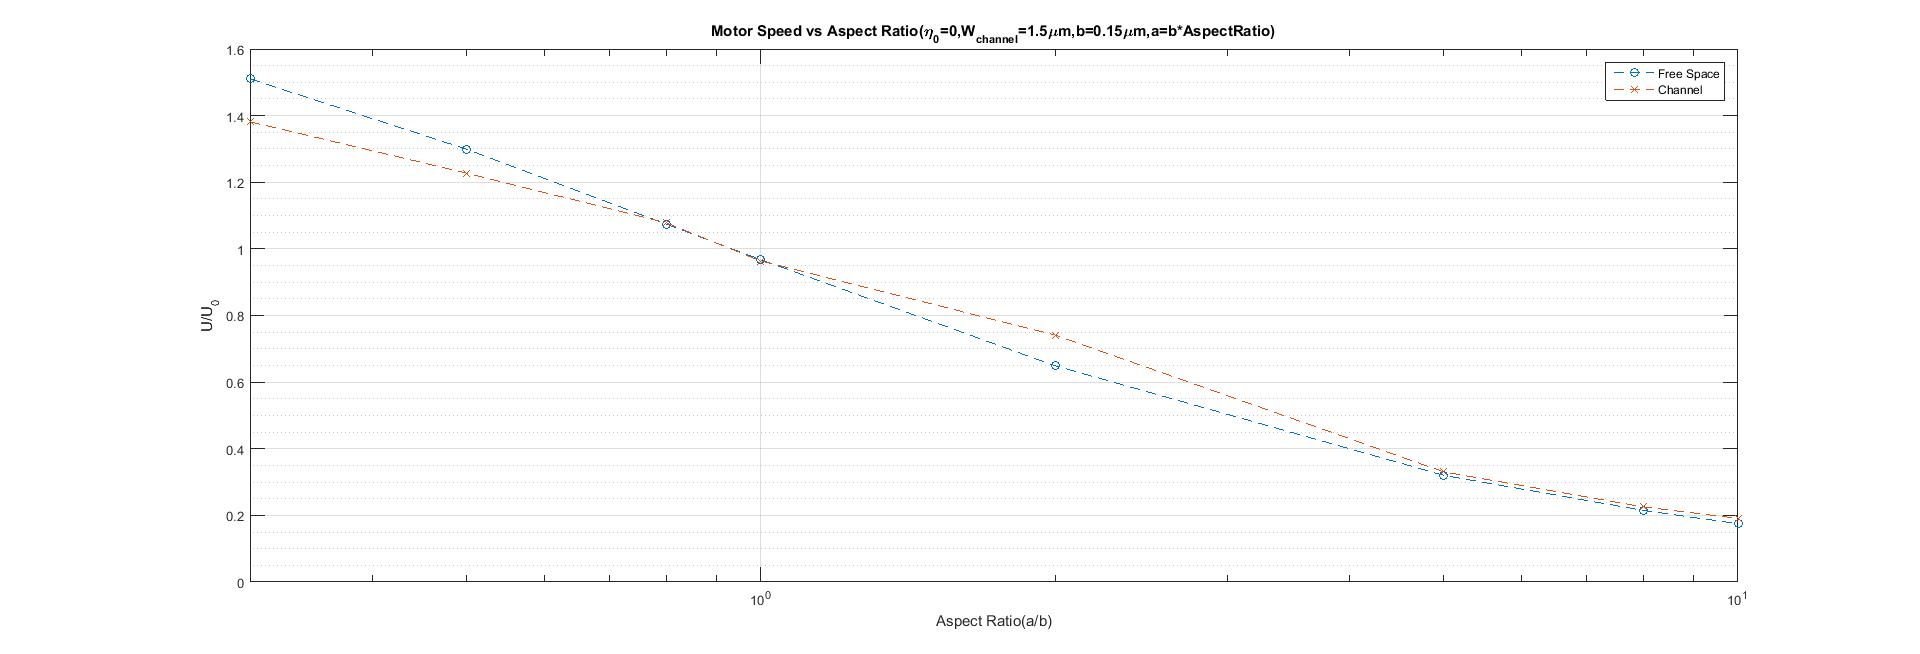
\includegraphics[width=\linewidth, height=3.5in]{2016-11-13-eta-0.jpg}
\caption{Comparision Between Free and Confined Case}\label{2016-11-13-CBFACC}
\end{figure}
\subsection*{Speed Change Under Different Channel Width}
In order to check speed change of source/inert motor under channel confinement, I plot the motor speed vesus different channel width as shown in Fig. \ref{2016-11-13-SCUDCW}. This result makes me confused. The motor does show speed up for very narrow channel (less than 1 $\mu m$) while does not show significant speed up for relatively wide channel (large than 1 $\mu m$). \\
Another point is that I think I have chosen very fine mesh for calculation. However, I can't obtain a smooth curve like the one for source/sink motor\cite{Liu2016}. I will confirm this further.
\begin{figure}
\centering
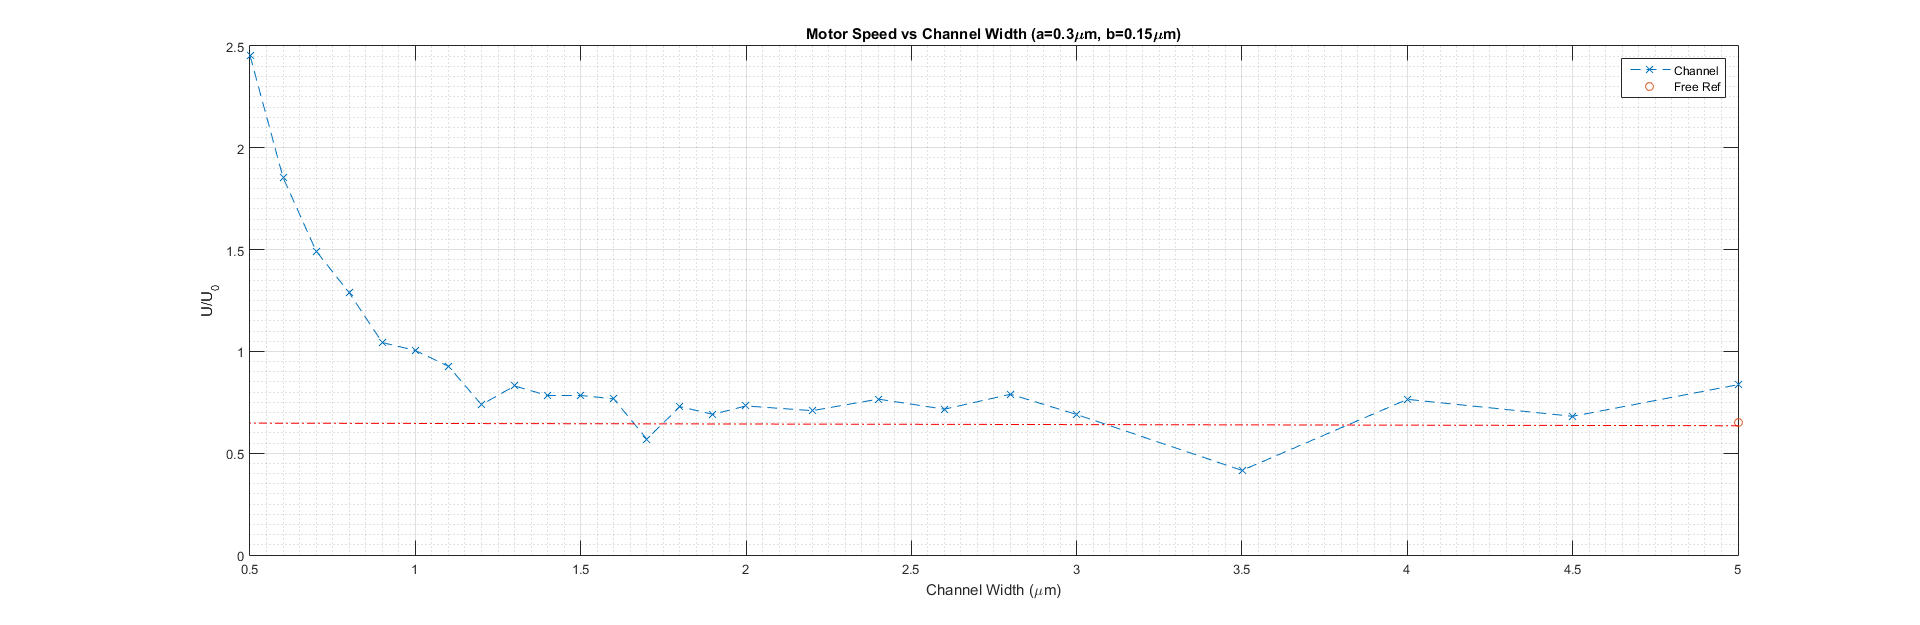
\includegraphics[width=\linewidth, height=3.5in]{2016-11-13-DiffCWidth.png}
\caption{Speed Change Under Different Channel Width}\label{2016-11-13-SCUDCW}
\end{figure}
\subsection*{Comparison between Source/Sink and Source/Inert}
In order to understand the different behavior between source/inert and source/sink motor, I compare their localized electrical field and fluid field.
\subsubsection*{Electrical Field and Fluid Field $(\zeta_{motor}=-50mV \zeta_{wall}=-50 mV)$}
\begin{itemize}
\item Source/Sink Motor (Fig. \ref{2016-11-13-EFOSSM} and Fig. \ref{2016-11-13-FFOSSM}):
\begin{figure}
\centering
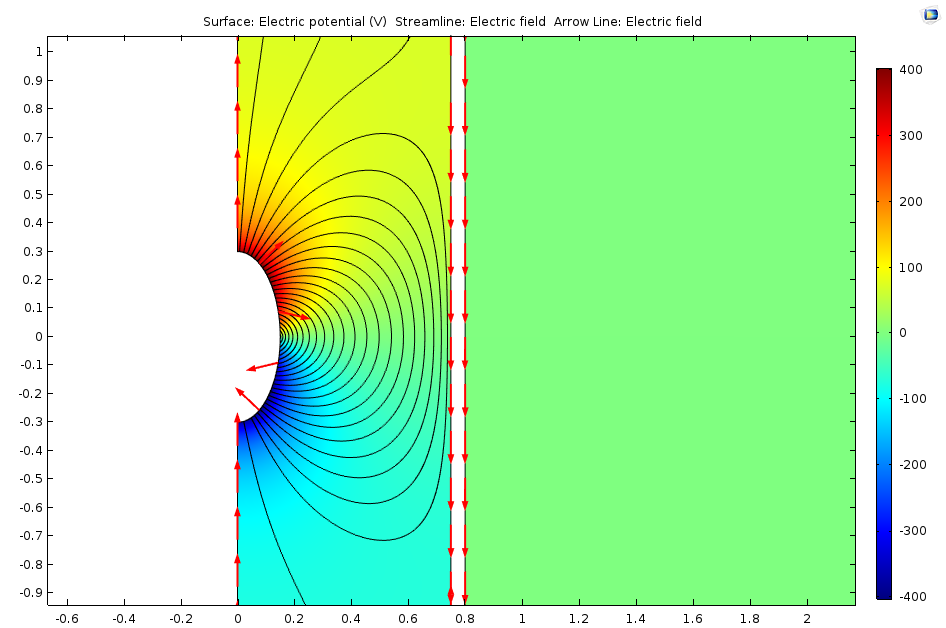
\includegraphics[width=\linewidth, height=3.5in]{2016-11-13-SourceSink-E.png}
\caption{Electrical Field of Source/Sink Motor}\label{2016-11-13-EFOSSM}
\end{figure}
\begin{figure}
\centering
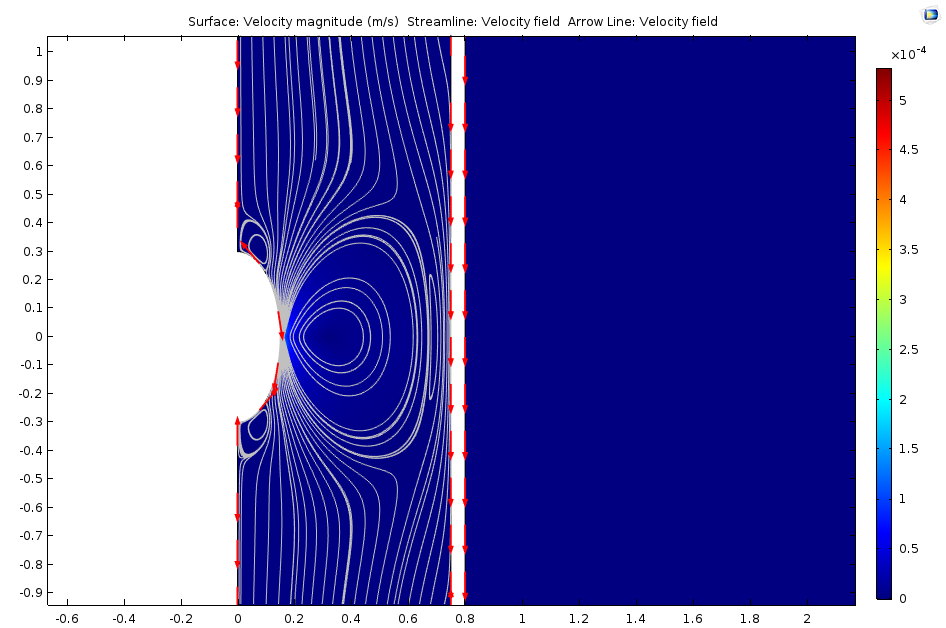
\includegraphics[width=\linewidth, height=3.5in]{2016-11-13-SourceSink-V.png}
\caption{Fluid Field of Source/Sink Motor}\label{2016-11-13-FFOSSM}
\end{figure}
\item Source/Inert Motor(Fig. \ref{2016-11-13-EFOSIM} and Fig. \ref{2016-11-13-FFOSIM}):
\begin{figure}
\centering
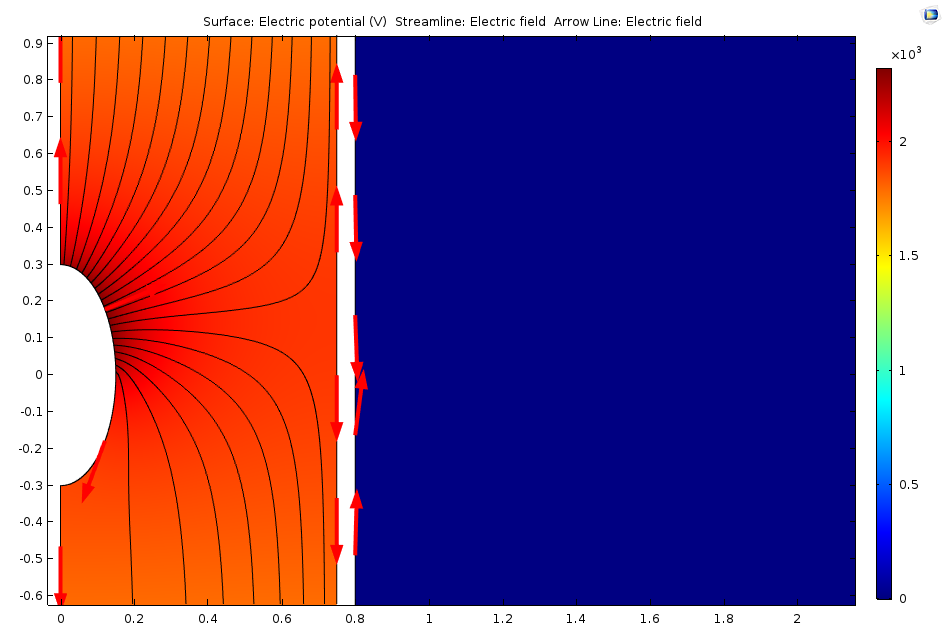
\includegraphics[width=\linewidth, height=3.5in]{2016-11-13-SourceInert-E.png}
\caption{Electrical Field of Source/Inert Motor}\label{2016-11-13-EFOSIM}
\end{figure}
\begin{figure}
\centering
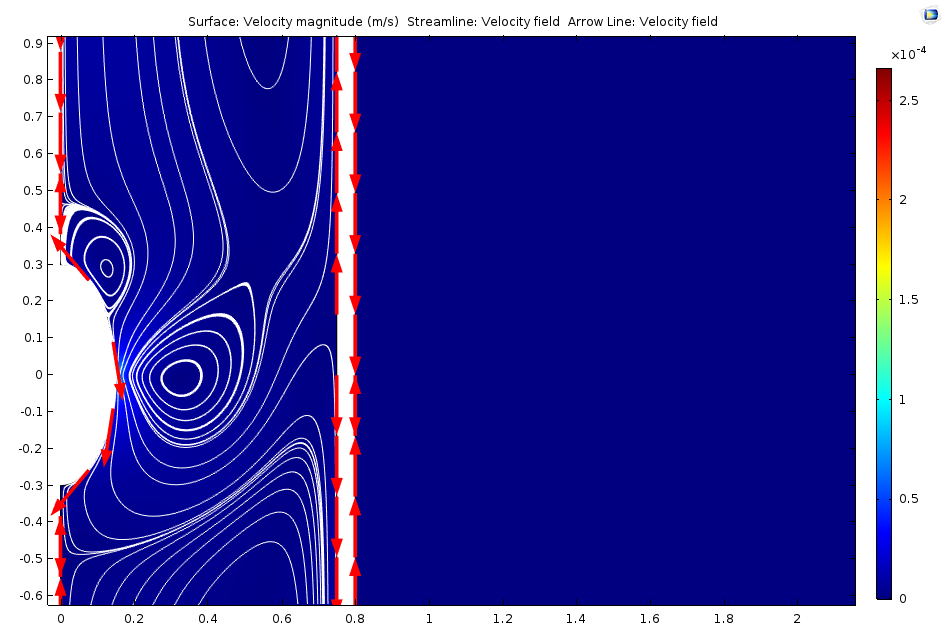
\includegraphics[width=\linewidth, height=3.5in]{2016-11-13-SourceInert-V.png}
\caption{Fluid Field of Source/Inert Motor}\label{2016-11-13-FFOSIM}
\end{figure}
\end{itemize}
\subsubsection*{Electrical Field and Fluid Field $(\zeta_{motor}=-50mV \zeta_{wall}= 0 mV)$}
\begin{itemize}
\item Source/Sink Motor $(\zeta_{motor}=0)$ (Fig. \ref{2016-11-13-EFOSSMM0} and Fig. \ref{2016-11-13-FFOSSMM0})
\begin{figure}
\centering
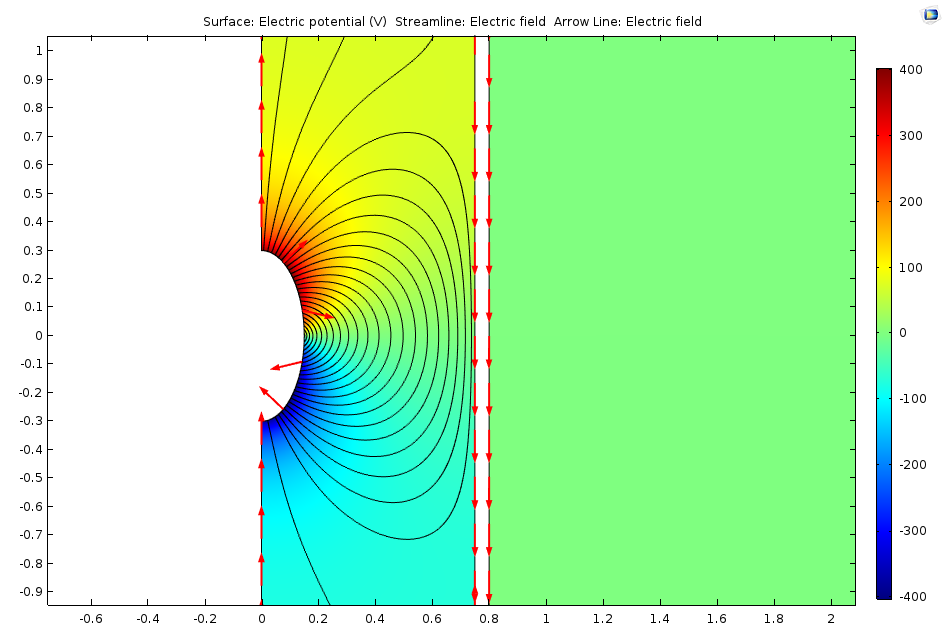
\includegraphics[width=\linewidth, height=3.5in]{2016-11-13-SourceSink-E-Osmosis.png}
\caption{Electrical Field of Source/Sink Motor $(\zeta_{motor}=0)$}\label{2016-11-13-EFOSSMM0}
\end{figure}
\begin{figure}
\centering
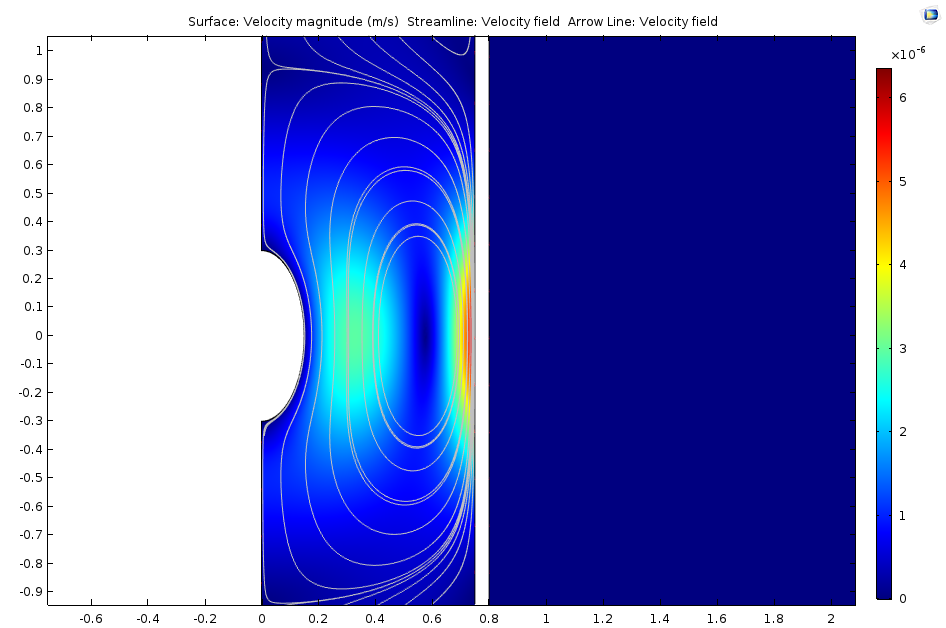
\includegraphics[width=\linewidth, height=3.5in]{2016-11-13-SourceSink-V-Osmosis.png}
\caption{Fluid Field of Source/Sink Motor $(\zeta_{motor}=0)$}\label{2016-11-13-FFOSSMM0}
\end{figure}
\item Source/Inert Motor $(\zeta_{motor}=0)$ (Fig. \ref{2016-11-13-EFOSIMM0} and Fig. \ref{2016-11-13-FFOSIMM0})
\begin{figure}
\centering
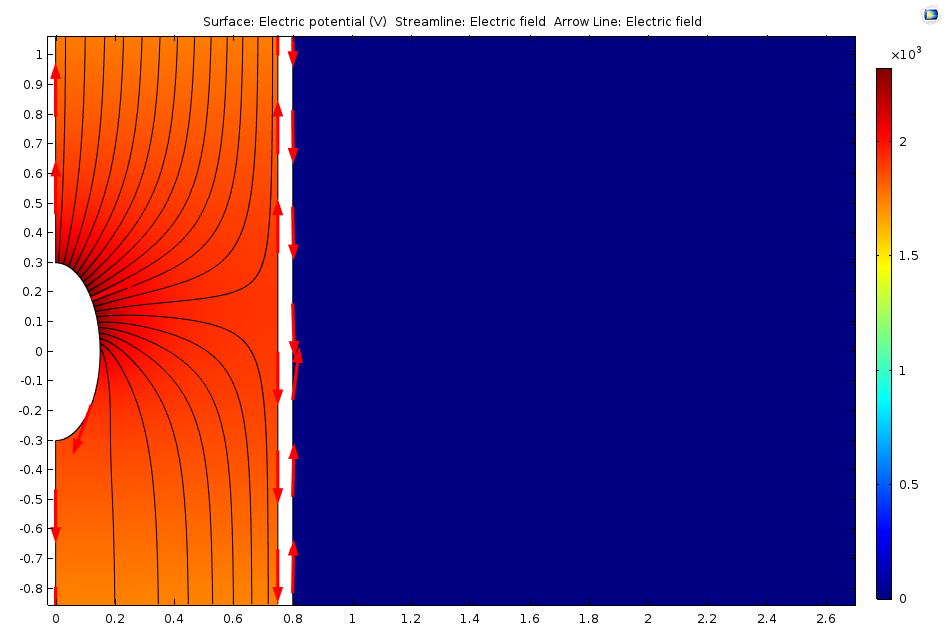
\includegraphics[width=\linewidth, height=3.5in]{2016-11-13-SourceInert-E-Osmosis.png}
\caption{Electrical Field of Source/Inert Motor $(\zeta_{motor}=0)$}\label{2016-11-13-EFOSIMM0}
\end{figure}
\begin{figure}
\centering
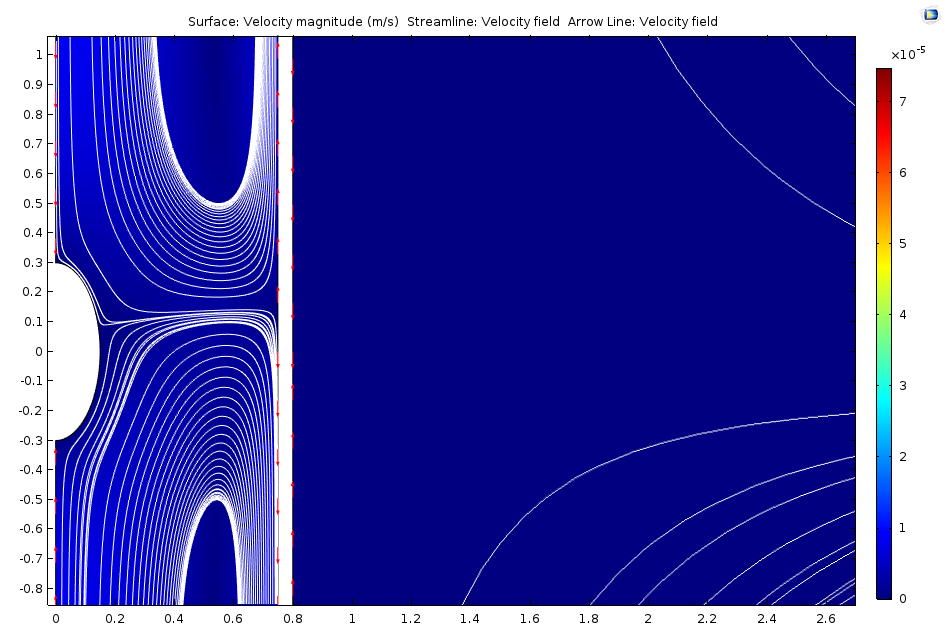
\includegraphics[width=\linewidth, height=3.5in]{2016-11-13-SourceInert-V-Osmosis.png}
\caption{Fluid Field of Source/Inert Motor $(\zeta_{motor}=0)$}\label{2016-11-13-FFOSIMM0}
\end{figure}
\end{itemize}
\subsubsection*{Electrical Field and Fluid Field $(\zeta_{motor}=0 mV \zeta_{wall}=-50 mV)$}
\begin{itemize}
\item Source/Sink Motor $(\zeta_{wall}=0)$ (Fig. \ref{2016-11-13-EFOSSMW0} and Fig. \ref{2016-11-13-FFOSSMW0})
\begin{figure}
\centering
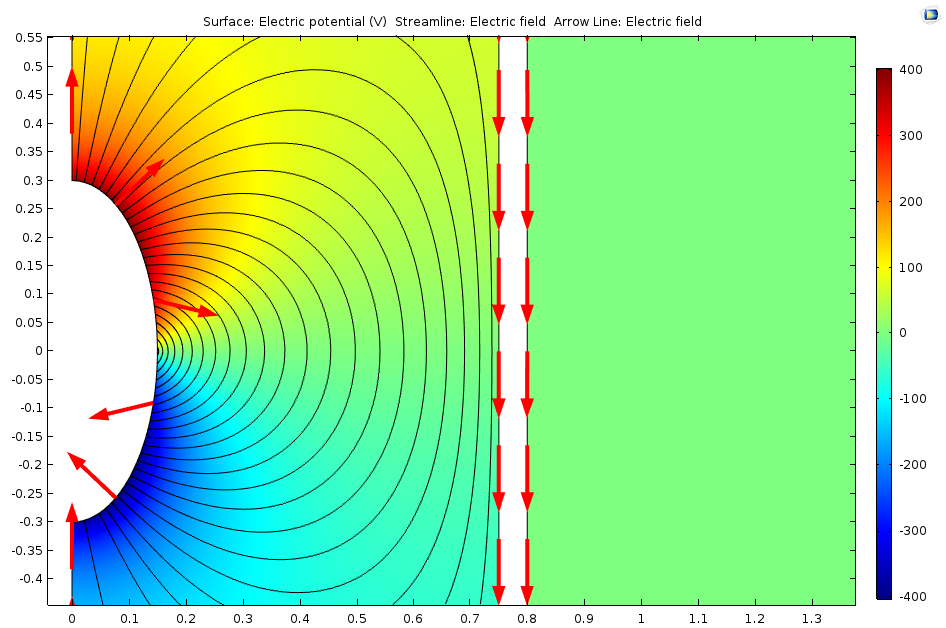
\includegraphics[width=\linewidth, height=3.5in]{2016-11-13-SourceSink-E-Motor.png}
\caption{Electrical Field of Source/Sink Motor $(\zeta_{wall}=0)$}\label{2016-11-13-EFOSSMW0}
\end{figure}
\begin{figure}
\centering
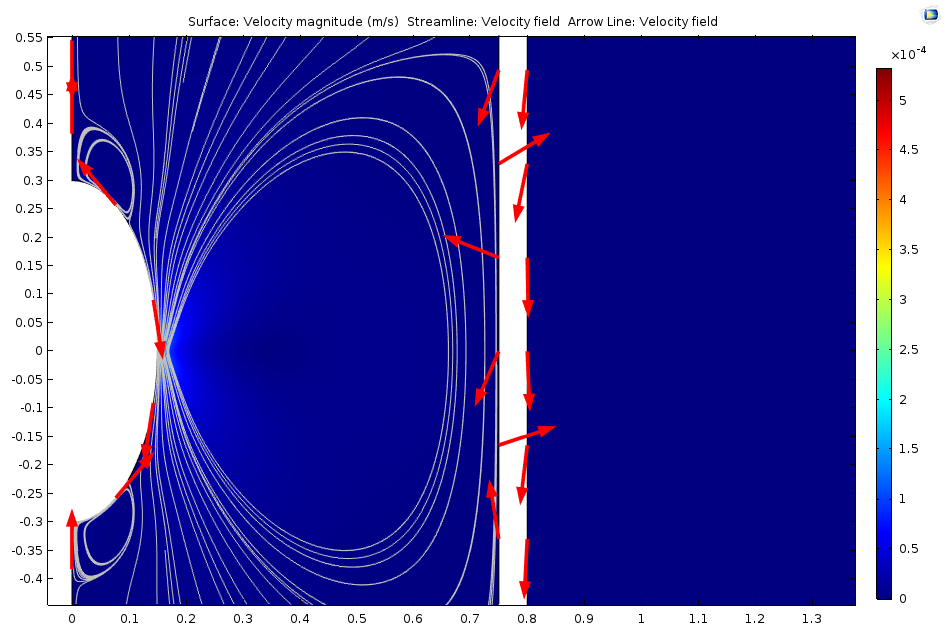
\includegraphics[width=\linewidth, height=3.5in]{2016-11-13-SourceSink-V-Motor.png}
\caption{Fluid Field of Source/Sink Motor $(\zeta_{wall}=0)$}\label{2016-11-13-FFOSSMW0}
\end{figure}
\item Source/Inert Motor $(\zeta_{wall}=0)$ (Fig. \ref{2016-11-13-EFOSIMW0} and Fig. \ref{2016-11-13-FFOSIMW0})
\begin{figure}
\centering
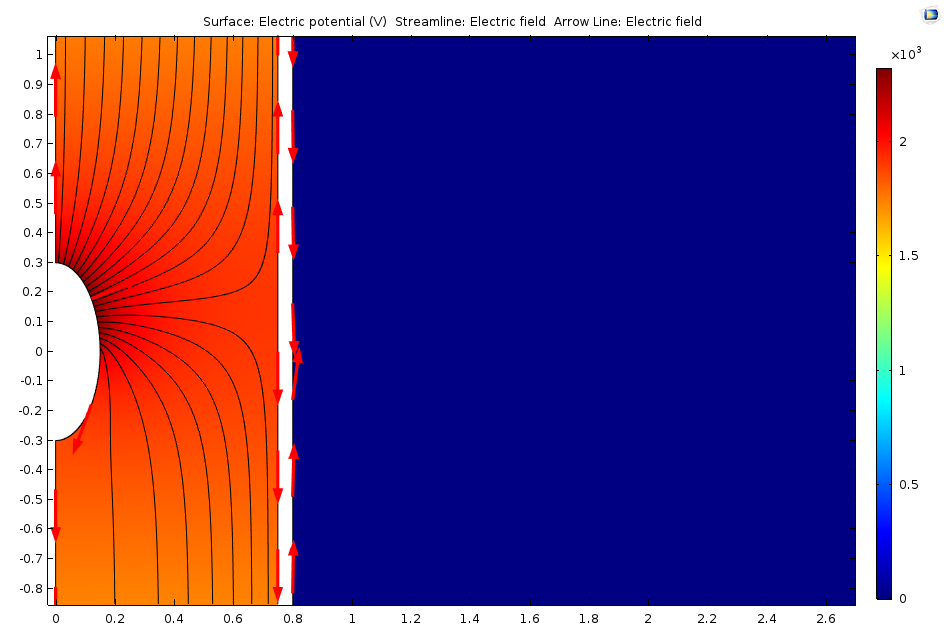
\includegraphics[width=\linewidth, height=3.5in]{2016-11-13-SourceInert-E-Motor.png}
\caption{Electrical Field of Source/Inert Motor $(\zeta_{wall}=0)$}\label{2016-11-13-EFOSIMW0}
\end{figure}
\begin{figure}
\centering
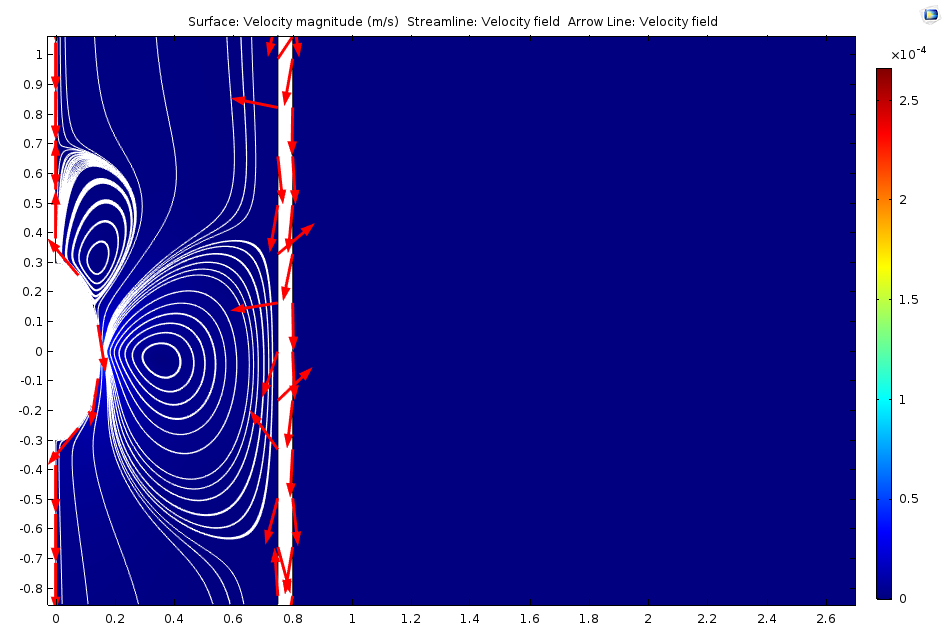
\includegraphics[width=\linewidth, height=3.5in]{2016-11-13-SourceInert-V-Motor.png}
\caption{Fluid Field of Source/Inert Motor $(\zeta_{wall}=0)$}\label{2016-11-13-FFOSIMW0}
\end{figure}
\end{itemize}

\labday{Friday, 11 November 2016}
\experiment{Fifth Associated Group Meeting of Soft Matter, 2016 Autumn}
Title: Neutron Scattering, Protein Glass Transition and Bosonic Peak\\
Speaker: Hong, Liang\\
Reserved.

\labday{Monday, 14 November 2016}
Wrong! Wrong! Wrong!\\
Today is a sad day. I cannot recover the results for source/sink motor in paper\cite{Liu2016} with my model, which means that my previous calculation could be all wrong!!!!\\

When I see my results, the one consider the motor speed under various channel width, I also don't trust my numerical simulation results. This model is a highly simplified model and completely linear. I can't believe my such irregular trends. \\
\begin{enumerate}
\item
I check the Liu Chang's model, it recovers results perfectly.\\
\item
I check the possibility of errors caused by mesh. But the results still don't make sense when I change the mesh. However, a strange thing is that the simulation results depend on mesh. Only from this point, it means that my current results are totally untrustworthy! \\
\item
I check the possibility of errors caused by scale. Because my model dimension is only on the order of $\mu m$, I guess COMSOL cannot handle this small defect in a large simulation domain correctly or my solver configuration is not correct. No matter what, I change the dimension of my model to a larger scale to check this hypothesis. The result could be obtained tomorrow.
\item
If the problem still cannot be solved, what other factors could be possible reasons? Errors come from where? I don't know yet. However, one thing is for sure: all my previous results are not reliable... I have to check and analyse previous work again to make sure my previous conclusions are correct... That is a sad story. 
\end{enumerate}

\labday{Thursday, 17 November 2016}
The results support my hypothesis to some extend. The results of larger aspect ratio (here I set it to 6, the same as Liu Chang's model) show better agreement with results in paper\cite{Liu2016}. It strengthens my confidence that errors are caused by the spheroid boundary in my model while the boundary of in Liu's model is just straight line. I guess COMSOL is not good at handling curved boundary.\\
In order to check my guess. I will do two simulations today:
\begin{enumerate}
\item
Change the aspect ratio of Liu's model to small value, from 6 to 2; To check whether results would be still consistent with results with large aspect ratio
\item
Change the boundary of my model to rectilinear case. To check whether results would be consistent with Liu's results
\end{enumerate}
I swear I will find the problem!!!

\labday{Friday, 18 November 2016}
I have to admit that yesterday's two numerical experiments both failed. The first one is approximately consistent with previous resutls. It confirms Liu's model; The second one still exhibits few irrugularities which are not expected. I previously thought the reason is because I specified a discontinuous boundary condition. I almost convinced myself to this explanation. However, today's results don't support this. That would be terrible.\\
I have another possble explanation to check: the extra point on rectilinear boundary inserted in my model. I have no better guess now although I don't expect too much on this test.\\
!!!!!!!! Oh my god! How could this be? This most unlikely explanation solve my problem!!! How could an extra point affects results in such a significant way in COMSOL??? CAN'T BELIEVE IT. Finally, my results become reasonable. For safety, I plan to check this model further to avoid similar mistake! \\
Now, I can enjoy my nice weekend! \\
The decisive results are recorded below in Fig. \ref{2016-11-18-ROMWOEP} and Fig. \ref{2016-11-18-ROMWTP}. One point spoiled everything...
\begin{figure}
\centering
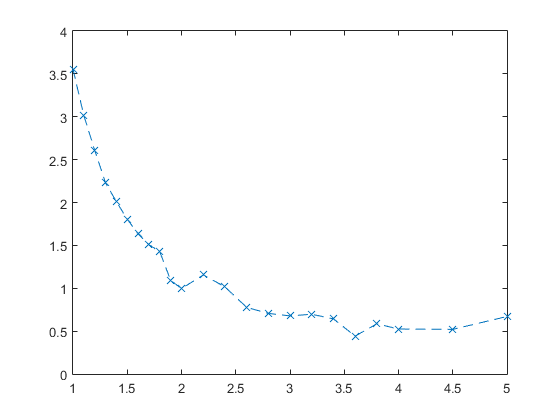
\includegraphics[width=\linewidth, height=3.5in]{2016-11-18-SourceSink.png}
\caption{Result of model with one extra point}\label{2016-11-18-ROMWOEP}
\end{figure}
\begin{figure}
\centering
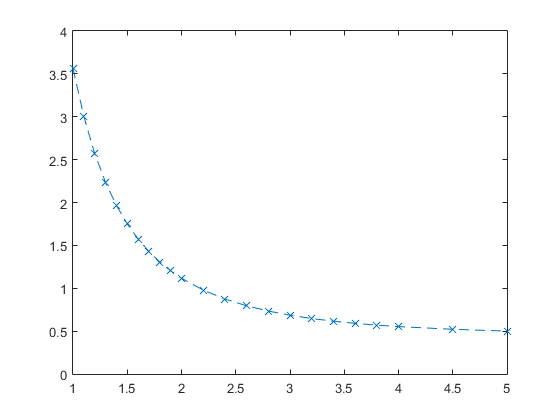
\includegraphics[width=\linewidth, height=3.5in]{2016-11-18-SourceSink-New.png}
\caption{Result of model without that point}\label{2016-11-18-ROMWTP}
\end{figure}

\labday{Sunday, 20 November 2016}
I rewrite my model and unify the cases for both source/inert configuration and source/sink configuration. Also, replace all discontinuous boundary conditions with continuous approximation. Introduce parameters for controlling various proportion of catalytic surface. I plan to recheck all my previous results with my fixed model in two days. Some experiments for today:
\begin{enumerate}
\item
Compute Source/Sink Rectangular Motor Speed Under Various Channel Confinement\\
Purpose: Compare with Liu Chang's Results\\
Calculation Finished. Data will be processed tomorrow.
\item
Compute Source/Sink Rectangular Motor Speed Under A fixed Channel Width with Different Mesh Accuracy.\\
Purpose: Check whether results converge with different mesh accuracy\\
Calculation Finished. Data will be processed tomorrow.
\item
Compute Source/Inert Spheroid Motor Speed With Different Aspect Ratio\\
Purpose: Compare with Analytic Result\\
Calculation In Progress.
\item
Compute Source/Inert Spheroid Motor Speed Under Various Channel Confinement\\
Purpose: Check Influence of channel confinement upon motor speed\\
Postpone to tomorrow.
\end{enumerate}

One major understanding of today's work is: boundary layer is crucial for the stability of numerical result. Numerical result must make sense in physics firstly.

\labday{Monday, 21 November 2016}
Data process of yesterday's calculation:
\begin{enumerate}
\item
Source/Sink Rectangular and Spheroid Motor Under Various Channel Confinement(Fig. \ref{2016-11-21-MSVDCW}):
\begin{figure}
\centering
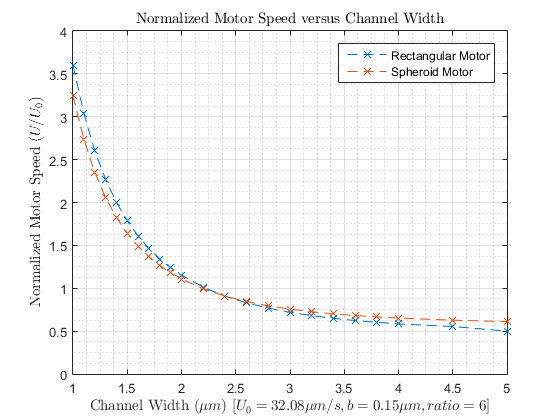
\includegraphics[width=\linewidth, height=4in]{2016-11-21-Speed-Diff-CWidth.png}
\caption{Motor Speed versus Different Channel Width}\label{2016-11-21-MSVDCW}
\end{figure}
\item
Mesh Independence Test. I want to make sure numerical result is independent of mesh choice. Results (Fig. \ref{2016-11-21-MT}) collapse into one curve.
\begin{figure}
\centering
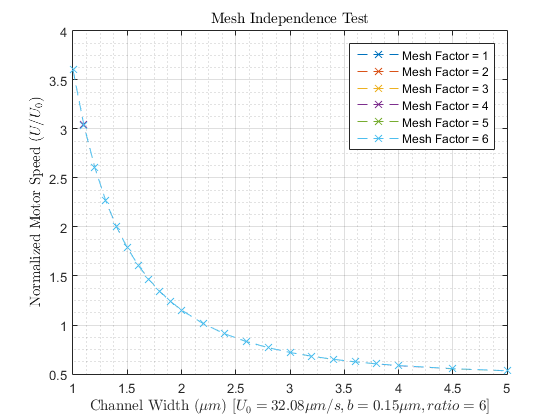
\includegraphics[width=\linewidth, height=4in]{2016-11-21-MeshTest.png}
\caption{Mesh Test}\label{2016-11-21-MT}
\end{figure}
\item A mistake found. Solved. Re-calculation in progress.
\item Calculation did not converge... postponed.
\end{enumerate}

\labday{Tuesday, 22 November 2016}
Analytic verification of spheroid motor with Source/Inert configuration in free space finished. The result is shown in Fig. \ref{2016-11-22-BWASIFS}. Numerical result agrees well with analytic result in the region where aspect ratio is larger than 1.5. For the region where aspect ratio is smaller than 1.5, the results seem unstable. Some calculation parameters are recorded here for later reference: $b=0.15 \mu m$, $a=ratio*b$, $MeshFactor=4$.\\
I still cannot accurately calculate the region where aspect ratio is smaller than 1.5. In that region, the geometry is too small and current mesh cannot work well. However, the result confirm the validity of my model in most common region where experiment would be carried on. Thus, I will move on and leave this problem unsolved.
\begin{figure}
\centering
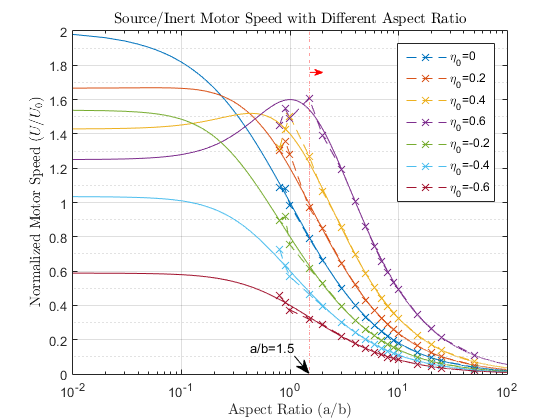
\includegraphics[width=\linewidth, height=4in]{2016-11-22-AnalyticVerification_Free.png}
\caption{Benchmark with analytic solution in free space}\label{2016-11-22-BWASIFS}
\end{figure}

\labday{Wednesday, 23 November 2016}
\experiment{Sixth Associated Group Meeting of Soft Matter, 2016 Autumn}
Title: Angiogenesis - Baby Retina Formation\\
Speaker: Yuankai Lu\\
Talked about some mechanism about blood vessels' generation. Not interested. I am more impressed with lecture in Zhiyuan Salon.\\
Title: Quantum Phase Transition, Magnetic Field, and Wilson Ratios\\
Speaker: Haiqing Lin, Beijing Computational Science Research Centre\\
Contents: Started from basic method and models of studying phase transition, such as Landau Theory of phase transition, XXZ model, etc. Also mentioned some Renormalization Group method. Many details are forgotten. Their recent work is about numerical simulation of quantum phase transition and made an effort to derive analytic expansion in finite temperature. Although there work agrees well with both numerical simulation and experiment data. That is not the part most impressive. They proposed a quantity, Wilson Ratio, to draw the phase diagram of targeted system. They showed the phase diagram drawn by Wilson Ratio which is clearly divided phase space into different phase region. Most importantly, these results are confirmed in different quantum system, like Fermi liquid, TLL, etc. \\
This lecture also talked about interesting experience of Wilson. Current academic environment is universally urgent. Researchers are always urgent for publication. The people like Wilson is rare in today's world. I need stay focused and do something meaningful in my PhD career.\\

Last, today's result are recorded below in Fig. \ref{2016-11-23-MSUCC}. I checked the motor speed under channel confinement. However, for larger aspect ratio, the limited channel length cannot be regarded as infinitely long , which causes a drop in motor speed.

\begin{figure}
\centering
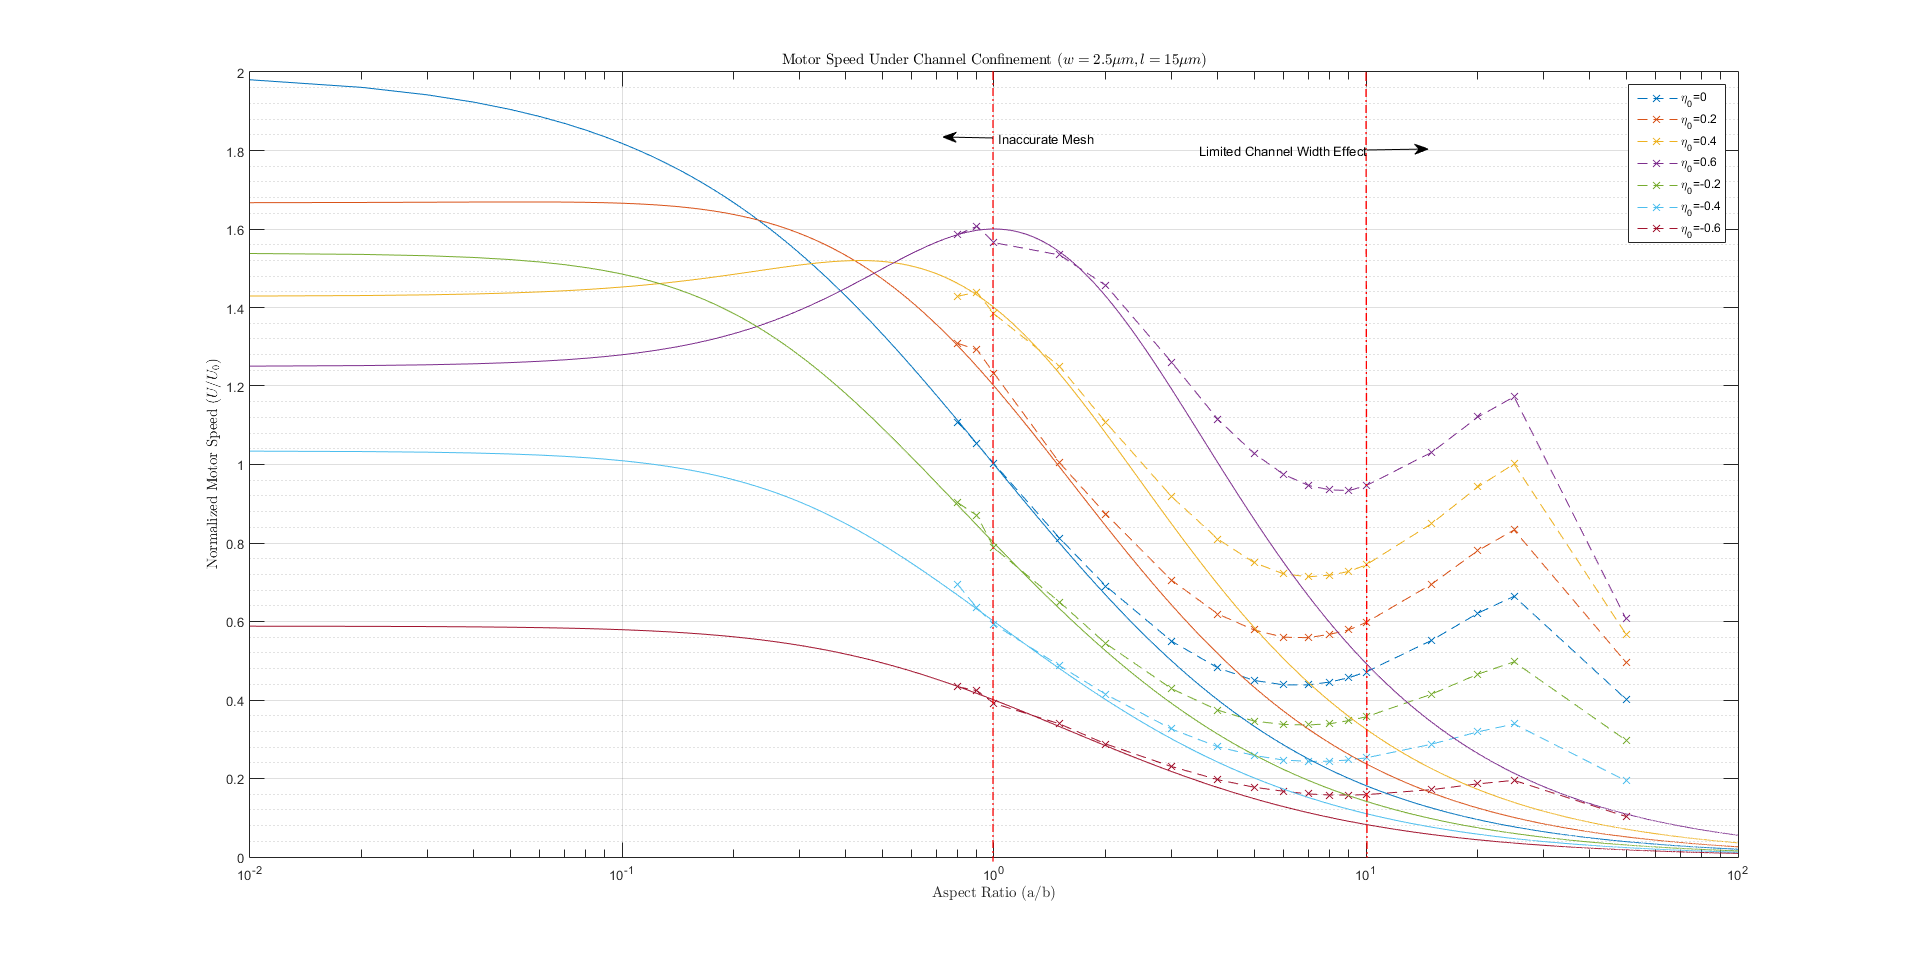
\includegraphics[width=\linewidth, height=3.5in]{2016-11-23-AnalyticVerification_Channel.png}
\caption{Motor Speed Under Channel Confinement. Solid lines are analytic results in free space.}\label{2016-11-23-MSUCC}
\end{figure}

\labday{Thursday, 24 November 2016}
In today's group meeting, Prof. Zhang mentioned a work about phototaxis bacteria in nature physics. This work designed a simple experiment: using laser to illuminate the center of bacteria medium. Then, bacteria will accumulate in the center because of phototaxis. An interesting phenomenon is there exists density fluctuation at the outer edge of center aggregation spot. This work claimed that these fluctuation was a wave. Thus, in the paper the author showed their explained with numerical simulation. A important concept used for explanation is bio-convection. Like the instability happened in the air-water interface, the layer formed by bacteria (because the bacteria used in paper preferred to stay in where shear stress is small) will be broken by periodic fluctuations. Prof. Zhang hoped to design a device to control bacteria to generate circular flow in macroscopic scale and proposed some ideas. \\
Today's numerical result is shown in Fig. \ref{2016-11-24-MSUDCC}. This figure shows the motor speed under different width of channel confinement. Results show that tighter confinement causes higher motor speed. Source/Inert motor indeed shows speed up although it's not too much. I have interests to derive these curves under confinement theoretically. Where to get started, I need to consider it more carefully.
\begin{figure}
\centering
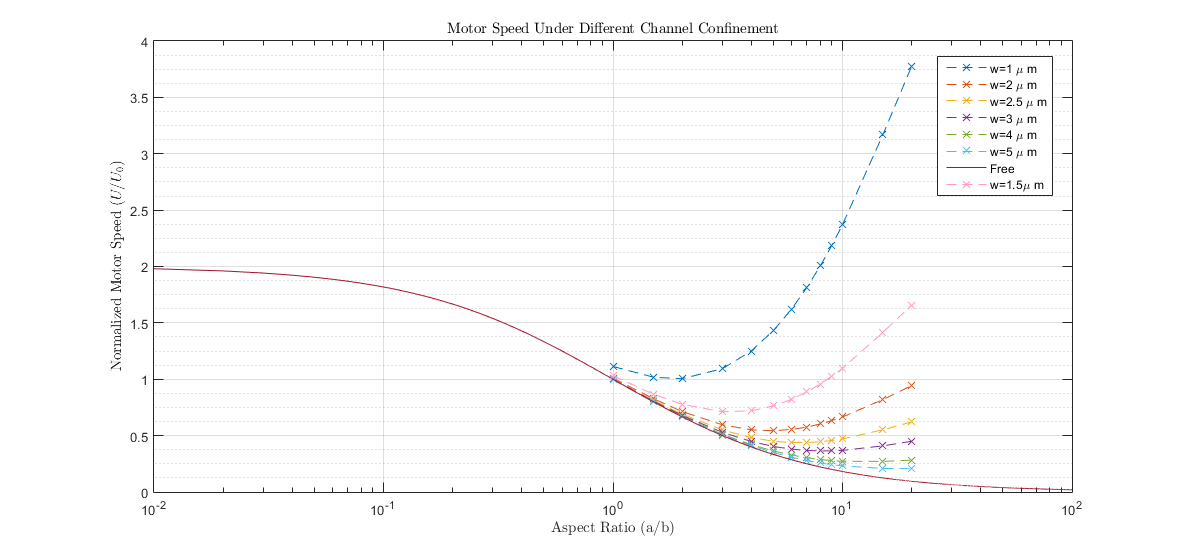
\includegraphics[width=\linewidth, height=3.5in]{2016-11-24-MotorSpeed_DiffChannel.png}
\caption{Motor Speed Under Different Channel Confinement [$\eta_0=0$] . Solid lines are analytic results in free space.}\label{2016-11-24-MSUDCC}
\end{figure}

\labday{Friday, 25 November 2016}
Today, I get my gre-physics score. Not too good. Just 86\% percentile and scaled score is 910. There is only one chance and now it's done. I have no choice but accept this score. I just wonder if I guess my unanswered questions I maybe get higher than 90\% percentile. Anyway, I have to admit that it affected my mood and I need to reconsider my PhD program. Good luck! While my research has to continue.\\

Today's results are following:
First, I check the effect caused by finite channel length which makes us cannot assume the channel wall as infinite large. Fig. \ref{2016-11-25-MSUDCC} confirm this effect and motor speed with large aspect doesn't drop down. I also compare it with previous result and Fig. \ref{2016-11-25-ECBFCE} shows clearly errors induced by finite channel length. That alerts me that I should pay close attention to parameters of channel which I usually do not care.
\begin{figure}
\centering
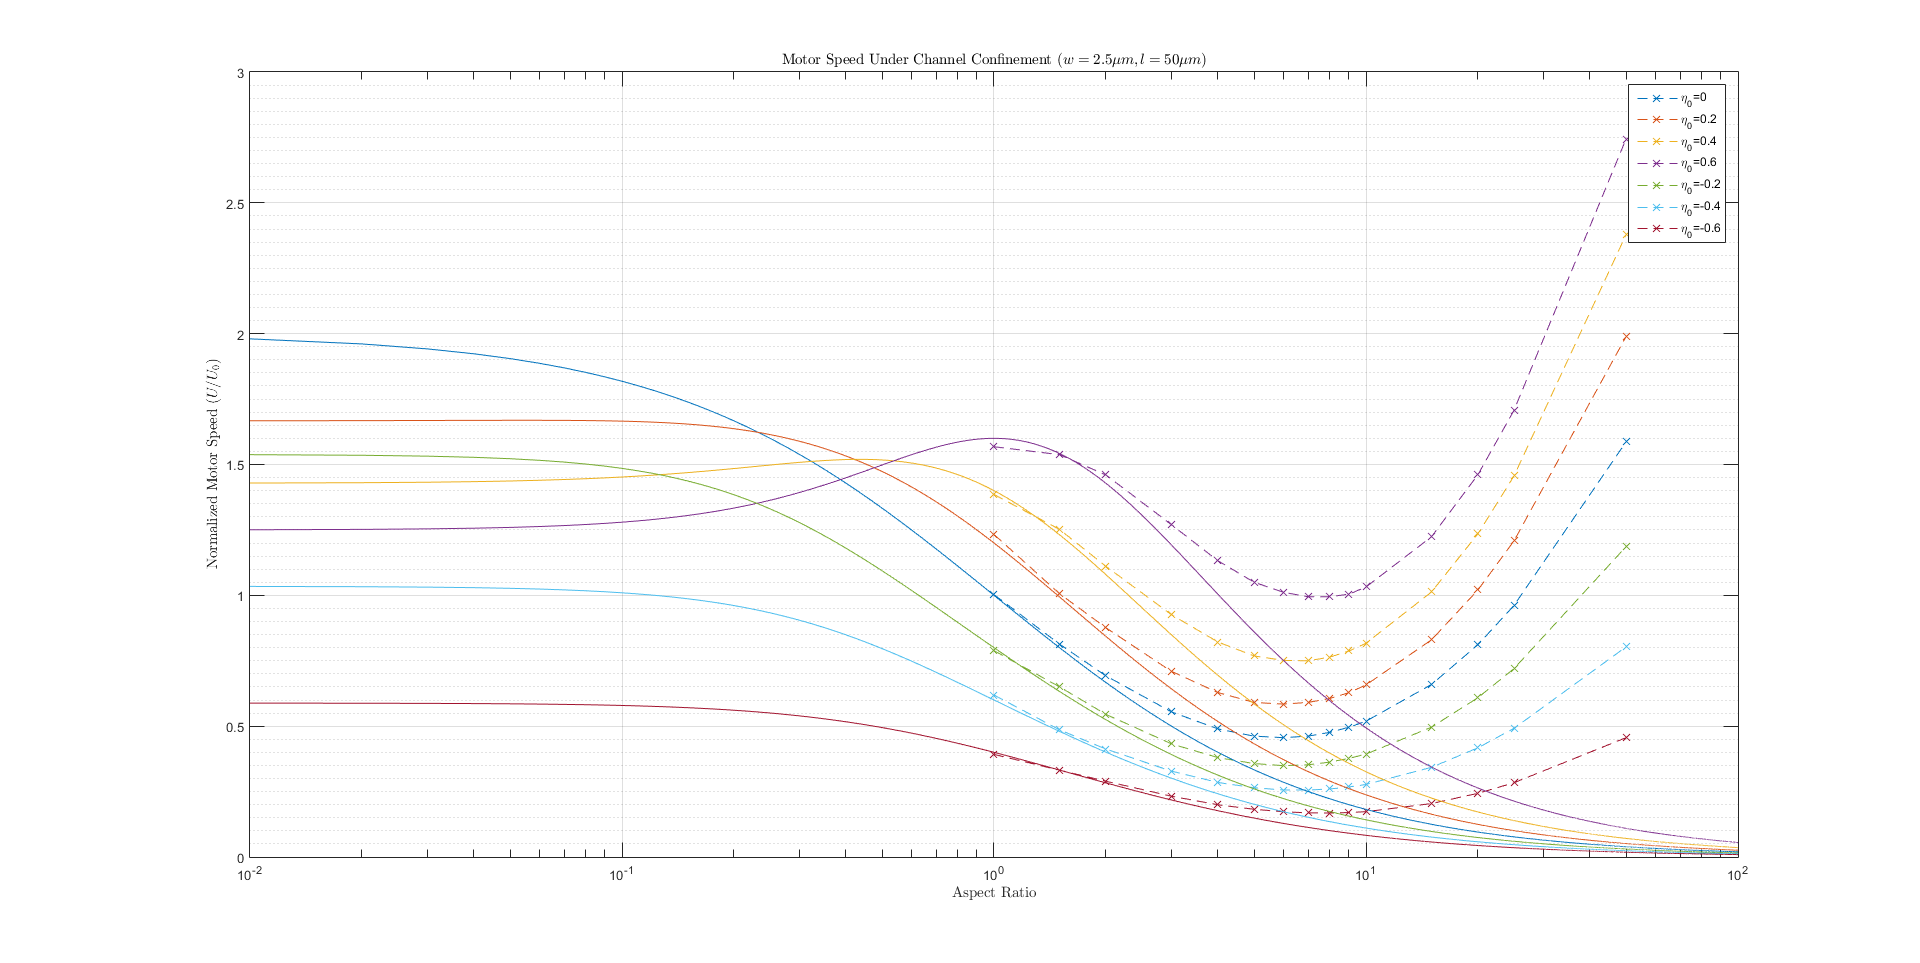
\includegraphics[width=\linewidth, height=3.5in]{2016-11-25-AnalyticVerification_Channel_New.png}
\caption{Motor Speed Under Different Channel Confinement [$\eta_0=0, w=50\mu m$] . Solid lines are analytic results in free space.}\label{2016-11-25-MSUDCC}
\end{figure}
\begin{figure}
\centering
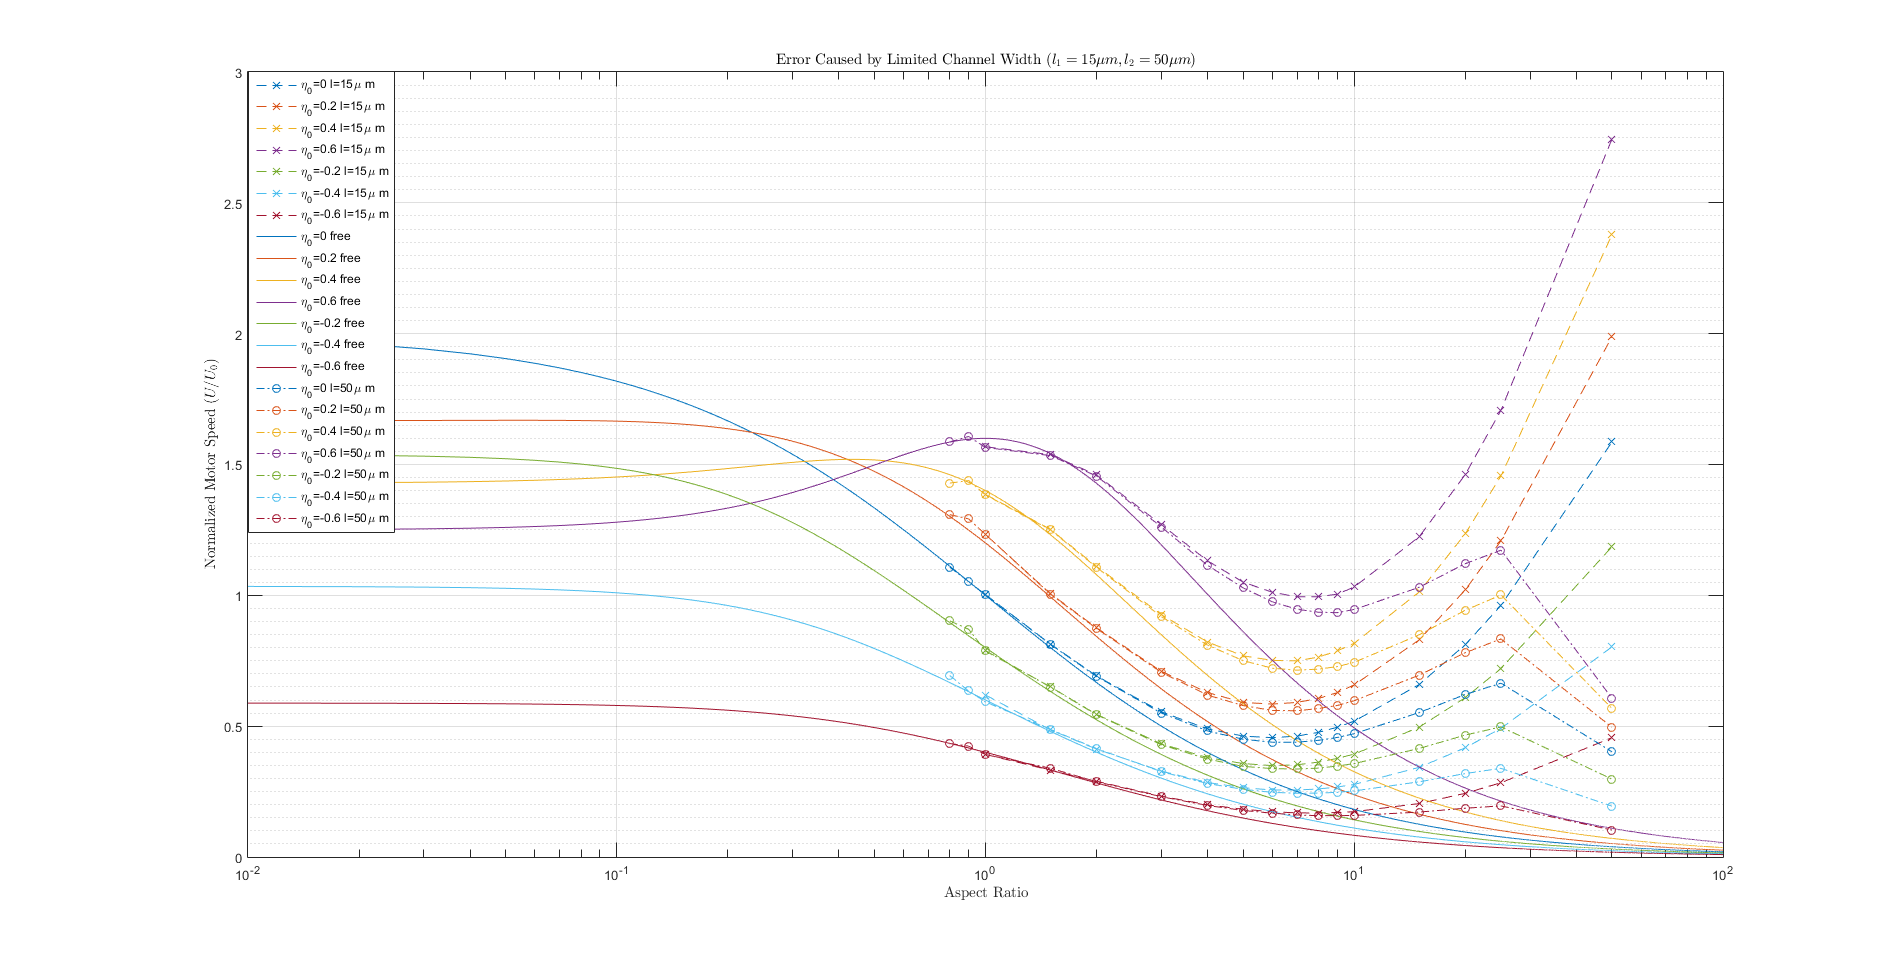
\includegraphics[width=\linewidth, height=3.5in]{2016-11-25-AnalyticVerification_Finite_Channel_Effect.png}
\caption{Error Caused by Finite Channel Effect [$\eta_0=0, w=15\mu m, 50\mu m$] . Solid lines are analytic results in free space.}\label{2016-11-25-ECBFCE}
\end{figure}

Then, I want to see how motor speed change under different channel width. Actually, I calculated these before. However, I want to look it more closely for my later theoretical work. Results are shown in Fig. \ref{2016-11-25-MSWDARL} and Fig. \ref{2016-11-25-MSWDARS}. There is one important feature. When channel width is large ($> 5\mu m$), motor speed approaches to speed in free space as expected and larger motor( which with larger aspect ratio) has lower motor speed in free space (because larger aspect ratio motor has larger surface area. Fluid field will cause larger resistant force to motors which have large surface). However, approximately (there are still some points violates following claim), larger motor display larger speed up under tight confinement while small motor speed up little. Intuitively, I think it makes sense because larger motor posses more charges which will generate large electrical field under tight confinement, in turn generate stronger electroosmotic flow and caused larger speed up. While, I do not have a quantitative description of this explanation. The fluid velocity field generated by source/inert motor is also different from source/sink motor. The next step, I plan to plot the velocity field of source/inert motor and compare it with source/sink motor. Via this, I hope to get a qualitative understanding of this problem firstly.
\begin{figure}
\centering
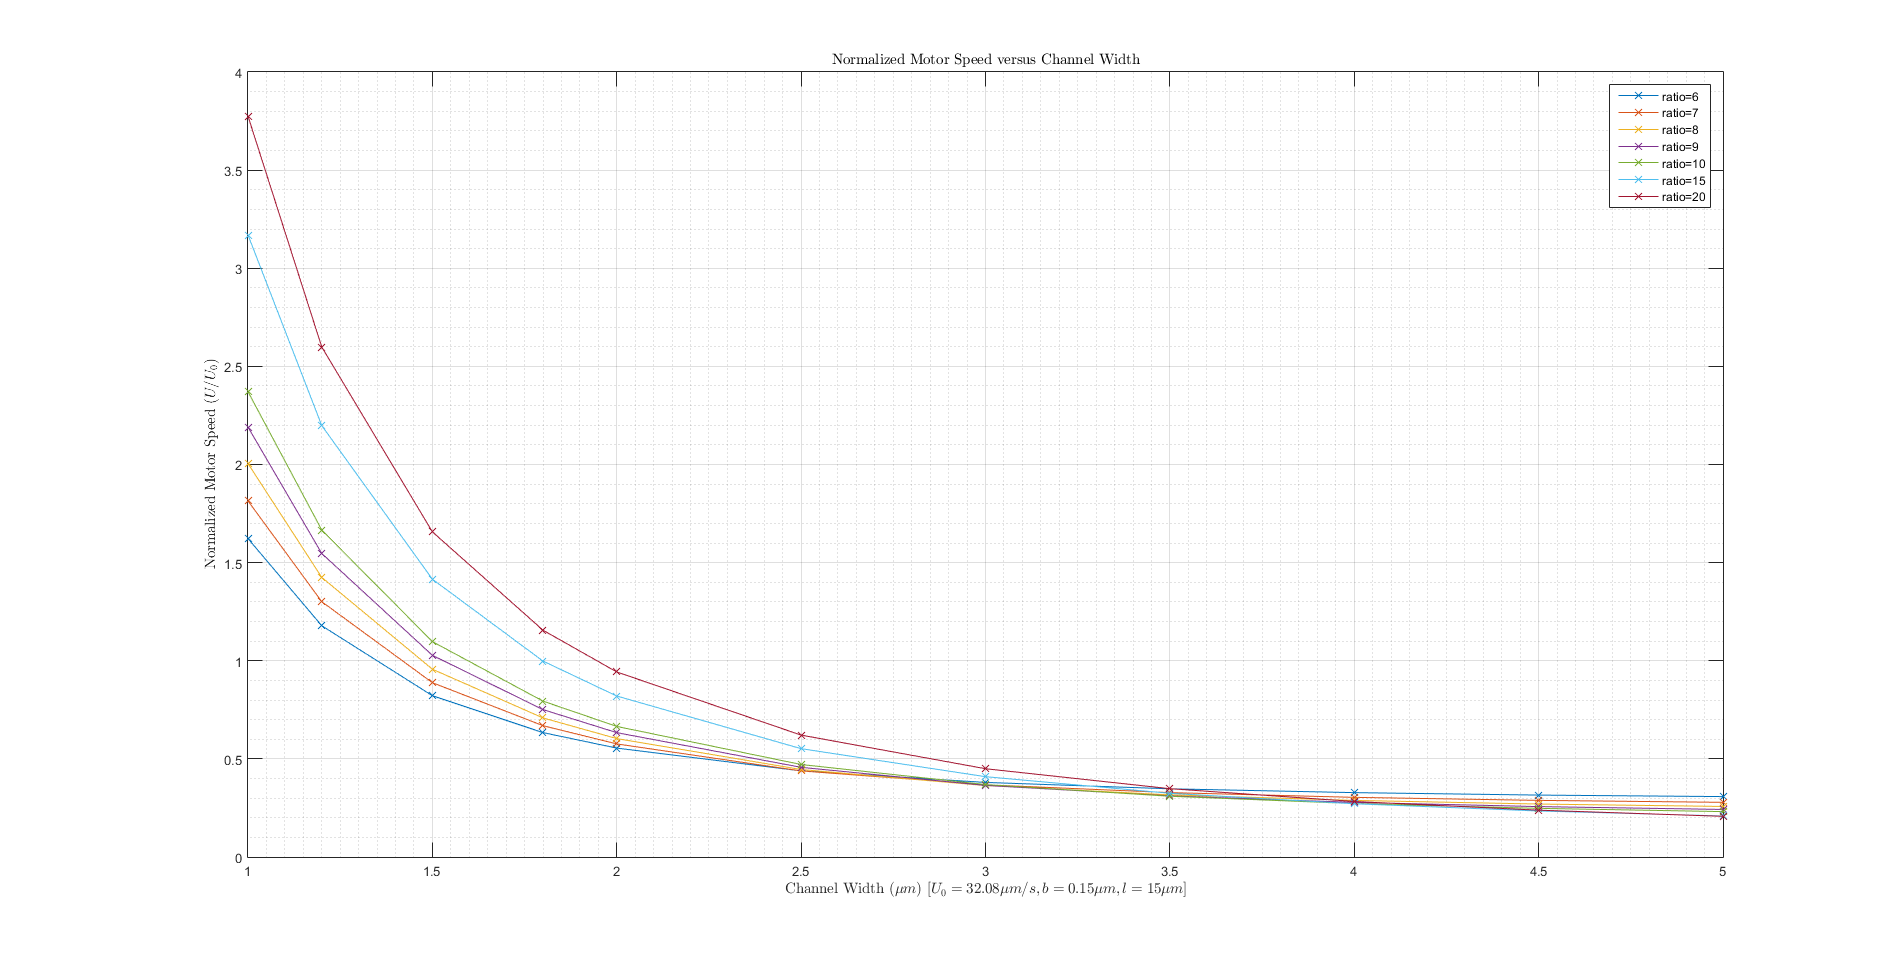
\includegraphics[width=\linewidth, height=3.5in]{2016-11-25-MotorSpeed_DiffCWidth_large.png}
\caption{Motor Speed With Different Aspect Ratio Under Differential Channel Confinement [$\eta_0=0, w=15\mu m$]}\label{2016-11-25-MSWDARL}
\end{figure}
\begin{figure}
\centering
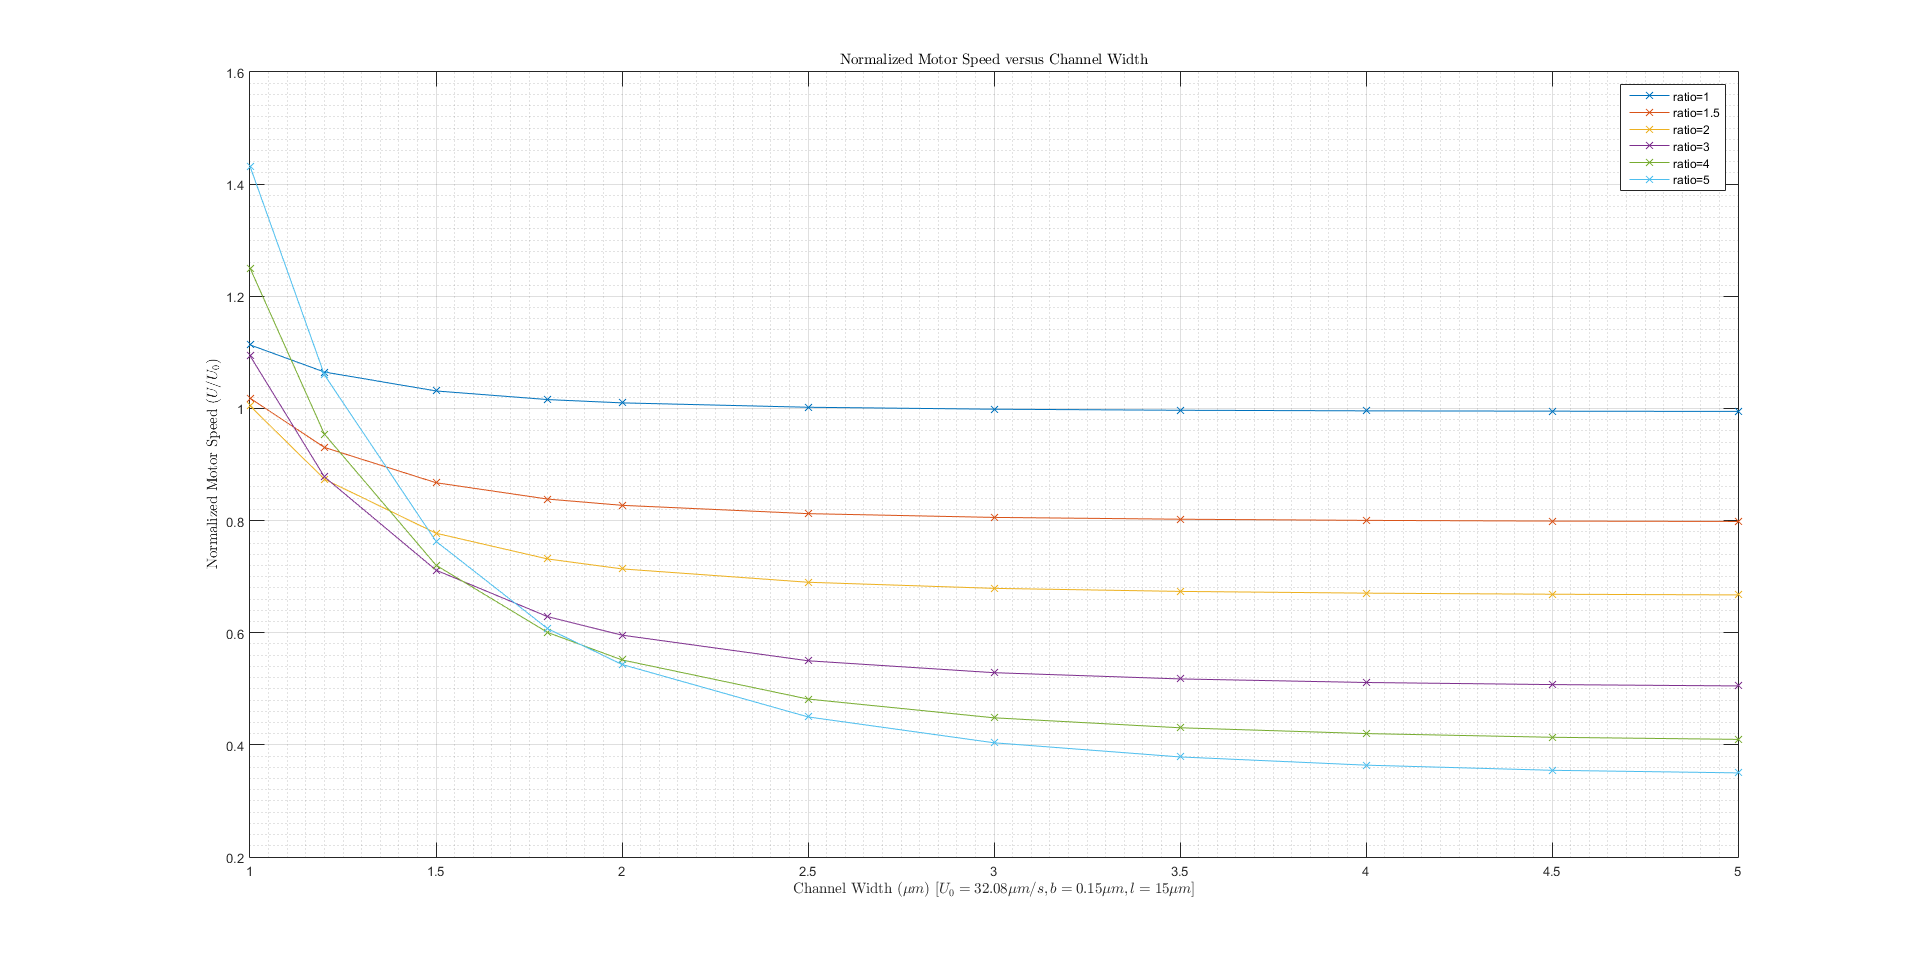
\includegraphics[width=\linewidth, height=3.5in]{2016-11-25-MotorSpeed_DiffCWidth_small.png}
\caption{Motor Speed With Different Aspect Ratio Under Differential Channel Confinement [$\eta_0=0, w=15\mu m$]}\label{2016-11-25-MSWDARS}
\end{figure}

\labday{Monday, 30 November 2016}
\experiment{Seventh Associated Group Meeting of Soft Matter, 2016 Autumn}
Title: Self-assembly of nonamphiphilic rod-like virus(es) in colloidal membrane\\
Abstract: The entropy-driven self-assembly of homogeneous rods into 2D colloidal membrane is similar to the assembly of lipids into ubiquitous biological membranes, despite the fact that lipid molecules are amphiphilic. In this talk, I will give an introduction of two experimental work on investigating the properties of the colloidal membranes.\\
Speaker: Huang, Chen\\
Today, Chen Huang delivers some contents about self-assembly of rod-like virus. His talk mainly concerns two papers. I am more interested in the second one\cite{Sharma2014}. In this paper, authors utilized two kind of virus, one is longer (approximately 1200 $nm$), another is shorter (approximately 800 $nm$). Interesting thing is these two viruses have different chiralities. Each of these viruses will form a monolayer membrane in depletan solvent. When two membrane merged together, the combined system will display different kinds of phase separation. When the concentration of solvent is low, shorter viruses will mix homogeneously with longer viruses. When the concentration is high, shorter viruses will form a large cluster within longer viruses membrane. However, when the concentration is intermediate, shorter viruses form lots  of clusters, which are called rafts, floated within longer viruses membrane. Besides, these rafts structure are thermodynamically stable. Initially connect by "dynamical bridges", then form rather homogeneous rafts with approximate the same radius size. By adjusting the concentration of solvent, the interactions between rafts could be effectively attractive. In this case, some special polymer structure could be formed rather stably (up to several days).\\
The role of chirality plays in this experiment is not fully understood. Unlike our bio-membrane which has only one chirality molecule - cholesterol, there are two kind of viruses with opposite chiralities. Whether this difference is essential, it is still unclear.
%----------------------------------------------------------------------------------------

\labday{Monday, 5 December 2016}
Last week, because of the final examination of Latin course, mid-term examination of differential geometry and some other meticulous stuffs about PhD application, I suspended my research. That really makes feel guilty. The most important thing is I found suspending other things and concentrated on only one thing cannot let me do things better! Therefore, I decide to recover my research and learning progress although the next week will be the busiest week for PhD application. In the forthcoming week, the day time belongs to learning and research, the night time belongs to application. The final week of application, I have to arrange everything nice and clearly. Then I will be free from application affairs. \\
Let me come back to research. I met a bottle neck in my current research. Until now, I have understood technical problems well. However, to move forwards, I have to strengthen my theoretical aspect. Currently, I want to check the possibility of calculating the motor speed up analytically. It might be difficult but my current model system is totally linear. I still have some confidence. To begin with, I want to read the review paper of Anderson\cite{Anderson1989}.
\experiment{Paper000021}
In the first reading of this paper, I did not grasp the essence. I need to reread this paper again in later time. Here I list some impressed information I obtained from this paper:
\begin{enumerate}
\item
charged particle plus its counterion cloud display as neutral in the region beyond Debye length. However, it still could move under external electric field because it's not rigid. The velocity field within interfacial region is crucial for determining the motion of particle. 
\item
A very important notion about interfacial transport phenomena is slip velocity
\item
When the boundary conditions are prescribed as slip velocity, the velocity field in outer region could be described by a potential flow. Decayed as $\frac{1}{r^3}$. 
\item
The boundary effect could speed up the electrophoresis. However, the speed up is only significant when the distance between wall and particle is comparable with particle radius. The results show that particle speed up about $25\%$ more when $h/a \approx 0.995$. This kind of speed up is much weaker than the speed up found in my current work about bimetallic motor. It seems localized electroosmostic flow could generate much stronger localized gradient of electrical potential under channel confinement.
\item
Above statement may imply that my hope to apply previous work directly will be difficult. Electroosmostic flow and localized electroosmostic flow should be studied in more detail.
\end{enumerate}
\labday{Monday, 12 December 2016}
\experiment{Workshop on Soft Matter Sciences}
\large{Brief Introduction}\\
The soft matter physics group at Shanghai Jiao Tong University (SJTU) is organizing an international workshop on Soft Matter Sciences in December 12-14, 2016. The main purpose of this workshop is to celebrate the inauguration of the Center for Soft Matter and Interdisciplinary Sciences at SJTU. The workshop aims to bring together a number of outstanding scientists in soft matter and related fields, to facilitate exchange of ideas and results, and to nurture interdisciplinary collaborations. The workshop will consist of two and half days of informal talks, along with ample time for discussions.
\large{Brief Recording}
It's pretty lucky to have a chance to take part in this workshop. After taking part in many group meeting in soft matter physics, I have been relatively familiar with works proceeding in SJTU. Through this workshop, I could appreciate how other groups in soft condensed matter physics in the world are doing. Of course, it's my first time to hear lectures given by top scholars in this field, such as David Weitz, Paul Chaikin, etc. Their talks are very impressive and their works are really brilliant. I can see the distance between our works and the first-class work in the world. However, I also feel fortune that I study in SJTU and do researches related to soft matter because I do feel my teachers' passion and our groups' vitality, which,at least for me, is much more important.\\
Another impressive memory is the poster section in Dec. 15, 2016. We several undergraduate could have a chance to pretend as a PhD student to explain our work. This feels good. Of course, we also enjoyed a great meal at that night.

\labday{Sunday, 18 December 2016}
\experiment{A Comparison Between Source/Sink Motor and Source/Inert Motor}
My PhD applications affairs are finally done. I have done everything I can do. The rest is not controlled by me. Best wishes to my PhD application. Now I can concentrate on my thesis work. After a brief discussion with Prof. Zhang, I will summarize my previous works firstly. Here I will present a systematic comparison between source/sink motor and source/inert motor.\\

\begin{enumerate}
\item \textbf{Benchmark numerical model in COMSOL}\\
\begin{itemize}
\item Source/Sink Fig. \ref{2016-12-18-BSSMM}
\item Source/Inert Fig. \ref{2016-12-18-BSIMM}
\begin{figure}
\centering
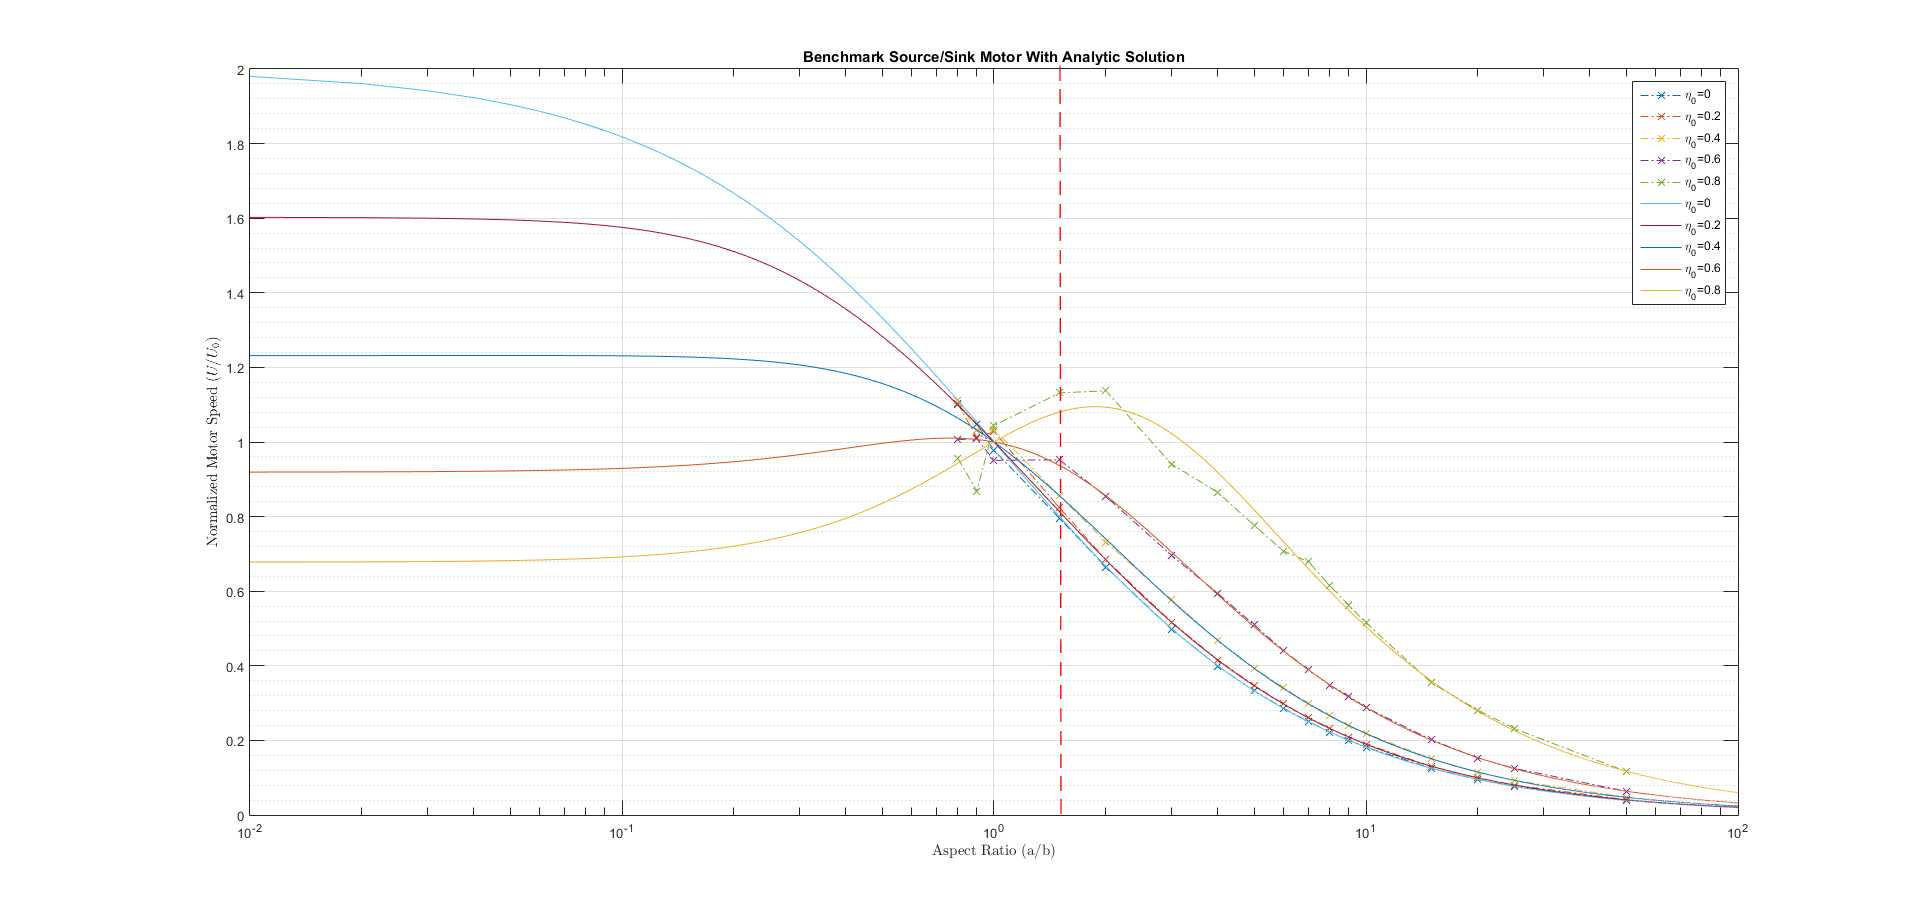
\includegraphics[width=\linewidth, height=3.5in]{2016-12-25-Benchmark_SourceSink_Free.png}
\caption{Benchmark of Source/Sink Motor Model}\label{2016-12-18-BSSMM}
\end{figure}
\begin{figure}
\centering
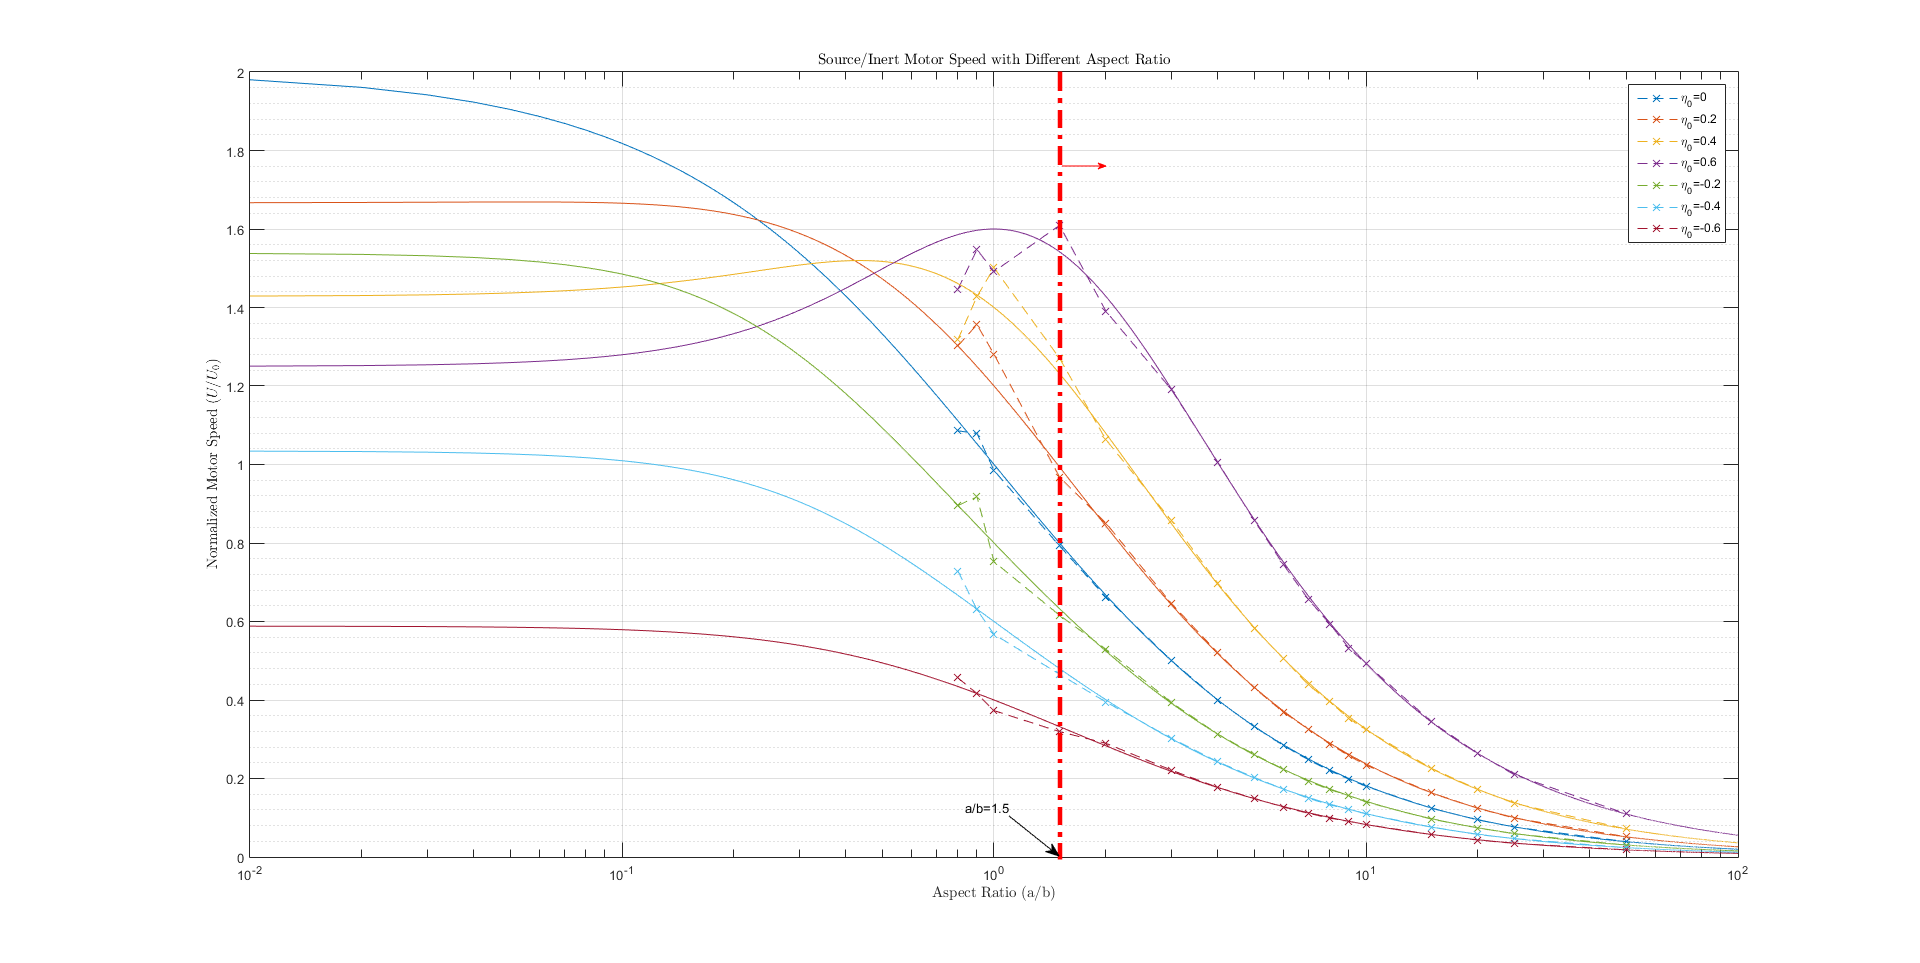
\includegraphics[width=\linewidth, height=3.5in]{2016-12-18-Benchmark_SourceInert_Free.png}
\caption{Benchmark of Source/Inert Motor Model}\label{2016-12-18-BSIMM}
\end{figure}
\end{itemize}
\item \textbf{Motor speed versus aspect ratio under channel confinement (fixed channel width)}\\
\begin{itemize}
\item Source/Sink Fig. \ref{2016-12-25-SSMSCUFCW}
\item Source/Inert Fig. \ref{2016-12-18-SIMSCUFCW}
\begin{figure}
\centering
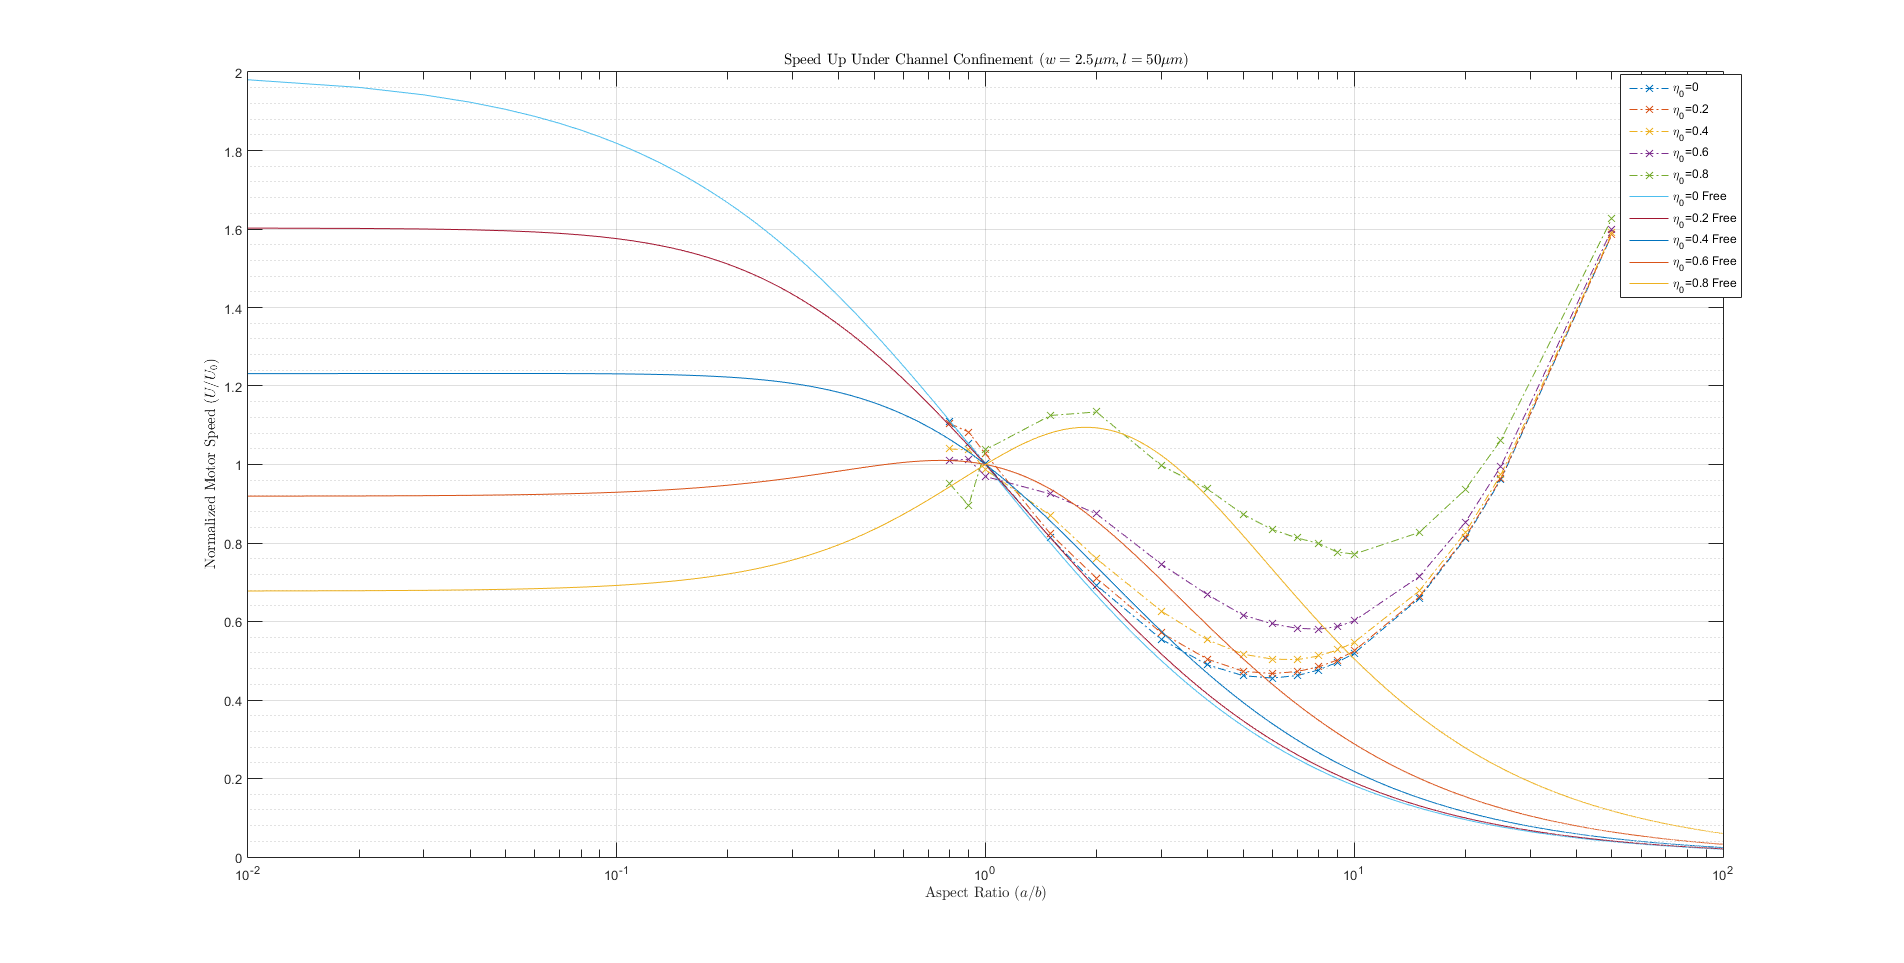
\includegraphics[width=\linewidth, height=3.5in]{2016-12-25-Ratio_SourceSink_Channel.png}
\caption{Source/Sink Motor Speed Change Under Fixed Channel Width}\label{2016-12-25-SSMSCUFCW}
\end{figure}
\begin{figure}
\centering
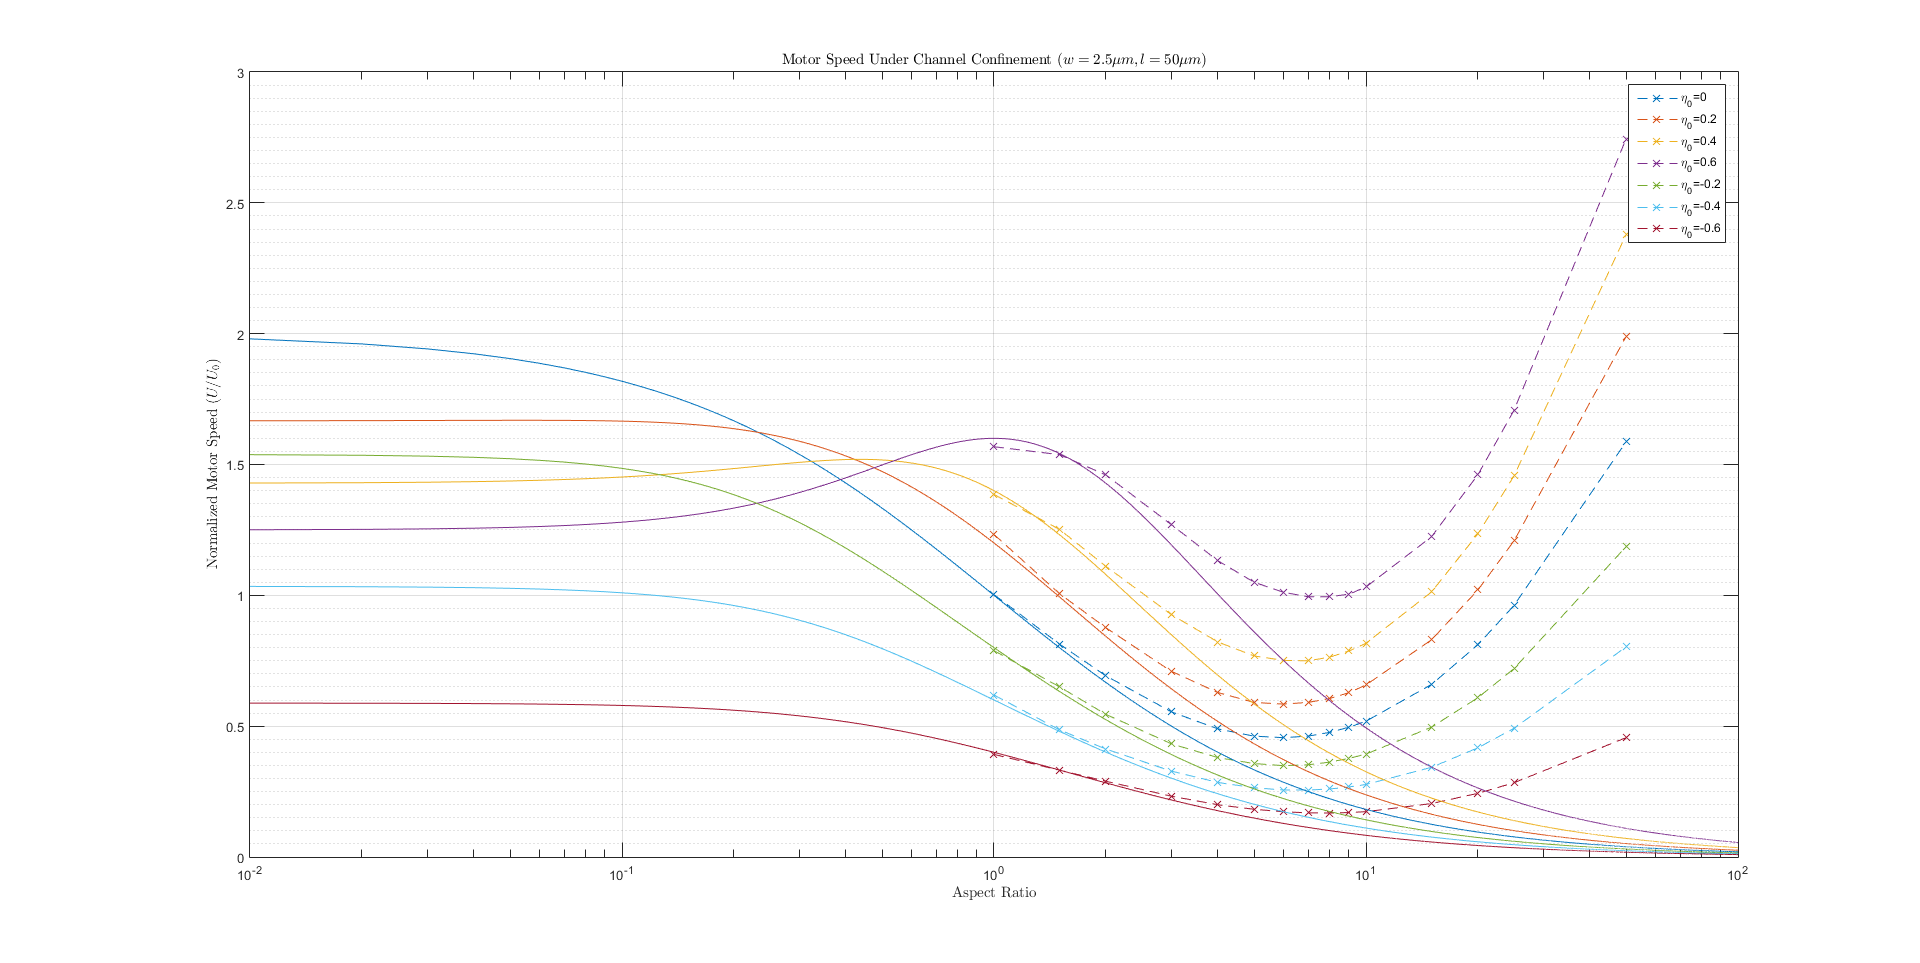
\includegraphics[width=\linewidth, height=3.5in]{2016-12-18-Ratio_SourceInert_Channel.png}
\caption{Source/Inert Motor Speed Change Under Fixed Channel Width}\label{2016-12-18-SIMSCUFCW}
\end{figure}
\end{itemize}
\item \textbf{Motor speed versus aspect ratio under different channel confinement (fixed $\eta_0$)}\\
\begin{itemize}
\item Source/Sink $\eta_0=0.2$ Fig.\ref{2016-12-25-SSMSCUDCC2} $\eta_0=0$ Fig. \ref{2016-12-25-SSMSCUDCC0}
\item Source/Inert Fig. \ref{2016-12-18-SIMSCUDCC}

\begin{figure}
\centering
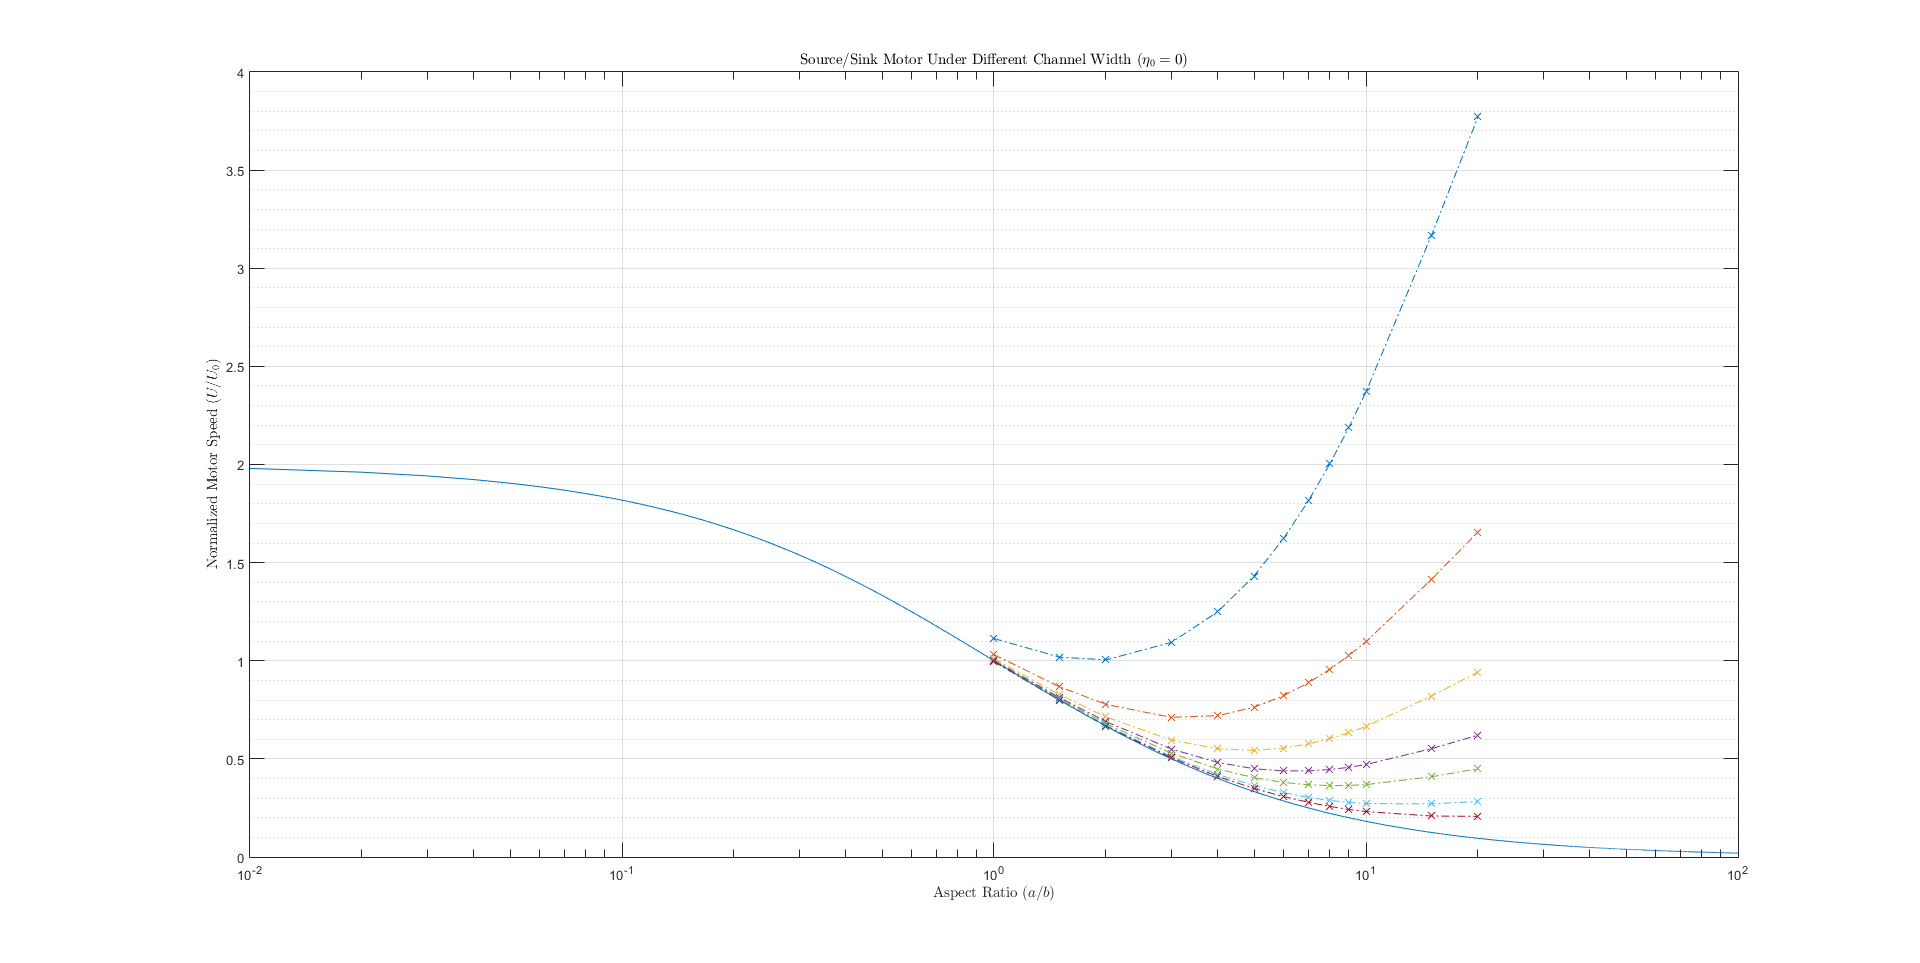
\includegraphics[width=\linewidth, height=3.5in]{2016-12-26-DiffChannel_SourceSink_eta0.png}
\caption{Source/Sink Motor Speed Change Under Different Channel Confinement}\label{2016-12-25-SSMSCUDCC0}
\end{figure}
\begin{figure}
\centering
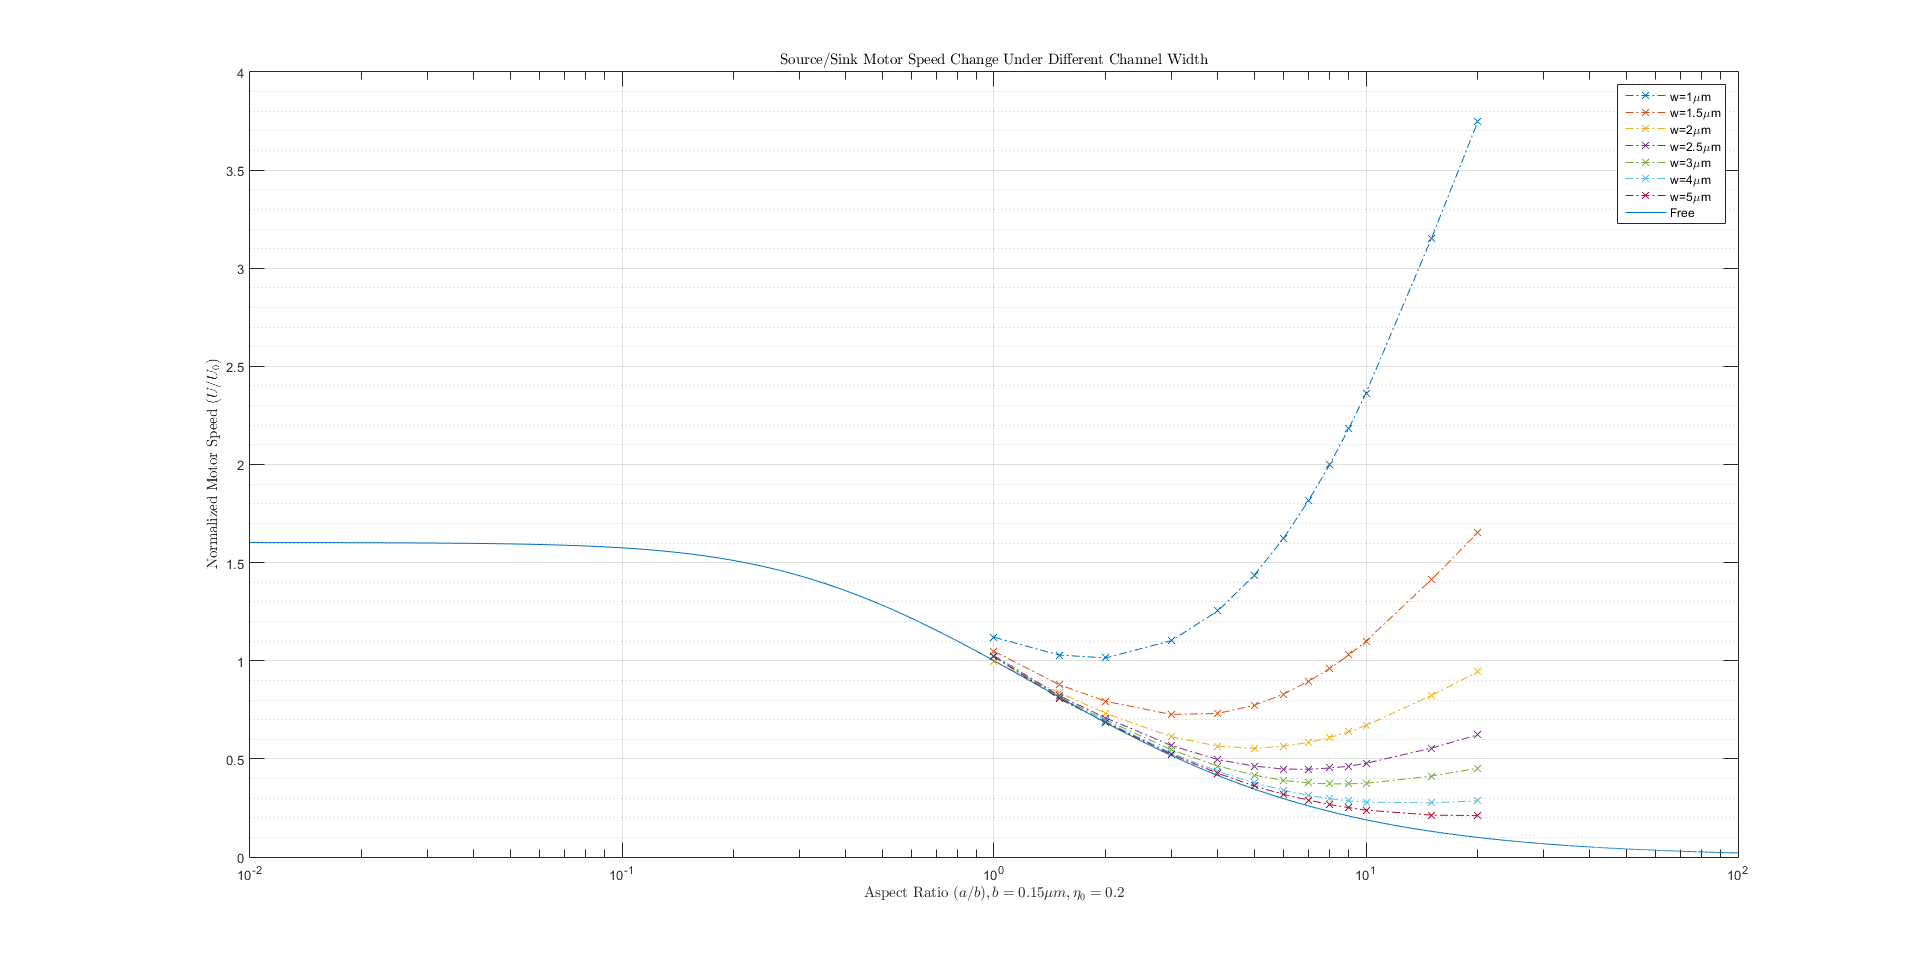
\includegraphics[width=\linewidth, height=3.5in]{2016-12-25-DiffChannel_SourceSink_eta02.png}
\caption{Source/Sink Motor Speed Change Under Different Channel Confinement}\label{2016-12-25-SSMSCUDCC2}
\end{figure}
\begin{figure}
\centering
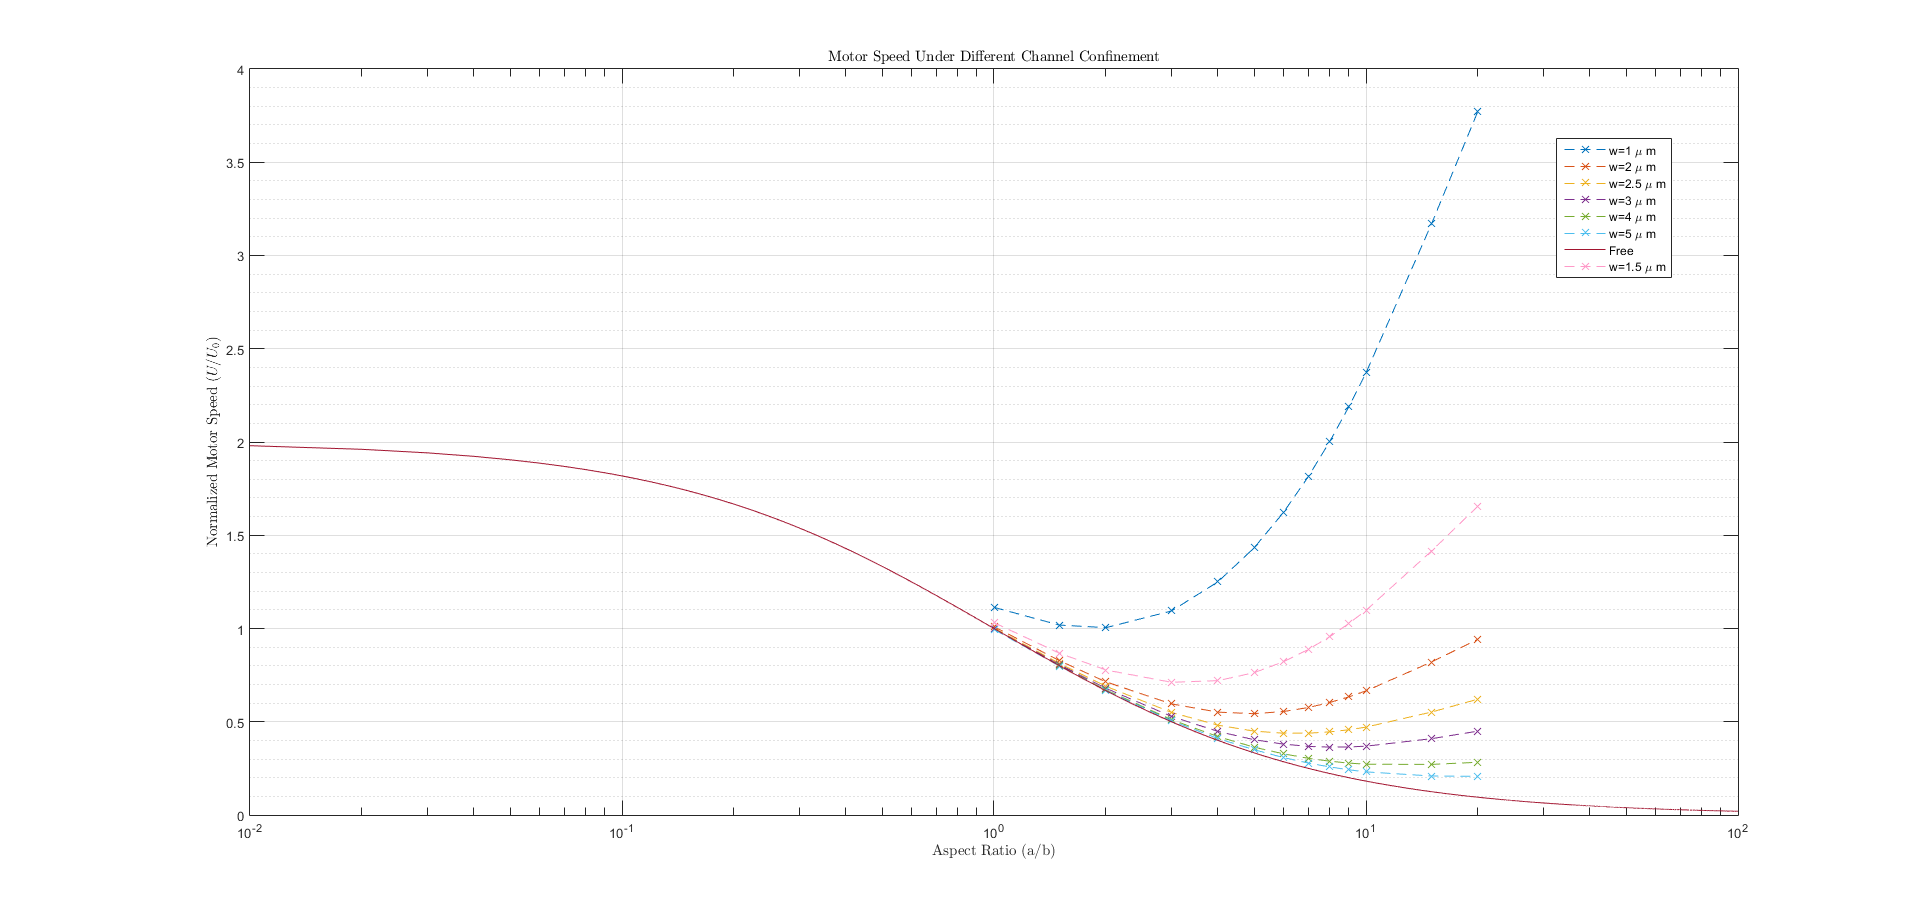
\includegraphics[width=\linewidth, height=3.5in]{2016-12-18-DiffChannel_SourceInert_eta0.png}
\caption{Source/Inert Motor Speed Change Under Different Channel Confinement}\label{2016-12-18-SIMSCUDCC}
\end{figure}
\end{itemize}
\item \textbf{Motor speed versus different channel width (fixed motor geometry)}\\
\begin{itemize}
\item Source/Sink Fig. \ref{2016-12-25-SSMSCUDCW}
\item Source/Inert Fig. \ref{2016-12-25-SIMSCUDCW}
\begin{figure}
\centering
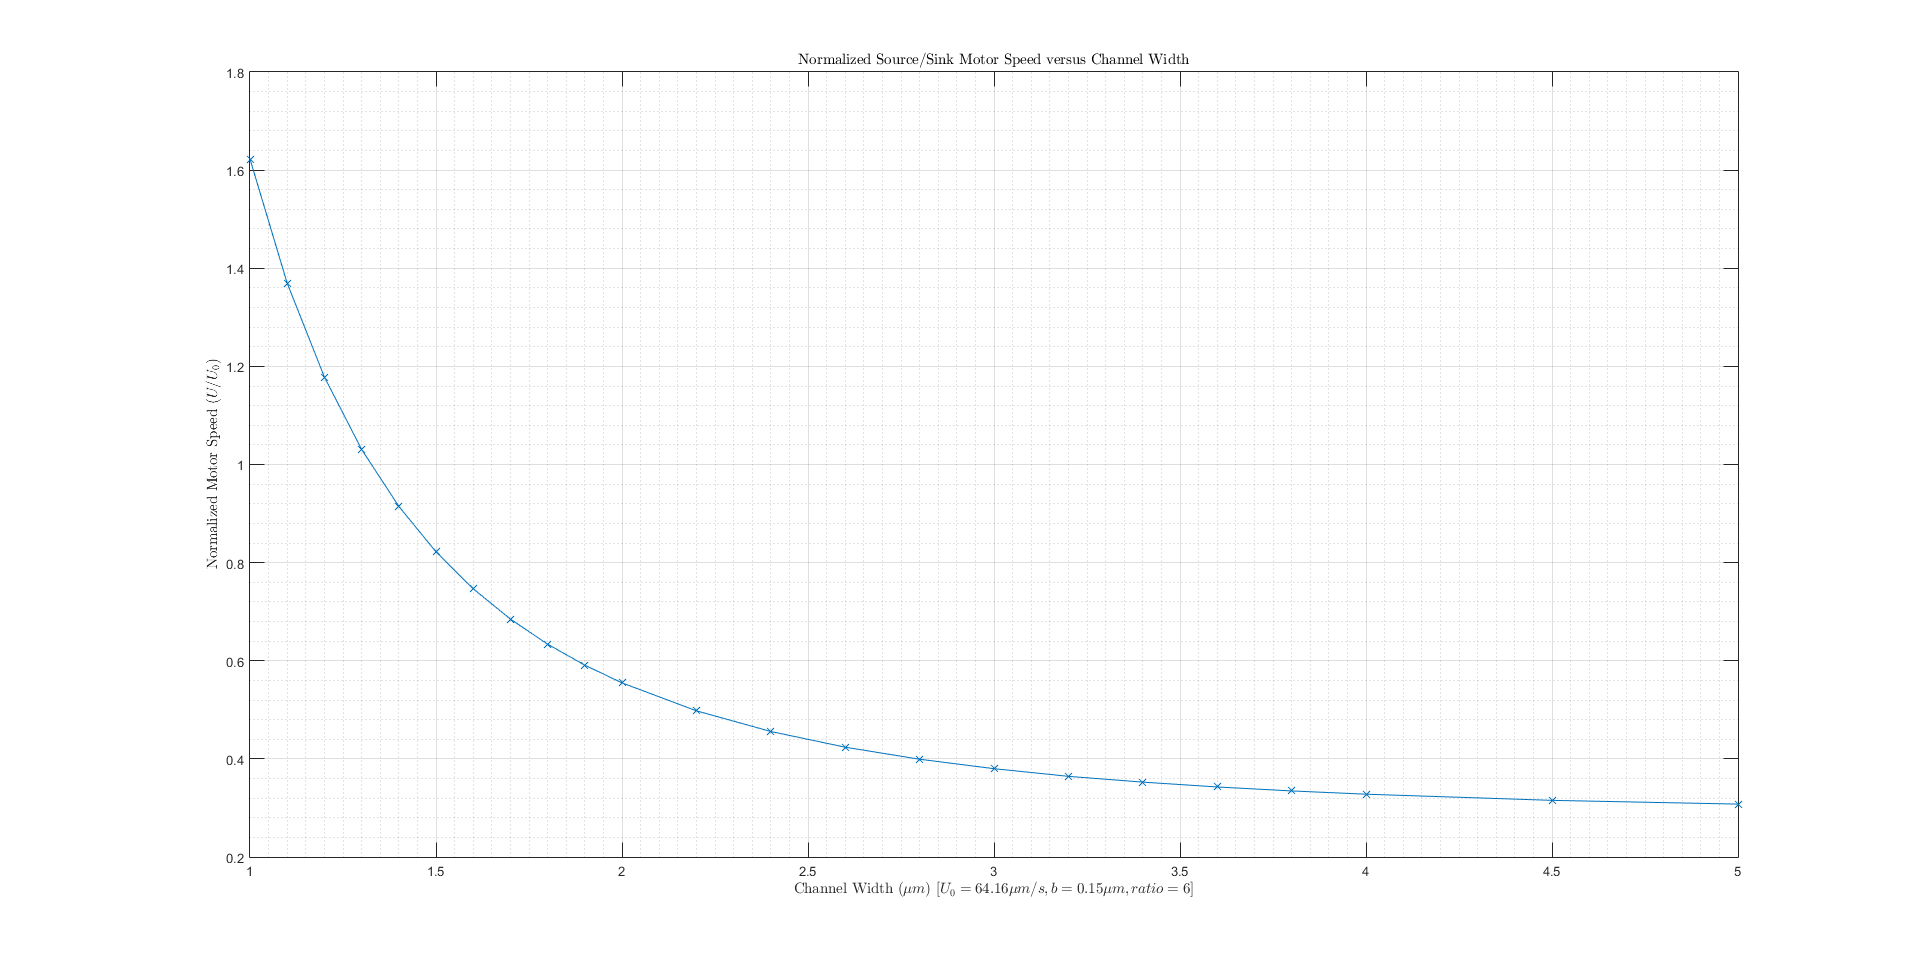
\includegraphics[width=\linewidth, height=3.5in]{2016-12-25-Speed_Diff_CWidth_SourceSink.png}
\caption{Source/Sink Motor Speed Change Under Different Channel Width (fixed motor geometry)}\label{2016-12-25-SSMSCUDCW}
\end{figure}
\begin{figure}
\centering
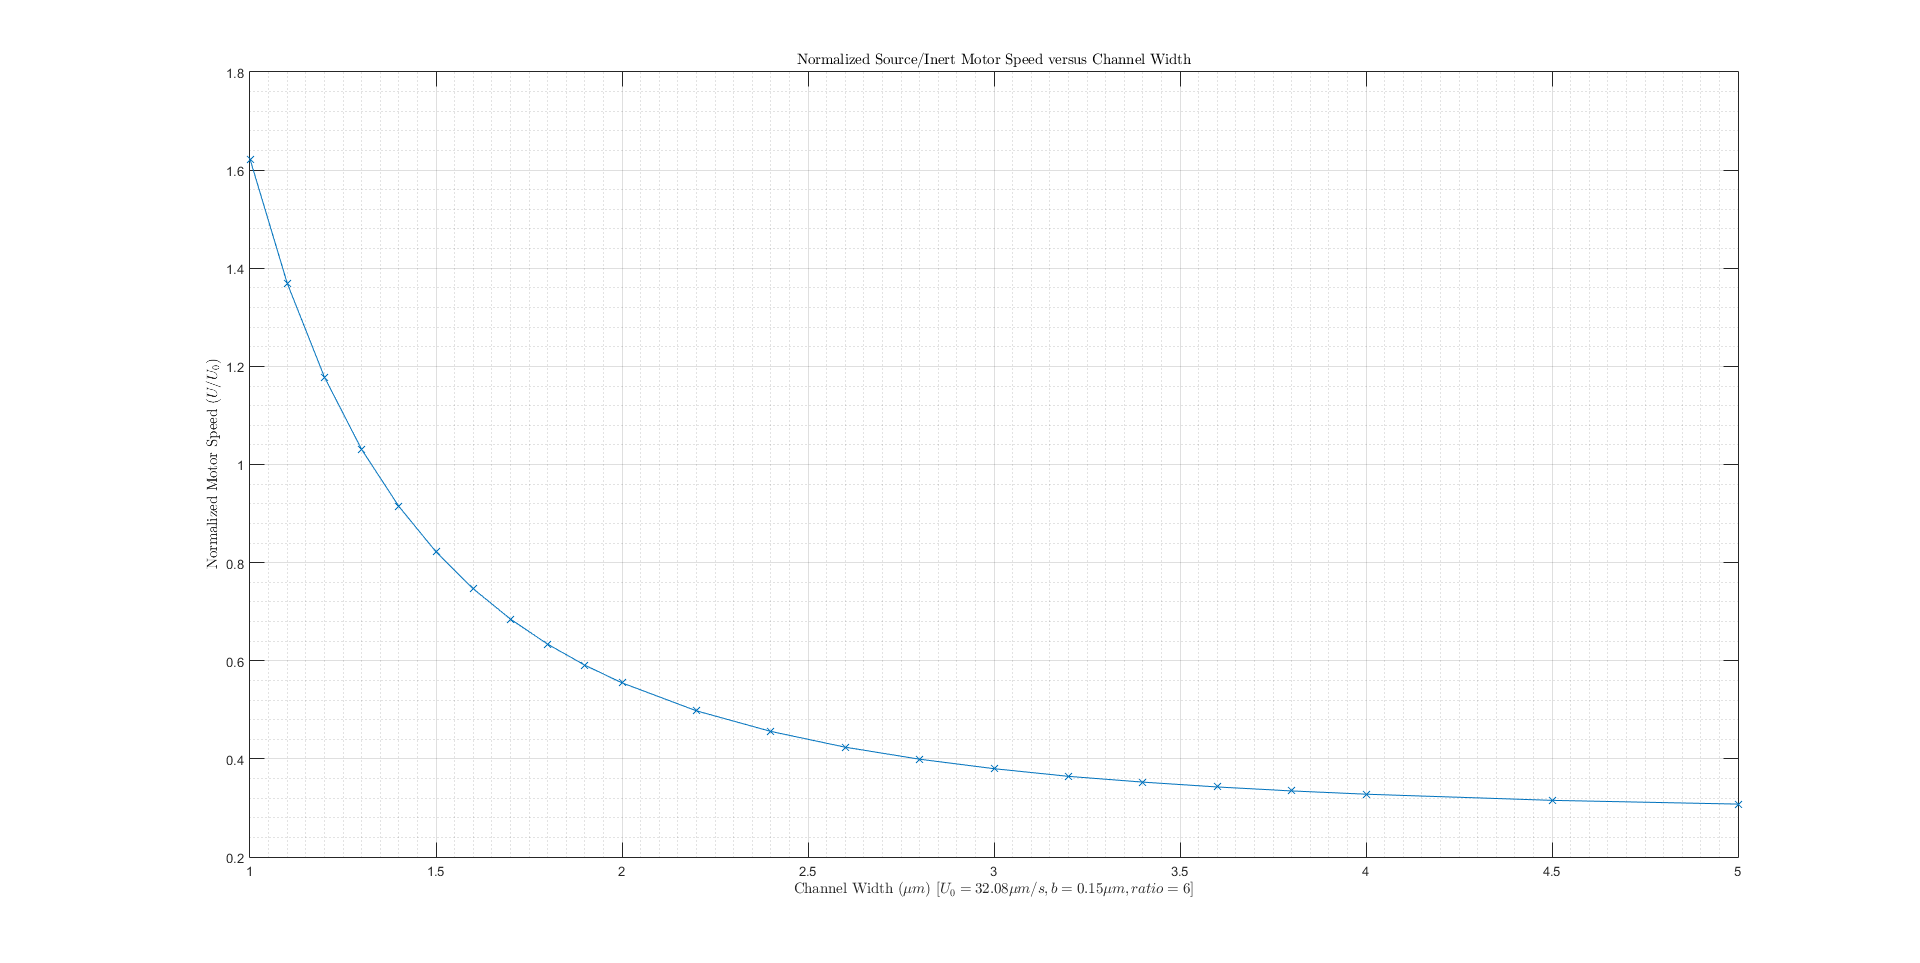
\includegraphics[width=\linewidth, height=3.5in]{2016-12-25-Speed_Diff_CWidth_SourceInert.png}
\caption{Source/Inert Motor Speed Change Under Different Channel Width (fixed motor geometry)}\label{2016-12-25-SIMSCUDCW}
\end{figure}
\end{itemize}
\item \textbf{Electric Field Generated by motor}\\
\begin{itemize}
\item Source/Sink Fig. \ref{2016-12-18-TLEFGBSSM}
\begin{figure}
\centering
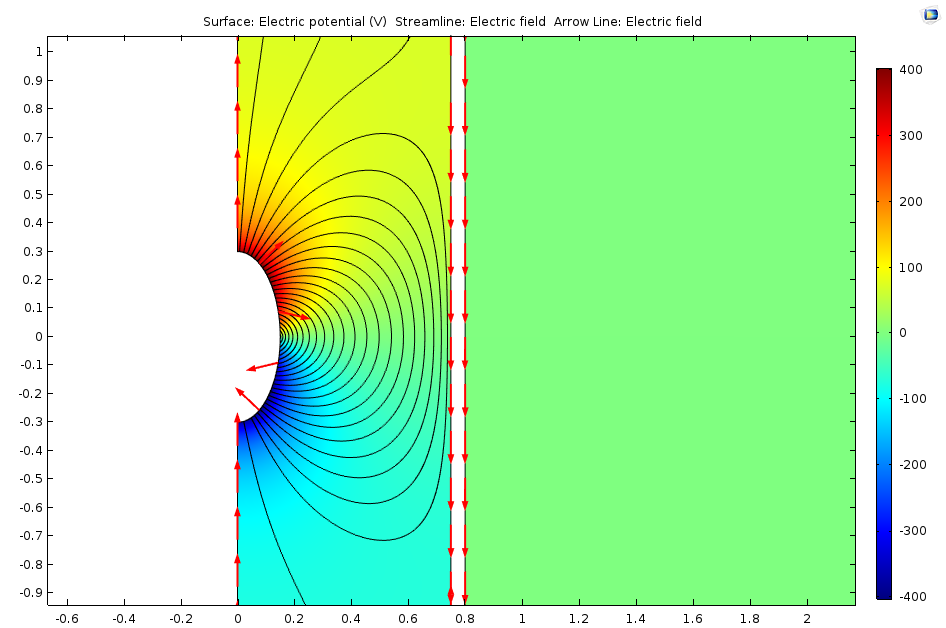
\includegraphics[width=\linewidth, height=3.5in]{2016-12-18-SourceSink-E.png}
\caption{Typical Localized Electrical Field Generated By Source/Sink Motor}\label{2016-12-18-TLEFGBSSM}
\end{figure}
\item Source/Inert Fig. \ref{2016-12-18-TLEFGBSIM}
\begin{figure}
\centering
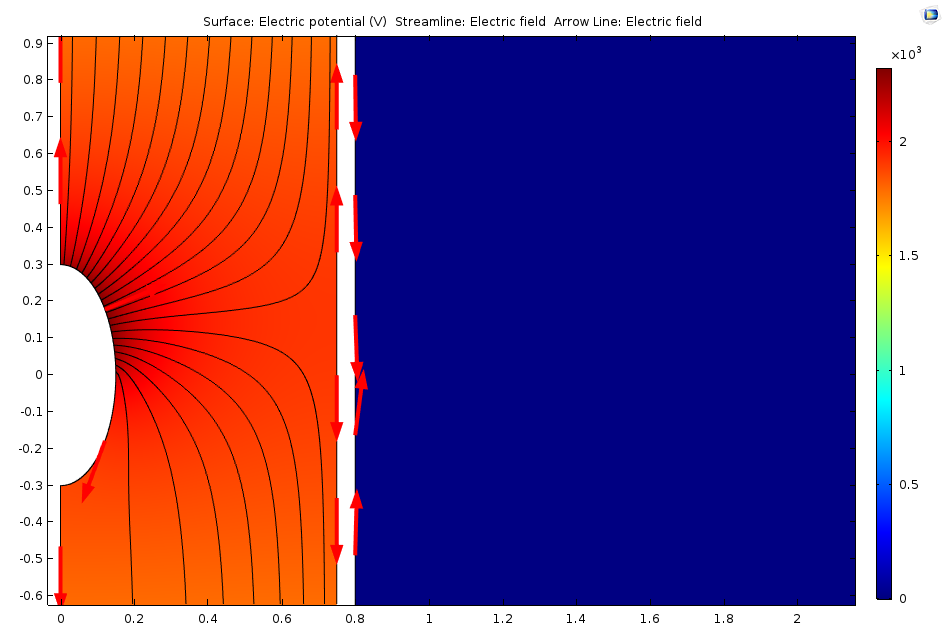
\includegraphics[width=\linewidth, height=3.5in]{2016-12-18-SourceInert-E.png}
\caption{Typical Localized Electrical Field Generated By Source/Inert Motor}\label{2016-12-18-TLEFGBSIM}
\end{figure}
\end{itemize}
\item \textbf{Fluid Field Generated by motor}\\
\begin{itemize}
\item Source/Sink Fig. \ref{2016-12-18-TLFFGBSSM}
\begin{figure}
\centering
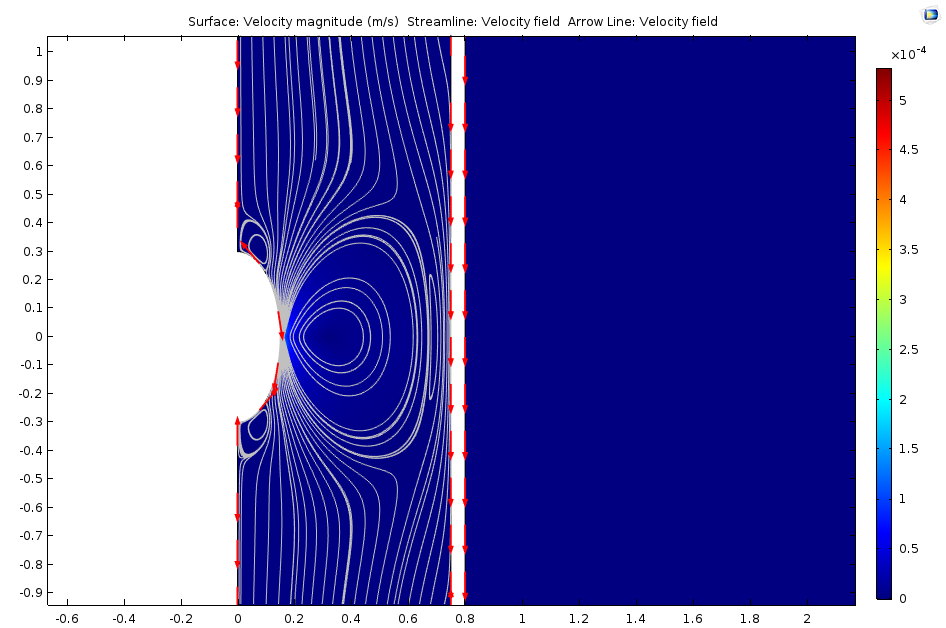
\includegraphics[width=\linewidth, height=3.5in]{2016-12-18-SourceSink-V.png}
\caption{Typical Localized Fluid Field Generated By Source/Sink Motor}\label{2016-12-18-TLFFGBSSM}
\end{figure}
\item Source/Inert In Progress
\end{itemize}
\item \textbf{Influence of Motor Shape}\\
Fig. \ref{2016-12-18-CBSMARM}
\begin{figure}
\centering
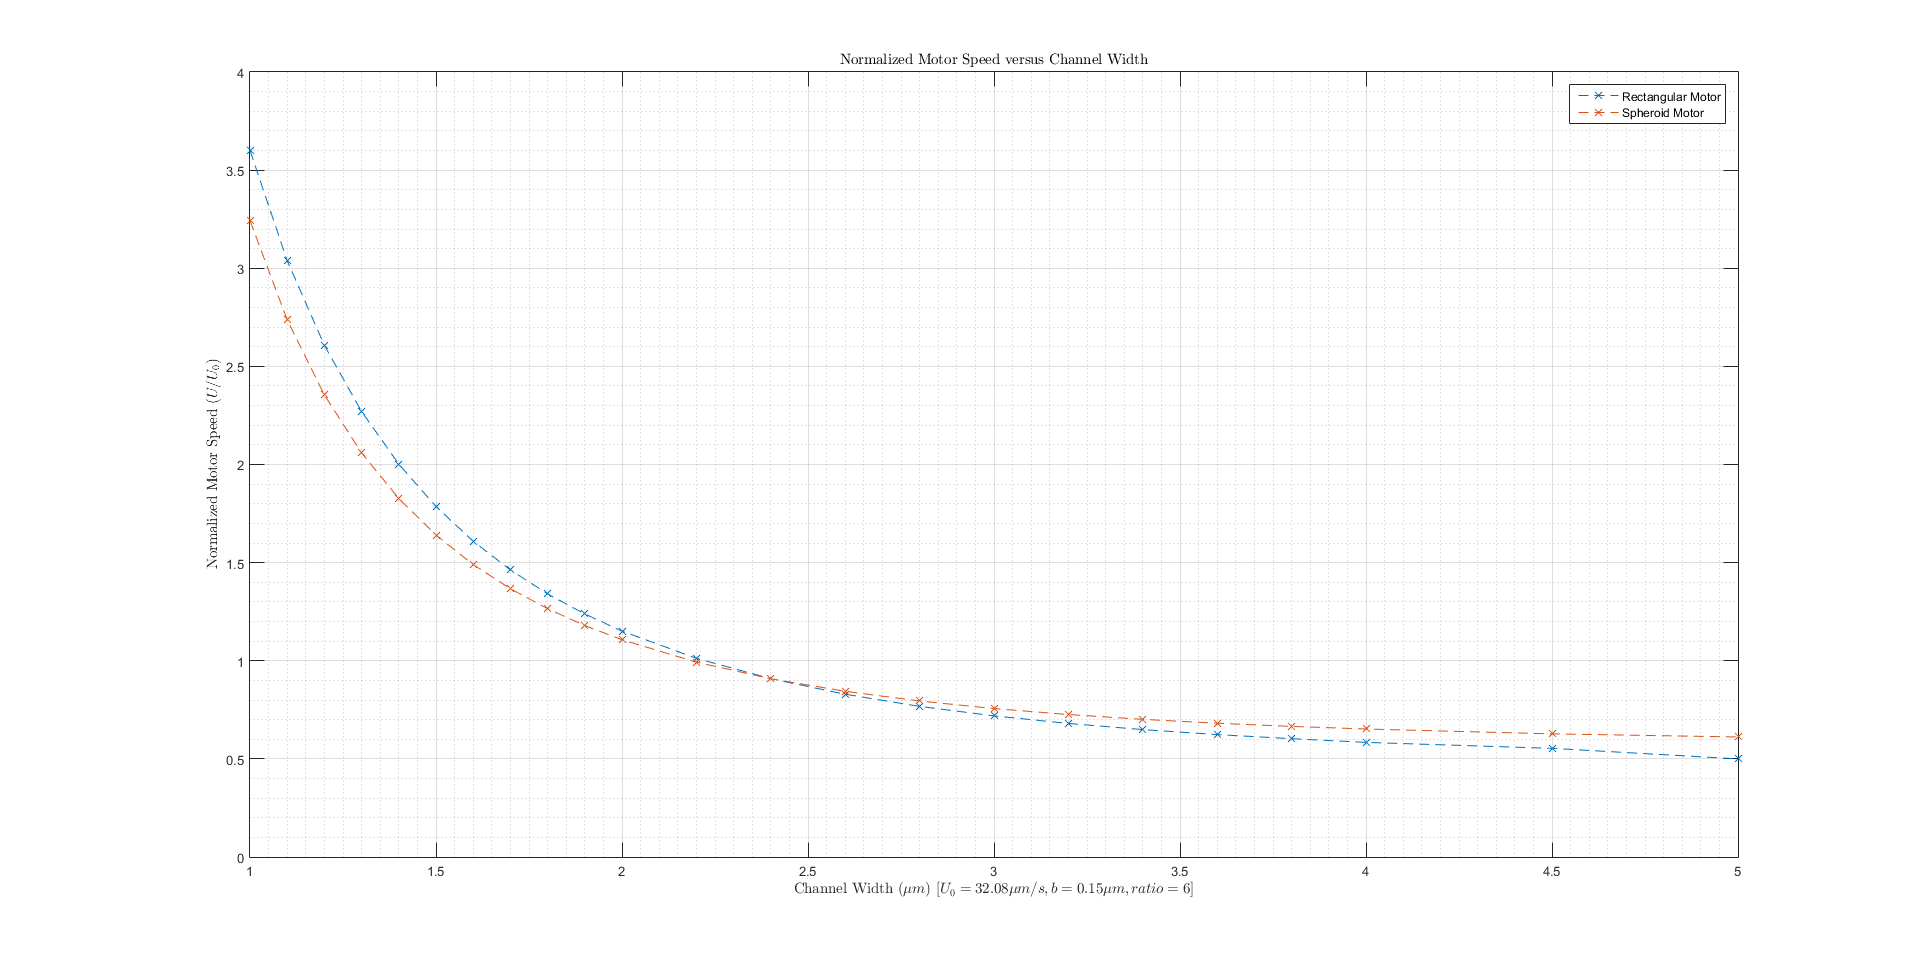
\includegraphics[width=\linewidth, height=3.5in]{2016-12-18-InfluenceOfMotorShape.png}
\caption{Comparison Between Spheroid Motor and Rectangular Motor}\label{2016-12-18-CBSMARM}
\end{figure}
\end{enumerate}

\labday{Friday, 23 December 2016}
When I begin to benchmark source/sink motor, there are several problems worth noting.
\begin{enumerate}
\item
The analytic results given in paper\cite{Nourhani2016} are derived under the constrain of zero net flux. I previous assigned a constant flux on the motor surface cannot satisfy this condition.
\item
In order to construct a boundary condition which satisfies the zero net flux condition, I still use tanh function to specify a continuous boundary condition. However, I add an additional transformation to meet the zero net flux condition:
\begin{equation}
\{[-1,1]+a\}\times b=[-1,k]
\end{equation}
where
\begin{equation}
a=\frac{-1+k}{1+k}\\
b=\frac{1+k}{2}
\end{equation}
$k$ is the area ratio between negative charged surface and positive charged surface.
\item
the sqrt function in COMSOL is strange. I met error message which shows that sqrt cannot do calculation with a negative number. However, I still want sqrt function valid for negative numbers. Finally, I found if I allow complex output in solve setting. This error could be solved.
\end{enumerate}
\labday{Sunday, 25 December 2016}
I finally finished calculation of previous listed plan. However, more questions emerged during my calculation process. I am very confused currently. I will record some of these questions here:
\begin{enumerate}
\item
When $\eta_0=0$, theoretical calculations show that Source/Sink motor speed is exactly two times of Source/Inert Motor. Mathematically speaking, there is because the absolute whole flux of Source/Sink motor is two times of Source/Inert Motor. What's the physical explanation of this?
\item
A strange convergence of Source/Sink motor with large aspect ratio under channel confinement. It's behavior is very different from Source/Inert motor. I still don't know why. ref: Fig. \ref{2016-12-25-SSMSCUFCW} and Fig. \ref{2016-12-18-SIMSCUFCW}.
\item
When $\eta_0=0$, Source/Sink motor speed is still exactly two times of Source/Inert Motor, as two curves shown in Fig. \ref{2016-12-25-SSMSCUDCW} and Fig. \ref{2016-12-25-SIMSCUDCW} collapsed into one curve. It seems that the both Source/Sink motor and Source/Inert motor speed up equally under channel confinement.
\item Another interesting property is shown by Fig. \ref{2016-12-25-SBSISS}. The theoretical speed of Source/Sink motor with $\eta_0=0.2$ and Source/Inert motor with $\eta_0=0$ are very similar, which causes similar speed up as shown in Fig.\ref{2016-12-25-SSMSCUDCC2} and Fig. \ref{2016-12-18-SIMSCUDCC}.
\begin{figure}
\centering
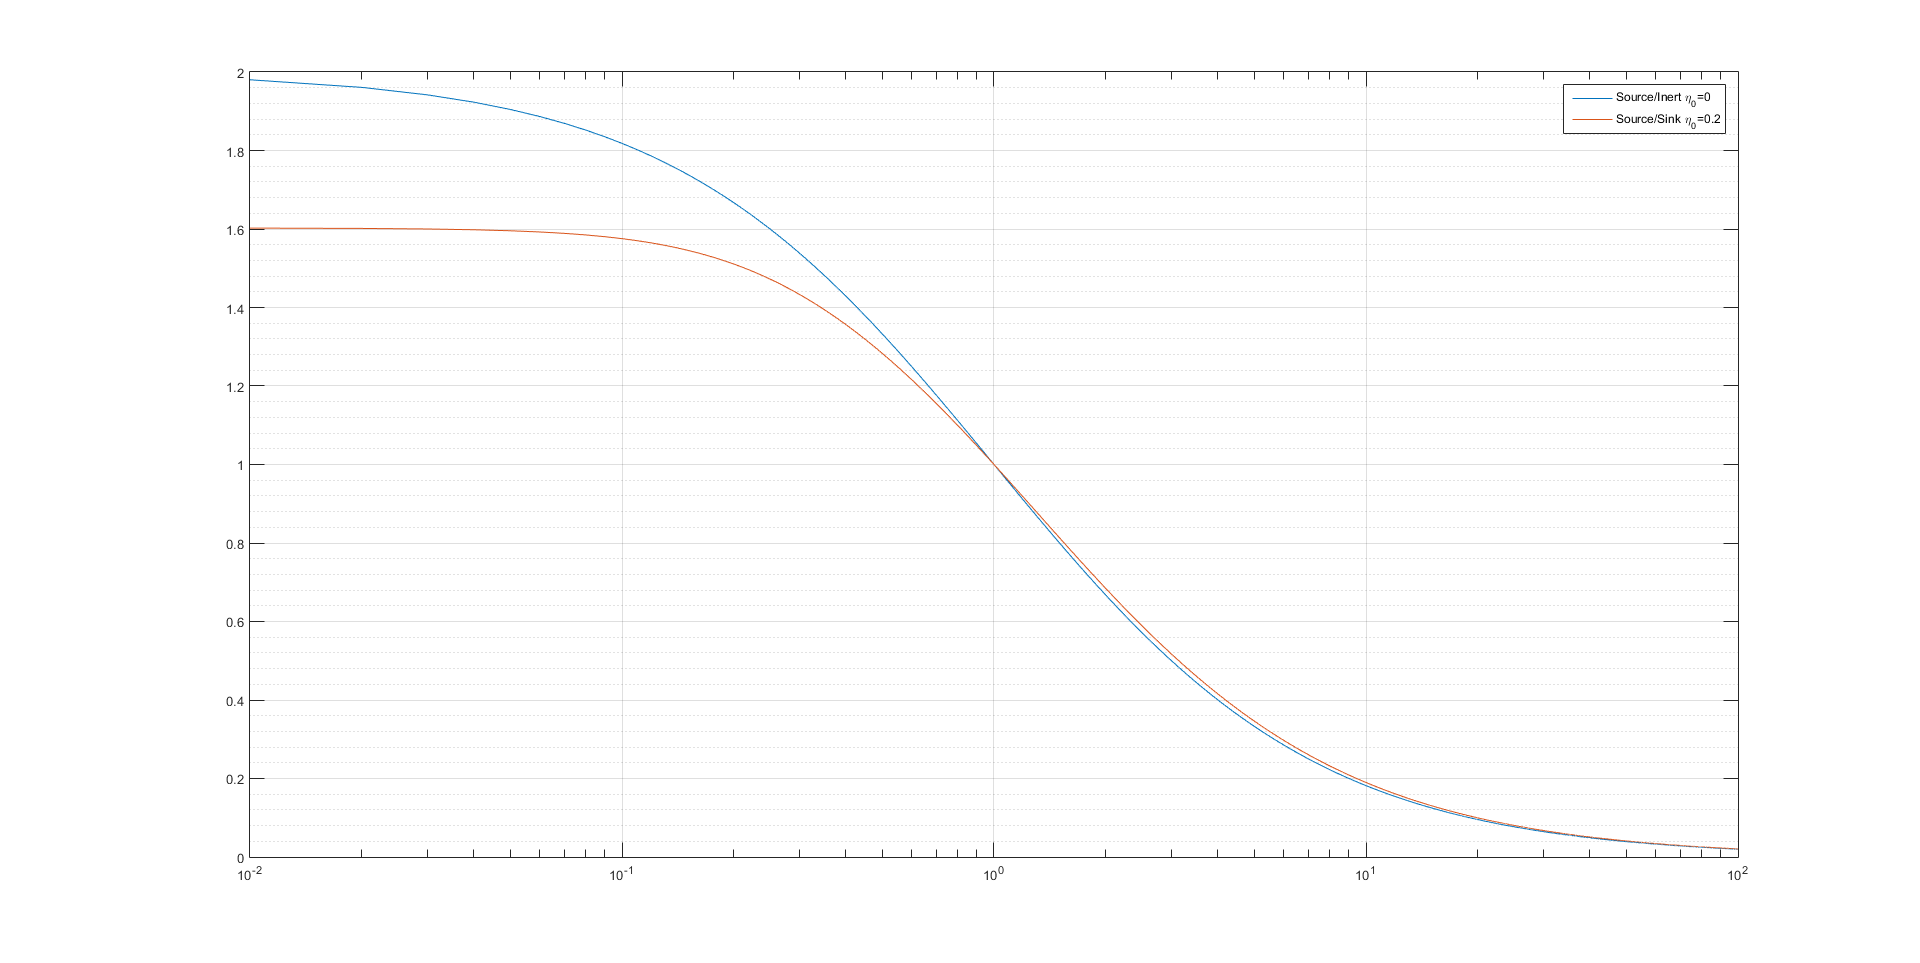
\includegraphics[width=\linewidth, height=3.5in]{2016-12-25-similar.png}
\caption{Similarity between Source/Inert motor ($\eta_0=0$) and Source/Sink motor ($\eta_0=0.2$)}\label{2016-12-25-SBSISS}
\end{figure}
\end{enumerate}
Many problems need to be answered. I will summerize my current finished calculation results tomorrow. Hope it could help me realize my current problem more clearly.
\labday{Monday, 20 February, 2017}
\experiment{Report 2 - Winter Vacation Progress From Jan. 17, 2017 to Feb. 17, 2017}
\section{Introduction}
Inspired by the work\cite{MozaffariSharifi-MoodKoplikEtAl2016}\cite{LeeLeal1980} which solved the motion of spherical active colloidal near solid wall analytically, I was wondering whether I could solve the motion of spheroidal active motor near solid wall. A key method applied in that paper is the author chose an uncommon coordinate system-bispherical coordinate system which naturally matches the geometry of spherical Janus particle confined by solid wall. Then I referred to \cite{MorseFeshbach1953} and \cite{MoonSpencer1988}, I first knew that there are many other orthogonal coordinate system. When I saw the prolate coordinate system, I knew that it was the one I am looking for to solve spheroidal active motor related problem, at least, in free space. To kill my boring time, I try to solve the motion of spheroid active motor in free space analytically. The solution of this problem could be generally divided into two parts: electrostatic part and hydrodynamic part. The electrostatic part needs to solve Laplace equation. Those who did field theory had solved the general solution of Laplace equation under prolate spheroidal coordinate long ago. All I need to do is to specify correct boundary condition. As for the hydrodynamic part, I need to solve creeping flow equation under prolate spheroidal coordinate. Fortunately, this problem could be solved by applying Stokes stream function\cite{HappelBrenner1983} because of the axis-symmetry of the system I want to solve. Then, I expect I could the motion of spheroidal active motor in free space. I will start from the electrostatic part.
\section{Electrostatic Part}
\subsection{Governing Equation}
\begin{equation}
\nabla^2\psi=0
\end{equation}
\subsection{Boundary Conditions}
\begin{enumerate}
\item
The electrical potential is assume as zero at infinity, i.e.
\begin{equation}
\psi|_{r\rightarrow\infty}=0
\end{equation}
\item
The normal component of electrical field along the motor surface is assume to be constant\cite{Kline2006}, i.e.
\begin{equation}
\nabla\psi \cdot \uv n = \frac{\sigma_0}{\epsilon}
\end{equation}
\end{enumerate}
\section{Prolate Spheroidal Coordinate}
This section is used for reviewing some useful properties about prolate spheroidal coordinate system.\cite{MoonSpencer1988}
\subsection{Coordinates Symbols}
\begin{equation}
\left\{
\begin{aligned}
u^1&=\xi , 0\le\xi<\infty\\
u^2&=\theta,0\le\theta\le\pi\\
u^3&=\phi,0\le\phi<2\pi
\end{aligned}
\right.
\end{equation}
\subsection{Transformation Relations}
\begin{equation}
\left\{
\begin{aligned}
x&=c\sinh\xi\sin\theta\cos\phi\\
y&=c\sinh\xi\sin\theta\sin\phi\\
z&=c\cosh\xi\cos\theta
\end{aligned}
\right.
\end{equation}
\subsection{Coordinate Surfaces}
\begin{equation}
\left\{
\begin{aligned}
\frac{x^2}{c^2\sinh^2\xi}+\frac{y^2}{c^2\sinh^2\xi}+\frac{z^2}{c^2\cosh^2\xi}&=1\\
\frac{x^2}{c^2\sin^2\theta}-\frac{y^2}{c^2\sin^2\theta}+\frac{z^2}{c^2\cos^2\theta}&=1\\
\tan\phi&=\frac{y}{x}
\end{aligned}
\right.
\end{equation}
\subsection{Metric Coefficients}
\begin{equation}
g_{11}=g_{22}=c^2(\sinh^2\xi+\sin^2\theta)\ \ g_{33}=c^2\sinh^2\xi\sin^2\theta
\end{equation}
\subsection{Differential Operators}
\subsubsection{Gradient Operator}
\begin{equation}
\nabla=\frac{1}{c(\sinh^2\xi+\sin^2\theta)^{\frac{1}{2}}}\left[\uv a_{\xi} \pd{}{\xi}+\uv a_{\theta}\pd{}{\theta}\right]+\frac{\uv a_{\phi}}{c\sinh\xi\sin\theta}\pd{}{\phi}
\end{equation}
\subsubsection{Laplace's Operator}
\begin{equation}
\nabla^2=\frac{1}{c^2(\sinh^2\xi+\sin^2\theta)}\left[\pdd{}{\xi}+\coth\xi\pd{}{\xi}+\pdd{}{\theta}+\cot\theta\pd{}{\theta}\right]+\frac{1}{c^2\sinh^2\xi\sin^2\theta}\pdd{}{\phi}
\end{equation}
\section{Separation of Laplace's Equation}
Consider axis-symmetrical case, i.e. $\psi$ is independent of $\phi$ and assume separation of variables:
\begin{equation}
\psi=\Xi(\xi)\Theta(\theta)
\end{equation}
Then, Laplace's Equation could be reduced as:
\begin{equation}
\left\{
\begin{aligned}
\dd{\Xi}{\xi}+\coth\xi\d{\Xi}{\xi}-n(n+1)\Xi&=0\\
\dd{\Theta}{\theta}+\cot\theta\d{\Theta}{\theta}+n(n+1)\Theta&=0
\end{aligned}
\right.
\end{equation}
The general solution of above ordinary differential equation is given by Legendre functions and the most general solution of Laplace's equation could be expressed as\cite{MoonSpencer1988}:
\begin{equation}
\begin{aligned}
\psi&=\sum_{n=0}^\infty \Xi_n(\xi)\Theta_n(\theta)\\
&=\sum_{n=0}^\infty \left[A_n \mathscr{P}_n(\cosh\xi)+B_n \mathscr{Q}_n(\cosh\xi)\right]\left[C_n\mathscr{P}_n(\cos\theta)+D_n\mathscr{Q}_n(\cos\theta)\right]
\end{aligned}
\end{equation}
where $\mathscr{P}_n$ is first kind of Legendre polynomial of nth order and $\mathscr{Q}_n$ is second kind of Legendre polynomial of nth order. Their explicit expressions are recorded below for reference:
\begin{equation}
\mathscr{P}_n(x)=\frac{1}{2^n}\sum_{k=0}^n
\begin{pmatrix}
n\\
k
\end{pmatrix}^2
(x-1)^{n-k}(x+1)^k
\end{equation}
\begin{equation}
\mathscr{Q}_n(x)=\frac{n!}{1\cdot3\cdots(2n+1)}\left[x^{-(n+1)}+\frac{(n+1)(n+2)}{2(2n+3)}x^{-(n+3)}+\frac{(n+1)(n+2)(n+3)(n+4)}{2\cdot4\cdot(2n+3)(2n+5)}x^{-(n+5)}+\cdots\right]
\end{equation}
\section{Boundary Conditions}
The next step is to match general solution to specific boundary conditions which are of interests.
\subsection{Physical Consideration}
$\mathscr{Q}_n(\cos\theta)$ becomes infinity at z-axis, i.e. $\theta=0, \pi$. Thus, $\mathscr(Q)_n(\cos\theta)$ term must vanish in the general solution. Then, the general solution could be simplified as:
\begin{equation}
\psi=\sum_{n=0}^\infty A_n \mathscr{P}_n(\cosh\xi)\mathscr{P}_n(\cos\theta)+B_n\mathscr{Q}_n(\cosh\xi)\mathscr{P}_n(\cos\theta)
\end{equation}
\subsection{Boundary Conditions at Infinity}
The electrical potential is set as zero at infinity, i.e.
\begin{equation}
\psi(\xi,\theta)|_{\xi\rightarrow\infty}=0
\end{equation}
Note that
\begin{equation}
\mathscr{P}_n(\cosh\xi)|_{\xi\rightarrow\infty}=\infty, n\ge1
\end{equation}
\begin{equation}
\mathscr{Q}_n(\cosh\xi)|_{\xi\rightarrow\infty}=0,n\ge0
\end{equation}
Therefore, the general solution could be further simplified as:
\begin{equation}
\psi=A_0+\sum_{n=0}^\infty B_n \mathscr{Q}_n(\cosh\xi)\mathscr{P}_n(\cos\theta)
\end{equation}
Because of the arbitrariness of electrical potential, the constant $A_0$ could be set directly as 0, then
\begin{equation}
\psi=\sum_{n=0}^\infty B_n \mathscr{Q}_n(\cosh\xi)\mathscr{P}_n(\cos\theta)
\end{equation}
\subsection{Boundary Conditions at Motor Surface}
The assumption of constant normal surface flux at motor flux results in constant normal component of electrical field at the outer edge of diffusion layer. Using Laplace equation to describe the electrostatic part is only valid beyond the diffusion layer. Therefore, the boundary conditions is given at the outer edge of diffusion layer and requires that
\begin{equation}
\nabla\psi \cdot \uv n= \frac{f(\xi,\theta)}{\epsilon},\xi=\xi_0
\end{equation}
where $\uv n$ is unit normal vector of motor surface and $f(\xi,\theta)$ is coverage function which is defined as
\begin{equation}
f(\xi,\theta)=
\begin{cases}
&\sigma_+,\theta<\theta_0\\
&\sigma_-,\theta>\theta_0
\end{cases}
\end{equation}
$\sigma_+$ and $\sigma_-$ describe equivalent surface charge at active surface and inert surface respectively.\\
Note that the nabla operator in the prolate spheroidal coordinate is
\begin{equation}
\nabla=\frac{1}{c(\sinh^2\xi+\sin^2\theta)^{\frac{1}{2}}}\left[\uv a_{\xi} \pd{}{\xi}+\uv a_{\theta}\pd{}{\theta}\right]+\frac{\uv a_{\phi}}{c\sinh\xi\sin\theta}\pd{}{\phi}
\end{equation}
Then,
\begin{equation}
\pd{\psi}{\xi}=\sinh\xi\sum_{n=0}^\infty B_n \mathscr{Q}_n^\prime(\cosh\xi)\mathscr{P}_n(\cos\theta)
\end{equation}
\begin{equation}
\pd{\psi}{\theta}=-\sin\theta\sum_{n=0}^\infty B_n\mathscr{Q}_n(\cosh\xi)\mathscr{P}_n^\prime(\cos\theta)
\end{equation}
\begin{equation}
\pd{\psi}{\phi}=0
\end{equation}
Therefore,
\begin{equation}
\v{E}=E_\xi \uv{a}_\xi+E_\theta\uv{a}_\theta
\end{equation}
where
\begin{equation}
E_\xi=\frac{1}{c(\sinh^2\xi+\sin^2\theta)^{\frac{1}{2}}}\sinh\xi\sum_{n=0}^\infty B_n \mathscr{Q}_n^\prime(\cosh\xi)\mathscr{P}_n(\cos\theta)
\end{equation}
\begin{equation}
E_\theta=-\frac{1}{c(\sinh^2\xi+\sin^2\theta)^{\frac{1}{2}}}\sin\theta\sum_{n=0}^\infty B_n\mathscr{Q}_n(\cosh\xi)\mathscr{P}_n^\prime(\cos\theta)
\end{equation}
The constant $B_n$ is determined by boundary condition at motor surface, i.e.
\begin{equation}
E_\xi(\xi_0,\theta)=\frac{1}{c(\sinh^2\xi_0+\sin^2\theta)^{\frac{1}{2}}}\sinh\xi_0\sum_{n=0}^\infty B_n \mathscr{Q}_n^\prime(\cosh\xi_0)\mathscr{P}_n(\cos\theta)=\frac{f(\xi_0,\theta)}{\epsilon}
\end{equation}
Note the orthogonality of Legendre polynomials:
\begin{equation}
\int_{-1}^{1}P_m(x)P_n(x)\mathrm{d}x=\frac{2}{2n+1}\delta_{mn}
\end{equation}
Thus,
\begin{equation}
\begin{aligned}
\sum_{n=0}^\infty B_n \mathscr{Q}^\prime_{n}(\cosh\xi_0)\int_{-1}^1\mathscr{P}_n(\cos\theta)\mathscr{P}_m(\cos\theta)\mathrm{d}\cos\theta&=\int_{-1}^1\frac{f(\xi_0,\theta)}{\epsilon}\frac{c(\sinh^2\xi_0+\sin^2\theta)^{\frac{1}{2}}}{\sinh\xi_0}\mathscr{P}_m(\cos\theta)\mathrm{d}\cos\theta\\
B_m\mathscr{Q}_m^\prime(\cosh\xi_0)\frac{2}{2m+1}&=\frac{c}{\epsilon\sinh\xi_0}\int_{-1}^1f(\xi_0,\theta)(\sinh^2\xi_0+\sin^2\theta)^{\frac{1}{2}}\mathscr{P}_m(\cos\theta)\mathrm{d}\cos\theta
\end{aligned}
\end{equation}
\begin{equation}
B_m=\frac{2m+1}{2}\frac{1}{\mathscr{Q}_m^\prime(\cosh\xi_0)}\frac{c}{\epsilon\sinh\xi_0}\int_{-1}^1f(\xi_0,\theta)(\sinh^2\xi_0+\sin^2\theta)^{\frac{1}{2}}\mathscr{P}_m(\cos\theta)\mathrm{d}\cos\theta
\end{equation}
\section{Summary of Electrostatic Part}
Now, electrostatic part has been fully solved. Relevant results are listed below for later usage.
\subsection{Electrical Potential}
\begin{equation}
\psi=\sum_{n=0}^\infty B_n \mathscr{Q}_n(\cosh\xi)\mathscr{P}_n(\cos\theta)
\end{equation}
where
\begin{equation}
B_n=\frac{2n+1}{2}\frac{1}{\mathscr{Q}_n^\prime(\cosh\xi_0)}\frac{c}{\epsilon\sinh\xi_0}\int_{-1}^1f(\xi_0,\theta)(\sinh^2\xi_0+\sin^2\theta)^{\frac{1}{2}}\mathscr{P}_n(\cos\theta)\mathrm{d}\cos\theta
\end{equation}
Consider the dimension of motor, 
\begin{equation}
c=\sqrt{a^2-b^2}
\end{equation}
\begin{equation}
\cosh\xi_0=\frac{a}{c}=\left[1-\left(\frac{b}{a}\right)^2\right]^{-\frac{1}{2}}
\end{equation}
\subsection{Electrical Field}
\begin{equation}
\v{E}=E_\xi \uv{a}_\xi+E_\theta\uv{a}_\theta
\end{equation}
where
\begin{equation}\label{Sln_E_xi}
E_\xi=\frac{1}{c(\sinh^2\xi+\sin^2\theta)^{\frac{1}{2}}}\sinh\xi\sum_{n=0}^\infty B_n \mathscr{Q}_n^\prime(\cosh\xi)\mathscr{P}_n(\cos\theta)
\end{equation}
\begin{equation}\label{Sln_E_theta}
E_\theta=-\frac{1}{c(\sinh^2\xi+\sin^2\theta)^{\frac{1}{2}}}\sin\theta\sum_{n=0}^\infty B_n\mathscr{Q}_n(\cosh\xi)\mathscr{P}_n^\prime(\cos\theta)
\end{equation}
$E_\theta$ component, which induces the electroosmosis flow around motor surface, is essential for the coupling between electrostatic part and hydrodynamic part.
\section{Hydrodynamic Part}
This section will address the problem which is relevant to hydrodynamic aspect. Because of the feature of system I am interested, the Reynold number is assume to be very small. Thus, the creeping flow equation is assume valid. I will only consider the axis-symmetrical case in 3D. Then, it's useful to introduce the concept of stream function.\cite{HappelBrenner1983} In the following contents, I will describe these aspects in detail.
\subsection{Governing Equation}
\begin{equation}
\left\{
\begin{aligned}
\mu\nabla^2\v v&=\grad P\\
\div \v v&=0
\end{aligned}
\right.
\end{equation}
\subsection{Boundary Condition}
\begin{enumerate}
\item
The fluid is assume at rest at infinity, i.e.
\begin{equation}
\v v|_{r\rightarrow\infty}=0
\end{equation}
\item
The slippery velocity at motor surface is assumed to be proportional to tangential component of electrical field, i.e.
\begin{equation}
\v v_s=\mu_{motor}\v E_t
\end{equation}
where $\mu_{motor}$ is the mobility of motor surface and $\v E_t$ is the tangential component of electrical field.\\
Therefore, the boundary condition at motor surface is written as:
\begin{equation}
\v v=v_s+U_{motor}=\mu_{motor}\v E_t+U_{motor}
\end{equation}
where $U_{motor}$ is the self-phoresis speed of motor.
\end{enumerate}
\section{Stream Function}
The interested system is assumed to be axis-symmetrical, which combined with the impressible condition, will guarantee the existence of stream function $\varphi$. The stream function is defined as:
\begin{equation}
\varphi=\frac{Q}{2\pi}=\frac{1}{2\pi}\int_{S}\v v\cdot\uv n\mathrm{d}S=\frac{1}{2\pi}\int_{s_0}^s\int_{0}^{2\pi}\v v\cdot \uv n \tilde{\omega}\mathrm{d}\phi\mathrm{d}s
\end{equation}
where $Q$ is the flux of prescribed surface $S$, $s$ is the arc length of meridian and $\tilde{\omega}$ is the radial length of meridian.
\subsection{Relations between stream function and local velocity}
Also note that
\begin{equation}
\varphi=\int_{s_0}^s\mathrm{d}\varphi=\int_{s_0}^s\v t\cdot \grad \varphi \mathrm{d}s
\end{equation}
where $\v t$ is the tangential vector of meridian. Thus,
\begin{equation}
\varphi=\int_{s_0}^s\v t\cdot \grad \varphi \mathrm{d}s=\int_{s_0}^s\v v\cdot \uv n\tilde{\omega}\mathrm{d}s
\end{equation}
It gives that
\begin{equation}
\v v \cdot \uv n\tilde{\omega}=\v t \cdot \grad \varphi
\end{equation}
i.e.
\begin{equation}
\v v=\frac{1}{\tilde{\omega}}\uv{i}_{\phi}\times\grad\varphi
\end{equation}
Project velocity $\v v$ in axis-symmetrical orthogonal coordinates system $\{q_1,q_2,\phi\}$:
\begin{equation}\label{eqn_velocity}
\left\{
\begin{aligned}
v_1&=-\frac{h_2}{\tilde{\omega}}\pd{\varphi}{q_2}\\
v_2&=\frac{h_1}{\tilde{\omega}}\pd{\varphi}{q_1}
\end{aligned}
\right.
\end{equation}
\subsection{Dynamical equations satisfied by stream function}
In this section, I will expression the common creeping flow equation in terms of stream function $\varphi$. In order to achieve that, let's first consider the curl of velocity field in a orthogonal coordinate system $\{q_1,q_2,\phi\}$, i.e.
\begin{equation}
\begin{aligned}
\gv \omega=\curl{\v  v}&=h_1h_2h_3
\begin{pmatrix}
\frac{\uv i_1}{h_1}&\frac{\uv i_2}{h_2}&\frac{\uv i_3}{h_3}\\
\pd{}{q_1}&\pd{}{q_2}&\pd{}{q_3}\\
\frac{v_1}{h_1}&\frac{v_2}{h_2}&\frac{v_3}{h_3}
\end{pmatrix}\\
&=\uv i_\phi h_1h_2\left[\pd{}{q_1}\left(\frac{v_2}{h_2}\right)-\pd{}{q_2}\left(\frac{v_1}{h_1}\right)\right]
\end{aligned}
\end{equation}
Express above result in terms of stream function, we have
\begin{equation}
\gv \omega=\frac{\uv i_\phi}{\tilde\omega}E^2\varphi
\end{equation}
where
\begin{equation}\label{operatorE2}
E^2=\tilde{\omega}h_1h_2\left[\pd{}{q_1}\left(\frac{1}{\tilde{\omega}}\frac{h_1}{h_2}\pd{}{q_1}\right)+\pd{}{q_2}\left(\frac{1}{\tilde{\omega}}\frac{h_2}{h_1}\pd{}{q_2}\right)\right]
\end{equation}
Note that Naiver-Stokes equation is
\begin{equation}
\rho(\pd{\v v}{t}+\v v\cdot\grad\v v)-\mu\nabla^2\v v=-\grad P
\end{equation}
Express Naiver-Stokes equation by $\gv \omega$, we have
\begin{equation}
\pd{\gv \omega}{t}-\curl{\v v\times \gv \omega}+\nu\curl{\curl{\gv \omega}}=0
\end{equation}
where $\nu=\frac{\mu}{\rho}$ is the kinematic viscosity.\\
Re-express by stream function, we obtain that
\begin{equation}
\nu E^4\varphi -\tilde{\omega}\left(\pd{\varphi}{z}\pd{}{\tilde{\omega}}-\pd{\varphi}{\tilde{\omega}}\pd{}{z}\right)\frac{E^2\varphi}{\tilde{\omega}^2}-\pd{}{t}(E^2\varphi)=0
\end{equation}
For the low Reynold number case, we could ignore inertial effect. Then, above equation could be reduced as
\begin{equation}
E^4\varphi-\frac{1}{\nu}\pd{}{t}\left(E^2\varphi\right)=0
\end{equation}
For the steady case, above equation could further reduced as
\begin{equation}
E^4\varphi=0
\end{equation}
\section{Separation in prolate spheroidal coordinate}
Because of the geometry of the interested system, prolate spheroidal coordinate system is more convenient for problem solving. We first express operator $E^2$ in prolate spheroidal coordinate system. Note that in prolate spheroidal coordinate system,
\begin{equation}
\left\{
\begin{aligned}
x&=c\sinh\xi\sin\theta\cos\phi\\
y&=c\sinh\xi\sin\theta\sin\phi\\
z&=c\cosh\xi\cos\theta
\end{aligned}
\right.
\end{equation}
\begin{equation}
h_\xi^2=h_\theta^2=\frac{1}{c^2\left(\sinh^2\xi+\sin^2\theta\right)} \ \ \ \ h_\phi^2=\frac{1}{c^2\sinh^2\xi\sin^2\theta}
\end{equation}
For convenience, denote that
\begin{equation}
\lambda =\cosh \xi \ \ \ \ \ \kappa=\cos\theta
\end{equation}
Then, note that
\begin{equation}\label{eqn_differential}
\left\{
\begin{aligned}
\pd{}{\xi}&=\sqrt{\lambda^2-1}\pd{}{\lambda}\\
\pd{}{\theta}&=\sqrt{1-\kappa^2}\pd{}{\kappa}\\
\end{aligned}
\right.
\end{equation}
and
\begin{equation}
\left\{
\begin{aligned}
\tilde{\omega}&=\sqrt{x^2+y^2}=c\sinh\xi\sin\theta=c\sqrt{\lambda^2-1}\sqrt{1-\kappa^2}\\
z&=c\lambda\kappa
\end{aligned}
\right.
\end{equation}
According to \ref{operatorE2}, the operator $E^2$ could be rewritten as
\begin{equation}
E^2=\frac{1}{c^2(\lambda^2-\kappa^2)}\left[\left(\lambda^2-1\right)\pdd{}{\lambda}+\left(1-\kappa^2\right)\pdd{}{\kappa}\right]
\end{equation}
\section{Trial Solution}
In order to obtain the solution of $E^4\varphi=0$, consider the trial solution which assumes that
\begin{equation}
\varphi=(1-\kappa^2)g(\lambda)
\end{equation}
Thus,
\begin{equation}
\begin{aligned}
E^2\varphi&=\frac{1}{c^2(\lambda^2-\kappa^2)}\left[\left(\lambda^2-1\right)\pdd{}{\lambda}+\left(1-\kappa^2\right)\pdd{}{\kappa}\right](1-\kappa^2)g(\lambda)\\
&=\frac{1}{c^2(\lambda^2-\kappa^2)}\left[(\lambda^2-1)(1-\kappa^2)g^{\prime\prime}-2g(1-\kappa^2)\right]\\
&=\frac{(1-\kappa^2)}{c^2(\lambda^2-\kappa^2)}G(\lambda)
\end{aligned}
\end{equation}
where
\begin{equation}
G(\lambda)=(\lambda^2-1)g^{\prime\prime}(\lambda)-2g(\lambda)
\end{equation}
Repeat above process and after a lengthy calculation, we obtain that
\begin{equation}
\begin{aligned}
E^4\varphi&=E^2\left[\frac{(1-\kappa^2)}{c^2(\lambda^2-\kappa^2)}G(\lambda)\right]\\
&=\frac{(\kappa^2-1)(\lambda^2-1)\left[4(G-\lambda G^\prime)+(\lambda^2-\kappa^2)G^{\prime\prime}\right]}{c^4(\kappa^2-\lambda^2)^3}
\end{aligned}
\end{equation}
In order to satisfy equation $E^4\varphi=0$, following two equations must be satisfied simultaneously:
\begin{equation}
\left\{
\begin{aligned}
G-\lambda G^\prime&=0\\
G^{\prime\prime}&=0
\end{aligned}
\right.
\end{equation}
It's easy to find the above equations has only solution:
\begin{equation}\label{eqn-lambdapart}
G=C_1\lambda=(\lambda^2-1)g^{\prime\prime}-2g
\end{equation}
Note that this ordinary differential equation has a particular solution which is
\begin{equation}
g_{p}=-\frac{1}{2}C_1\lambda
\end{equation}
i.e.
\begin{equation}
(\lambda^2-1)g^{\prime\prime}_{p}-2g_p=C_1\lambda
\end{equation}
Then, we need to solve following homogeneous equation to obtain general solution,
\begin{equation}
(\lambda^2-1)g_h^{\prime\prime}-2g_{h}=0
\end{equation}
Note that
\begin{equation}
\d{}{\lambda}\left[(\lambda^2-1)g_h^\prime-2g_h\lambda\right]=0
\end{equation}
Thus,
\begin{equation}
(\lambda^2-1)g_h^\prime-2g_h\lambda=C_2
\end{equation}
Also note that
\begin{equation}
\d{}{\lambda}\left[\frac{g_h}{\lambda^2-1}\right]=\frac{C_2}{(\lambda^2-1)^2}
\end{equation}
Therefore, the solution of homogeneous part is
\begin{equation}
\begin{aligned}
g_h&=C_2(\lambda^2-1)\int\frac{\mathrm{d}\lambda}{(\lambda^2-1)^2}+C_3(\lambda^2-1)\\
&=
\begin{cases}
\frac{C_2}{2}\left[\mathrm{arctanh}(\lambda)(\lambda^2-1)-\lambda\right]+C_3(\lambda^2-1),&0\le\lambda<1\\
\frac{C_2}{2}\left[\mathrm{arccoth}(\lambda)(\lambda^2-1)-\lambda\right]+C_3(\lambda^2-1),&\lambda>1
\end{cases}
\end{aligned}
\end{equation}
Then, the general solution of \ref{eqn-lambdapart} could be written as
\begin{equation}
g(\lambda)=g_p(\lambda)+g_h(\lambda)=
\begin{cases}
-\frac{1}{2}C_1\lambda+\frac{C_2}{2}\left[\mathrm{arctanh}(\lambda)(\lambda^2-1)-\lambda\right]+C_3(\lambda^2-1),&0\le\lambda<1\\
-\frac{1}{2}C_1\lambda+\frac{C_2}{2}\left[\mathrm{arccoth}(\lambda)(\lambda^2-1)-\lambda\right]+C_3(\lambda^2-1),&\lambda>1
\end{cases}
\end{equation}
Finally, the general form of stream function which satisfied $E^4\varphi=0$ in prolate spheroidal coordinate is:
\begin{equation}
\varphi=
\begin{cases}
(1-\kappa^2)\left\{-\frac{1}{2}C_1\lambda+\frac{C_2}{2}\left[\mathrm{arctanh}(\lambda)(\lambda^2-1)-\lambda\right]+C_3(\lambda^2-1)\right\},&0\le\lambda<1\\
(1-\kappa^2)\left\{-\frac{1}{2}C_1\lambda+\frac{C_2}{2}\left[\mathrm{arccoth}(\lambda)(\lambda^2-1)-\lambda\right]+C_3(\lambda^2-1)\right\},&\lambda>1
\end{cases}
\end{equation}
\section{Boundary Conditions}
In this section, I will firstly express relevant boundary conditions in terms of stream function. Then I will match boundary conditions with the general form of prolate spheroidal coordinate derived in last section to determine unknown constants. For convenience, all  relevant boundary conditions are rewritten by choosing motor as reference frame.
\subsection{Boundary Condition at Infinity}
By choosing motor itself as reference frame, original rest fluid at infinity becomes fluid with uniform motor speed. Thus, boundary condition at infinity becomes
\begin{equation}
\varphi|_{\lambda\rightarrow\infty}=\frac{1}{2}U_{motor}\tilde{\omega}^2=\frac{1}{2}U_{motor}c^2(\lambda^2-1)(1-\kappa^2)
\end{equation}
\subsection{Boundary Conditions at Motor Surface}
Original normal direction at motor surface is assumed to be no slippery condition and tangential direction has slippery velocity which is assume to be proportional to the tangential component of electrical field. Choosing motor as reference frame, these conditions could be rewritten as
\begin{enumerate}
\item
Normal component of fluid velocity field at motor surface is zero, then
\begin{equation}
v_{\xi}=-\frac{h_\theta}{\tilde{\omega}}\pd{\varphi}{\theta}=\frac{1}{c\sqrt{\lambda^2-\kappa^2}}c\sqrt{\lambda^2-1}\sqrt{1-\kappa^2}\sqrt{1-\kappa^2}\pd{\varphi}{\kappa}=\frac{(1-\kappa^2)\sqrt{\lambda^2-1}}{\sqrt{\lambda^2-\kappa^2}}\pd{\varphi}{\kappa}=0
\end{equation}
i.e.
\begin{equation}
\varphi(\lambda_0,\kappa)=0
\end{equation}
where motor surface is characterized by surface $\lambda=\lambda_0$ and $\varphi=0$ at axis of symmetry has been taken into consideration.
\item Tangential component of fluid of velocity should be equal to the electroosmosis velocity caused by electrical field, then
\begin{equation}
v_\theta=\frac{h_\xi}{\tilde{\omega}}\pd{\varphi}{\xi}=\frac{1}{c\sqrt{\lambda^2-\kappa^2}}c\sqrt{\lambda^2-1}\sqrt{1-\kappa^2}\sqrt{\lambda^2-1}\pd{\varphi}{\lambda}=\frac{(\lambda^2-1)\sqrt{1-\kappa^2}}{\sqrt{\lambda^2-\kappa^2}}\pd{\varphi}{\lambda}=\mu_{motor}E_\theta
\end{equation}
\end{enumerate}
i.e.
\begin{equation}
\frac{(\lambda^2-1)\sqrt{1-\kappa^2}}{\sqrt{\lambda^2-\kappa^2}}\pd{\varphi}{\lambda}=\mu_{motor}E_\theta
\end{equation}
Note that the tangential component of electrical field could be given independently by \ref{Sln_E_theta}.
\subsection{Matching with Boundary Conditions}
Note the geometry of motor that
\begin{equation}
\lambda_0=\cosh\xi_0=\frac{a}{c}=\left[1-\left(\frac{b}{a}\right)^2\right]^{-\frac{1}{2}}>1
\end{equation}
Then, the general form of stream function is
\begin{equation}\label{eqn_streamFunc}
\varphi{} = \left({\kappa{}}^2 - 1\right)\, \left(\frac{\lambda{}\, C_{1}}{2} - C_{3}\, \left({\lambda{}}^2 - 1\right) + \frac{C_{2}\, \left(\lambda{} - \mathop{\mathrm{arccoth}}\nolimits\!\left(\lambda{}\right)\, \left({\lambda{}}^2 - 1\right)\right)}{2}\right)
\end{equation}
First, consider the boundary condition at infinity and obviously,
\begin{equation}
C_3=\frac{1}{2}U_{motor}c^2
\end{equation}
To obtain above conclusion, we must assume $C_1$ and $C_2$ have opposite sign which is satisfied automatically in following derivation.\\
Then, consider the boundary conditions at motor surface and note that
\begin{equation}
\pd{\varphi}{\lambda}=- \left({\kappa{}}^2 - 1\right)\, \left(\frac{C_{2}\, \left(2\, \lambda{}\, \mathop{\mathrm{arccoth}}\nolimits\!\left(\lambda{}\right) - 2\right)}{2} - \frac{C_{1}}{2} + 2\, \lambda{}\, C_{3}\right)
\end{equation}
Thus, other two constants $C_1$ and $C_2$ are determined by following linear system,
\begin{equation}
\left\{
\begin{aligned}
(1-\kappa^2)\left\{-\frac{C_1\lambda_0}{2}+\frac{C_2}{2}\left[\mathrm{arccoth}(\lambda_0)(\lambda_0^2-1)-\lambda_0\right]+C_3(\lambda_0^2-1)\right\}&=0\\
-\frac{(\lambda_0^2-1)\sqrt{1-\kappa^2}}{\sqrt{\lambda_0^2-\kappa^2}} \left({\kappa{}}^2 - 1\right)\, \left(\frac{C_{2}\, \left(2\, \lambda_0{}\, \mathop{\mathrm{arccoth}}\nolimits\!\left(\lambda_0{}\right) - 2\right)}{2} - \frac{C_{1}}{2} + 2\, \lambda_0{}\, C_{3}\right)&=\mu_{motor}E_\theta
\end{aligned}
\right.
\end{equation}
The result is given below:
\begin{equation}
\left\{
\begin{aligned}
C_1&=\frac{4C_3}{\sigma_1}+\frac{\mu_{motor}E_\theta}{\sigma_3}\frac{\sigma_2}{\sigma_1}\\
C_2&=-\frac{2C_3(\lambda_0^2+1)}{\sigma_1}+\frac{\mu_{motor}E_\theta}{\sigma_3}\frac{2\lambda_0}{\sigma_1}
\end{aligned}
\right.
\end{equation}
where
\begin{equation}
\left\{
\begin{aligned}
\sigma_1&=-\lambda_0+\lambda_0^2\mathrm{arccoth}(\lambda_0)+\mathrm{arccoth}(\lambda_0)\\
\sigma_2&=-\lambda_0+\lambda_0^2\mathrm{arccoth}(\lambda_0)-\mathrm{arccoth}(\lambda_0)\\
\sigma_3&=\frac{(\lambda_0^2-1)(1-\kappa^2)^{3/2}}{\sqrt{\lambda_0^2-\kappa^2}}
\end{aligned}
\right.
\end{equation}
Substitute $C_1$, $C_2$ and $C_3$ back into \ref{eqn_streamFunc}:
\begin{equation}
\varphi=\varphi_{H}+\varphi_{E}
\end{equation}
where
\begin{equation}
\varphi_{H}=
\frac{1}{2}U_{motor}\tilde{\omega}^2\left\{1-\left[\frac{\frac{\lambda}{\lambda^2-1}-\frac{\lambda_0^2+1}{\lambda_0^2-1}\mathrm{arccoth}(\lambda)}{\frac{\lambda_0}{\lambda_0^2-1}-\frac{\lambda_0^2+1}{\lambda_0^2-1}\mathrm{arccoth}(\lambda_0)}\right]\right\}
\end{equation}
Note that
\begin{equation}
\tilde{\omega}=c\sqrt{\lambda^2-1}\sqrt{1-\kappa^2}
\end{equation}
\begin{equation}
\begin{aligned}
\varphi_{E}&=\frac{1}{2}(\kappa^2-1)\frac{\mu_{motor}E_\theta}{\sigma_3}\frac{\sigma_2}{\sigma_1}(\lambda-2\lambda_0)\\
&=-\frac{1}{2}\frac{\sqrt{\lambda_0^2-\kappa^2}}{(\lambda_0^2-1)\sqrt{1-\kappa^2}}\frac{\sigma_2}{\sigma_1}(\lambda-2\lambda_0)\mu_{motor}E_\theta
\end{aligned}
\end{equation}
Put these results together, the stream function could be written as
\begin{equation}
\varphi=\frac{1}{2}U_{motor}\tilde{\omega}^2\left\{1-\left[\frac{\frac{\lambda}{\lambda^2-1}-\frac{\lambda_0^2+1}{\lambda_0^2-1}\mathrm{arccoth}(\lambda)}{\frac{\lambda_0}{\lambda_0^2-1}-\frac{\lambda_0^2+1}{\lambda_0^2-1}\mathrm{arccoth}(\lambda_0)}\right]\right\}-\frac{1}{2}\frac{\sqrt{\lambda_0^2-\kappa^2}}{(\lambda_0^2-1)\sqrt{1-\kappa^2}}\frac{\sigma_2}{\sigma_1}(\lambda-2\lambda_0)\mu_{motor}E_\theta
\end{equation}
The first term is caused by the common hydrodynamic effect while the second term is the electrostatic effect caused by motor surface reaction which is coupled with the hydrodynamic motion as stream function clearly displayed.\\
Finally, note that above stream function is written by choosing motor body as reference frame. It could be easily transformed to laboratory frame by subtracting a uniform background with velocity $U_{motor}$, i.e.
\begin{equation}\label{eqn-streamfunc}
\begin{aligned}
\tilde\varphi&=\varphi-\frac{1}{2}U_{motor}\tilde{\omega}^2\\
&=-\frac{1}{2}U_{motor}\tilde{\omega}^2\left[\frac{\frac{\lambda}{\lambda^2-1}-\frac{\lambda_0^2+1}{\lambda_0^2-1}\mathrm{arccoth}(\lambda)}{\frac{\lambda_0}{\lambda_0^2-1}-\frac{\lambda_0^2+1}{\lambda_0^2-1}\mathrm{arccoth}(\lambda_0)}\right]-\frac{1}{2}\frac{\sqrt{\lambda_0^2-\kappa^2}}{(\lambda_0^2-1)\sqrt{1-\kappa^2}}\frac{\sigma_2}{\sigma_1}(\lambda-2\lambda_0)\mu_{motor}E_\theta(\lambda_0,\kappa), \lambda>1
\end{aligned}
\end{equation}
\section{Velocity Field, Fluid Stress, Resistance Force and Motor Speed}
As stream function of interested system has been explicitly calculated, all relevant quantities are ready for calculation. In this section, I will calculate the velocity field, fluid stress tensor, resistance force and finally to determined the self-phoresis speed of motor.
\subsection{Velocity Field}
According to \ref{eqn_velocity}, the velocity field and stream function have following relations:
\begin{equation}
\left\{
\begin{aligned}
v_{\xi}&=-\frac{h_\theta}{\tilde{\omega}}\pd{\varphi}{\theta}\\
v_{\theta}&=\frac{h_\xi}{\tilde\omega}\pd{\varphi}{\xi}
\end{aligned}
\right.
\end{equation}
Note differential relation given by ~\ref{eqn_differential}, velocity field could be calculated as following:
\begin{equation}
\left\{
\begin{aligned}
v_{\xi}&=-\frac{1}{c\sqrt{\lambda^2-1}\sqrt{1-\kappa^2}}\frac{1}{c\sqrt{\lambda^2-\kappa^2}}\left(-\sqrt{1-\kappa^2}\pd{\varphi}{\kappa}\right)=\frac{1}{c^2\sqrt{\lambda^2-1}\sqrt{\lambda^2-\kappa^2}}\pd{\varphi}{\kappa}\\
v_{\theta}&=\frac{1}{c\sqrt{\lambda^2-1}\sqrt{1-\kappa^2}}\frac{1}{c\sqrt{\lambda^2-\kappa^2}}\sqrt{\lambda^2-1}\pd{\varphi}{\lambda}=\frac{1}{c^2\sqrt{1-\kappa^2}\sqrt{\lambda^2-\kappa^2}}\pd{\varphi}{\lambda}
\end{aligned}
\right.
\end{equation}
Note that
\begin{equation}\label{eqn-1st}
\begin{aligned}
E_\theta(\lambda_0,\kappa)&=-\frac{1}{c(\sinh^2\xi+\sin^2\theta)^{\frac{1}{2}}}\sin\theta\sum_{n=0}^\infty B_n\mathscr{Q}_n(\cosh\xi)\mathscr{P}_n^\prime(\cos\theta)\\
&=-\frac{\sqrt{1-\kappa^2}}{c\sqrt{\lambda_0^2-\kappa^2}}\sum_{n=0}^\infty B_n\mathscr{Q}_n(\lambda_0)\mathscr{P}_n^\prime(\kappa)\\
\pd{\varphi_H}{\kappa}&=-\frac{1}{2}U_{motor}c^2(\lambda^2-1)(-2\kappa)\left[\frac{\frac{\lambda}{\lambda^2-1}-\frac{\lambda_0^2+1}{\lambda_0^2-1}\mathrm{arccoth}(\lambda)}{\frac{\lambda_0}{\lambda_0^2-1}-\frac{\lambda_0^2+1}{\lambda_0^2-1}\mathrm{arccoth}(\lambda_0)}\right]\\
\pd{\varphi_E}{\kappa}&=\frac{1}{2}\frac{1}{\lambda_0^2-1}\frac{\sigma_2}{\sigma_1}\frac{\mu_{motor}}{c}(\lambda-2\lambda_0)\sum_{n=0}^\infty B_n\mathscr{Q}_n(\lambda_0)\mathscr{P}_n^{\prime\prime}(\kappa)\\
\pd{\varphi_H}{\lambda}&=-\frac{1}{2}U_{motor}c^2(1-\kappa^2)\left\{\frac{1-\frac{\lambda_0^2+1}{\lambda_0^2-1}\left[2\lambda\mathrm{arccoth}(\lambda)-1\right]}{\frac{\lambda_0}{\lambda_0^2-1}-\frac{\lambda_0^2+1}{\lambda_0^2-1}\mathrm{arccoth}(\lambda_0)}\right\}\\
\pd{\varphi_E}{\lambda}&=\frac{1}{2}\frac{1}{\lambda_0^2-1}\frac{\sigma_2}{\sigma_1}\frac{\mu_{motor}}{c}\sum_{n=0}^\infty B_n \mathscr{Q}_n(\lambda_0)\mathscr{P}_n^\prime(\kappa)
\end{aligned}
\end{equation}
Therefore, velocity field is given as following:
\begin{equation}
\left\{
\begin{aligned}
v_\xi&=\frac{U_{motor}\kappa\sqrt{\lambda^2-1}}{\sqrt{\lambda^2-\kappa^2}}\left[\frac{\frac{\lambda}{\lambda^2-1}-\frac{\lambda_0^2+1}{\lambda_0^2-1}\mathrm{arccoth}(\lambda)}{\frac{\lambda_0}{\lambda_0^2-1}-\frac{\lambda_0^2+1}{\lambda_0^2-1}\mathrm{arccoth}(\lambda_0)}\right]+\frac{1}{2}\frac{\lambda-2\lambda_0}{c^2\sqrt{\lambda^2-1}\sqrt{\lambda^2-\kappa^2}}\frac{1}{\lambda_0^2-1}\frac{\sigma_2}{\sigma_1}\frac{\mu_{motor}}{c}\sum_{n=0}^\infty B_n\mathscr{Q}_n(\lambda_0)\mathscr{P}_n^{\prime\prime}(\kappa)\\
v_\theta&=-\frac{U_{motor}\sqrt{1-\kappa^2}}{2\sqrt{\lambda^2-\kappa^2}}\left\{\frac{1-\frac{\lambda_0^2+1}{\lambda_0^2-1}\left[2\lambda\mathrm{arccoth}(\lambda)-1\right]}{\frac{\lambda_0}{\lambda_0^2-1}-\frac{\lambda_0^2+1}{\lambda_0^2-1}\mathrm{arccoth}(\lambda_0)}\right\}+\frac{1}{2}\frac{1}{c^2\sqrt{1-\kappa^2}\sqrt{\lambda^2-\kappa^2}}\frac{1}{\lambda_0^2-1}\frac{\sigma_2}{\sigma_1}\frac{\mu_{motor}}{c}\sum_{n=0}^\infty B_n \mathscr{Q}_n(\lambda_0)\mathscr{P}_n^\prime(\kappa)
\end{aligned}
\right.
\end{equation}
\subsection{Fluid Stress}
\subsubsection{Relevant Theoretical Preparations}
The stress tensor of incompressible viscous fluid is:
\begin{equation}
\gv \Pi = -p\v I + 2\mu \gv \Delta
\end{equation}
where
\begin{equation}
\gv \Delta = \frac{1}{2}\left[\grad{\v v}+ \left(\grad{\v v}\right)^T\right]
\end{equation}
For convenience, expand above expressions in prolate spheroidal coordinate $\{\uv i_\xi,\uv i_\theta, \uv i_\phi\}$, i.e.
\begin{equation}
\begin{aligned}
\v I&=\uv i_\xi \uv i_\xi + \uv i_\theta \uv i_\theta + \uv i_\phi \uv i_\phi\\
\v v&=\uv i_\xi v_\xi+\uv i_\theta v_\theta
\end{aligned}
\end{equation}
Also note that, generally,
\begin{equation}
\grad=\uv i_1 h_1\pd{}{q_1}+\uv i_2 h_2\pd{}{q_2}+\uv i_3 h_3\pd{}{q_3}
\end{equation}
\begin{equation}
\v v=\uv i_1 v_1 +\uv i_2 v_2 + \uv i_3 v_3
\end{equation}
\begin{equation}
\begin{aligned}
\grad{\v v}&=\uv i_1 \uv i_1 h_1\left[\pd{v_1}{q_1}+h_2v_2\pd{}{q_2}\left(\frac{1}{h_1}\right)+h_3v_3\pd{}{q_3}\left(\frac{1}{h_1}\right)\right]\\
&+\uv i_1 \uv i_2 h_1\left[\pd{v_2}{q_1}-h_2v_1\pd{}{q_2}\left(\frac{1}{h_1}\right)\right]\\
&+\uv i_1 \uv i_3 h_1\left[\pd{v_3}{q_1}-h_3v_1\pd{}{q_3}\left(\frac{1}{h_1}\right)\right]\\
&+\uv i_2 \uv i_1 h_2\left[\pd{v_1}{q_2}-h_1v_2\pd{}{q_1}\left(\frac{1}{h_2}\right)\right]\\
&+\uv i_2 \uv i_2 h_2\left[\pd{v_2}{q_2}+h_3v_3\pd{}{q_3}\left(\frac{1}{h_2}\right)+h_1v_1\pd{}{q_1}\left(\frac{1}{h_2}\right)\right]\\
&+\uv i_2 \uv i_3 h_2\left[\pd{v_3}{q_2}-h_3v_2\pd{}{q_3}\left(\frac{1}{h_2}\right)\right]\\
&+\uv i_3 \uv i_1 h_3\left[\pd{v_1}{q_3}-h_1v_3\pd{}{q_1}\left(\frac{1}{h_3}\right)\right]\\
&+\uv i_3 \uv i_2 h_3\left[\pd{v_2}{q_3}-h_2v_3\pd{}{q_2}\left(\frac{1}{h_3}\right)\right]\\
&+\uv i_3 \uv i_3 h_3\left[\pd{v_3}{q_3}+h_1v_1\pd{}{q_1}\left(\frac{1}{h_3}\right)+h_2v_2\pd{}{q_2}\left(\frac{1}{h_3}\right)\right]
\end{aligned}
\end{equation}
Apply above general result to prolate spheroidal coordinate $\{\xi,\theta,\phi\}$, then
\begin{equation}
\begin{aligned}
\grad{\v v}&=\uv i_\xi \uv i_\xi h_\xi\left[\pd{v_\xi}{\xi}+h_\theta v_\theta \pd{}{\theta}\left(\frac{1}{h_\xi}\right)\right]\\
&+\uv i_\xi \uv i_\theta h_\xi \left[\pd{v_\theta}{\xi}-h_\theta v_\xi \pd{}{\theta}\left(\frac{1}{h_\xi}\right)\right]\\
&+\uv i_\theta \uv i_\xi h_\theta \left[\pd{v_\xi}{\theta}-h_\xi v_\theta \pd{}{\xi}\left(\frac{1}{h_\theta}\right)\right]\\
&+\uv i_\theta \uv i_\theta h_\theta \left[\pd{v_\theta}{\theta}+h_\xi v_\xi \pd{}{\xi}\left(\frac{1}{h_\theta}\right)\right]\\
&+\uv i_\phi \uv i_\phi h_\phi \left[h_\xi v_\xi \pd{}{\xi}\left(\frac{1}{h_\phi}\right)+h_\theta v_\theta\pd{}{\theta}\left(\frac{1}{h_\phi}\right)\right]
\end{aligned}
\end{equation}
Thus,
\begin{equation}
\begin{aligned}
\gv \Delta&=\frac{1}{2}\left[\grad{\v v} + \left(\grad{\v v}\right)^T\right]\\
&=\uv i_\xi \uv i_\xi h_\xi \left[\pd{v_\xi}{\xi}+h_\theta v_\theta \pd{}{\theta}\left(\frac{1}{h_\xi}\right)\right]\\
&+\uv i_\xi \uv i_\theta \frac{1}{2}\left\{h_\xi\left[\pd{v_\theta}{\xi}-h_\theta v_\xi \pd{}{\theta}\left(\frac{1}{h_\xi}\right)\right]+h_\theta\left[\pd{v_\xi}{\theta}-h_\xi v_\theta \pd{}{\xi}\left(\frac{1}{h_\theta}\right)\right]\right\}\\
&+\uv i_\theta \uv i_\xi \frac{1}{2}\left\{h_\theta\left[\pd{v_\xi}{\theta}-h_\xi v_\theta \pd{}{\xi}\left(\frac{1}{h_\theta}\right)\right]+h_\xi \left[\pd{v_\theta}{\xi}-h_\theta v_\xi \pd{}{\theta}\left(\frac{1}{h_\xi}\right)\right]\right\}\\
&+\uv i_\theta \uv i_\theta h_\theta \left[\pd{v_\theta}{\theta}+h_\xi v_\xi \pd{}{\xi}\left(\frac{1}{h_\theta}\right)\right]\\
&+\uv i_\phi \uv i_\phi h_\phi \left[h_\xi v_\xi \pd{}{\xi} \left(\frac{1}{h_\phi}\right)+h_\theta v_\theta \pd{}{\theta}\left(\frac{1}{h_\phi}\right)\right]
\end{aligned}
\end{equation}
Note the force acting upon motor body is given by following surface integral:
\begin{equation}
\v F=\iint_S \gv \Pi \mathrm{d}\v S=\iint_S \gv\Pi \cdot \uv i_\xi \mathrm{d}S
\end{equation}
where $\uv i_\xi$ is the external unit normal vector of motor surface. Then, consider the quantity $\gv \Pi \cdot \uv i_\xi$:
\begin{equation}
\begin{aligned}
\gv \Pi_\xi=\gv \Pi \cdot \uv i_\xi&=
\uv i_\xi \left\{-p+2\mu h_\xi \left[\pd{v_\xi}{\xi}+h_\theta v_\theta \pd{}{\theta}\left(\frac{1}{h_\xi}\right)\right]\right\}\\
&+\uv i_\theta \mu \left\{h_\theta\left[\pd{v_\xi}{\theta}-h_\xi v_\theta \pd{}{\xi}\left(\frac{1}{h_\theta}\right)\right]+h_\xi\left[\pd{v_\theta}{\xi}-h_\theta v_\xi \pd{}{\theta}\left(\frac{1}{h_\xi}\right)\right]\right\}
\end{aligned}
\end{equation}
It's clear that the first term is the normal stress acting upon motor surface while the second term is the tangential stress. Because of the axis-symmetry of system, only z-component is non-vanishing after surface integral. Before doing so, note that
\begin{equation}
\uv i_k=h_k \pd{\v R}{q_k}=h_k\left(\uv i_x \pd{x}{q_k} + \uv i_y \pd{y}{q_k} +\uv i_z \pd{z}{q_k}\right), k=1,2,3
\end{equation}
Then,
\begin{equation}\label{eqn_stressz}
\begin{aligned}
\gv \Pi_{\xi z}=\gv \Pi_\xi \cdot \uv i_z&=
h_\xi\pd{z(\xi,\theta,\phi)}{\xi} \left\{-p+2\mu h_\xi \left[\pd{v_\xi}{\xi}+h_\theta v_\theta \pd{}{\theta}\left(\frac{1}{h_\xi}\right)\right]\right\}\\
&+h_\theta\pd{z(\xi,\theta,\phi)}{\theta} \mu \left\{h_\theta\left[\pd{v_\xi}{\theta}-h_\xi v_\theta \pd{}{\xi}\left(\frac{1}{h_\theta}\right)\right]+h_\xi\left[\pd{v_\theta}{\xi}-h_\theta v_\xi \pd{}{\theta}\left(\frac{1}{h_\xi}\right)\right]\right\}\\
\end{aligned}
\end{equation}
and
\begin{equation}\label{eqn_forcez}
F_z=\iint_S\gv \Pi_{\xi z}(\xi_0,\theta)\mathrm{d}S=\int_0^\pi\int_0^{2\pi} \gv \Pi_{\xi z}(\xi_0,\theta)\frac{\mathrm{d}\theta\mathrm{d}\phi}{h_\theta h_\phi}=2\pi\int_0^\pi \left.\frac{\gv \Pi_{\xi z}(\xi,\theta)}{h_\theta h_\phi}\right|_{\xi=\xi_0}\mathrm{d}\theta
\end{equation}
Till now, everything has been prepared for calculation except for the pressure term. I will address this problem separately in the next subsection.\\
Alternative expression of $\Pi_\xi$ for possible reference:
\begin{equation}
\gv \Pi_\xi=-p\uv i_\xi + 2\mu \grad{v_\xi}+\mu  (\uv i_\phi \cdot \curl{\v v})\uv i_\theta+2\mu h_\xi h_\theta v_\theta\left[\pd{}{\theta}\left(\frac{1}{h_\xi}\right)\uv i_\xi - \pd{}{\xi}\left(\frac{1}{h_\theta}\right)\uv i_\theta\right]
\end{equation}
\subsubsection{Pressure}
To solve pressure, let's go back to governing equations:
\begin{equation}
\frac{1}{\mu}\grad{p}=\nabla^2\v v=\grad(\div{\v v})-\curl{\curl{\v v}}=-\curl{\gv \omega}=-\curl{\left(\frac{\uv i_\phi}{\tilde\omega}E^2\varphi\right)}=-\frac{\uv i_\phi}{\tilde\omega}\times \grad{E^2\varphi}
\end{equation}
Expand gradient operator in axis-symmetrical coordinate system $\{q_1,q_2,\phi\}$:
\begin{equation}
\grad = \uv i_1 h_1\pd{}{q_1}+\uv i_2 h_2\pd{}{q_2}
\end{equation}
Therefore, pressure is given by following differential equation:
\begin{equation}
\left\{
\begin{aligned}
\pd{p}{q_1}&=-\frac{\mu}{\tilde\omega}\frac{h_2}{h_1}\pd{}{q_2}\left(E^2 \varphi\right)\\
\pd{p}{q_2}&=\frac{\mu}{\tilde\omega}\frac{h_1}{h_2}\pd{}{q_1}\left(E^2 \varphi\right)
\end{aligned}
\right.
\end{equation}
where
\begin{equation}
E^2=\tilde{\omega}h_1h_2\left[\pd{}{q_1}\left(\frac{1}{\tilde{\omega}}\frac{h_1}{h_2}\pd{}{q_1}\right)+\pd{}{q_2}\left(\frac{1}{\tilde{\omega}}\frac{h_2}{h_1}\pd{}{q_2}\right)\right]
\end{equation}
Particularly, for prolate spheroidal coordinate system,
\begin{equation}\label{eqn-pressure}
\left\{
\begin{aligned}
\pd{p}{\xi}&=-\frac{\mu}{\tilde\omega}\pd{}{\theta}\left(E^2 \varphi\right)\\
\pd{p}{\theta}&=\frac{\mu}{\tilde\omega}\pd{}{\xi}\left(E^2 \varphi\right)
\end{aligned}
\right.
\end{equation}
where
\begin{equation}
E^2=\frac{1}{c^2(\lambda^2-\kappa^2)}\left[\left(\lambda^2-1\right)\pdd{}{\lambda}+\left(1-\kappa^2\right)\pdd{}{\kappa}\right]
\end{equation}
\subsection{Calculation}
In this section, I will conduct detailed calculation for my interested system. I will start from calculation of pressure.
\subsubsection{Pressure}
To solve \ref{eqn-pressure}, explicit expression of $E^2 \varphi$ is necessary.\\
Based on the expression of stream function \ref{eqn-streamfunc} and first derivatives of stream function \ref{eqn-1st}, it's easy to show that:
\begin{equation}
\begin{aligned}
\pdd{\varphi_H}{\kappa}&=U_{motor}c^2(\lambda^2-1)\left[\frac{\frac{\lambda}{\lambda^2-1}-\frac{\lambda_0^2+1}{\lambda^2_0-1}\mathrm{arccoth}(\lambda)}{\frac{\lambda_0}{\lambda_0^2-1}-\frac{\lambda_0^2+1}{\lambda_0^2-1}\mathrm{arccoth}(\lambda_0)}\right]\\
\pdd{\varphi_E}{\kappa}&=\frac{1}{2}\frac{1}{\lambda_0^2-1}\frac{\sigma_2}{\sigma_1}\frac{\mu_{motor}}{c}(\lambda-2\lambda_0)\sum_{n=0}^\infty B_n \mathscr{Q}_n(\lambda_0)\mathscr{P}_n^{\prime\prime\prime}(\kappa)\\
\pdd{\varphi_H}{\lambda}&=-\frac{1}{2}U_{motor}c^2(1-\kappa^2)\left\{\frac{-\frac{\lambda_0^2+1}{\lambda_0^2-1}\left[2\mathrm{arccoth}(\lambda)-\frac{2\lambda}{\lambda^2-1}\right]}{\frac{\lambda_0}{\lambda_0^2-1}-\frac{\lambda_0^2+1}{\lambda_0^2-1}\mathrm{arccoth}(\lambda_0)}\right\}\\
\pdd{\varphi_E}{\lambda}&=0
\end{aligned}
\end{equation}
Therefore,
\begin{equation}
\begin{aligned}
E^2\varphi&=\frac{1}{c^2(\lambda^2-\kappa^2)}\left[(\lambda^2-1)\pdd{}{\lambda}+(1-\kappa^2)\pdd{}{\kappa}\right]\left(\varphi_H+\varphi_E\right)\\
&=U_{motor}\frac{(\lambda^2-1)(1-\kappa^2)}{\lambda^2-\kappa^2}\frac{-\frac{2}{\lambda^2_0-1}\frac{\lambda}{\lambda^2-1}}{\frac{\lambda_0}{\lambda_0^2-1}-\frac{\lambda_0^2+1}{\lambda_0^2-1}\mathrm{arccoth}(\lambda_0)}\\
&+\frac{1}{2}\frac{(\lambda-2\lambda_0)(1-\kappa^2)}{\lambda^2-\kappa^2}\frac{1}{\lambda_0^2-1}\frac{\sigma_2}{\sigma_1}\frac{\mu_{motor}}{c^3}\sum_{n=0}^\infty B_n \mathscr{Q}_n(\lambda_0)\mathscr{P}_n^{\prime\prime\prime}(\kappa)
\end{aligned}
\end{equation}
Then, \ref{eqn-pressure} could be expressed as
\begin{equation}
\left\{
\begin{aligned}
\pd{p}{\lambda}&=-\frac{\mu}{c(\lambda^2-1)}\pd{}{\kappa}\left(E^2 \varphi\right)\\
\pd{p}{\kappa}&=\frac{\mu}{c(1-\kappa^2)}\pd{}{\lambda}\left(E^2 \varphi\right)
\end{aligned}
\right.
\end{equation}
To avoid the integration of Legend polynomials, I choose first equation to calculate pressure:
\begin{equation}
\begin{aligned}
\pd{p}{\lambda}&=-\frac{\mu}{c}U_{motor}\frac{2\kappa}{(\lambda^2-\kappa^2)^2}\frac{\frac{2}{\lambda_0^2-1}\lambda}{\frac{\lambda_0}{\lambda_0^2-1}-\frac{\lambda_0^2+1}{\lambda_0^2-1}\mathrm{arccoth}(\lambda_0)}\\
&+\frac{\mu}{c}\frac{(\lambda-2\lambda_0)\kappa}{(\lambda^2-\kappa^2)^2}\frac{1}{\lambda_0^2-1}\frac{\sigma_2}{\sigma_1}\frac{\mu_{motor}}{c^3}\sum_{n=0}^\infty B_n \mathscr{Q}_n(\lambda_0)\mathscr{P}_n^{\prime\prime\prime}(\kappa)\\
&-\frac{\mu}{c}\frac{1}{2}\frac{\lambda-2\lambda_0}{\lambda^2-1}\frac{1-\kappa^2}{\lambda^2-\kappa^2}\frac{1}{\lambda_0^2-1}\frac{\sigma_2}{\sigma_1}\frac{\mu_{motor}}{c^3}\sum_{n=0}^\infty B_n \mathscr{Q}_n(\lambda_0)\mathscr{P}_n^{\prime\prime\prime\prime}(\kappa)
\end{aligned}
\end{equation}
Note following integral:
\begin{equation}
\begin{aligned}
\int\frac{2\lambda}{(\lambda^2-\kappa^2)^2}\mathrm{d}\lambda&=-\frac{1}{\lambda^2-\kappa^2}\\
\int\frac{\lambda-2\lambda_0}{(\lambda^2-\kappa^2)^2}\mathrm{d}\lambda&=-\frac{1}{2}\frac{1}{\lambda^2-\kappa^2}+\frac{\lambda_0\lambda}{\kappa^2(\lambda^2-\kappa^2)}-\frac{\lambda_0\mathrm{arccoth}(\frac{\lambda}{\kappa})}{\kappa^3}\\
\int\frac{\lambda-2\lambda_0}{\lambda^2-1}\frac{1}{\lambda^2-\kappa^2}\mathrm{d}\lambda&=
\frac{\ln\frac{\lambda^2-1}{\lambda^2-\kappa^2}}{2(1-\kappa^2)}+\frac{\lambda_0\ln\frac{\lambda+1}{\lambda-1}}{1-\kappa^2}-\frac{\lambda_0\ln\frac{\lambda+\kappa}{\lambda -\kappa}}{\kappa(1-\kappa^2)}
\end{aligned}
\end{equation}
Then,
\begin{equation}
\begin{aligned}
p&=\frac{\mu}{c}U_{motor}\frac{2\kappa}{\lambda^2-\kappa^2}\frac{1}{\lambda_0-(\lambda_0^2+1)\mathrm{arccoth}(\lambda_0)}\\
&+\frac{\mu}{c}
\left[-\frac{1}{2}\frac{\kappa}{\lambda^2-\kappa^2}+\frac{\lambda_0\lambda}{\kappa(\lambda^2-\kappa^2)}-\frac{\lambda_0\mathrm{arccoth}(\frac{\lambda}{\kappa})}{\kappa^2}\right]
\frac{1}{\lambda_0^2-1}\frac{\sigma_2}{\sigma_1}\frac{\mu_{motor}}{c^3}\sum_{n=0}^\infty B_n \mathscr{Q}_n(\lambda_0)\mathscr{P}_n^{\prime\prime\prime}(\kappa)\\
&-\frac{\mu}{c}\frac{1}{2}
\left[\frac{1}{2}\ln \frac{\lambda^2-1}{\lambda^2-\kappa^2}+\lambda_0\ln\frac{\lambda+1}{\lambda-1}-\frac{\lambda_0\ln\frac{\lambda+\kappa}{\lambda-\kappa}}{\kappa}\right]
\frac{1}{\lambda_0^2-1}\frac{\sigma_2}{\sigma_1}\frac{\mu_{motor}}{c^3}\sum_{n=0}^\infty B_n \mathscr{Q}_n(\lambda_0)\mathscr{P}_n^{\prime\prime\prime\prime}(\kappa)\\
&+p_\infty
\end{aligned}
\end{equation}
The constant $P_\infty$ is determined by boundary condition. Here, assume pressure is zero at infinity, i.e.
\begin{equation}
p|_{r\to\infty}=0
\end{equation}
It gives that
\begin{equation}
p_\infty=0
\end{equation}
Finally, pressure term has been solved and is given by
\begin{equation}
\begin{aligned}
p(\lambda,\kappa)&=\frac{\mu}{c}U_{motor}\frac{2\kappa}{\lambda^2-\kappa^2}\frac{1}{\lambda_0-(\lambda_0^2+1)\mathrm{arccoth}(\lambda_0)}\\
&+\frac{\mu}{c}
\left[-\frac{1}{2}\frac{\kappa}{\lambda^2-\kappa^2}+\frac{\lambda_0\lambda}{\kappa(\lambda^2-\kappa^2)}-\frac{\lambda_0\mathrm{arccoth}(\frac{\lambda}{\kappa})}{\kappa^2}\right]
\frac{1}{\lambda_0^2-1}\frac{\sigma_2}{\sigma_1}\frac{\mu_{motor}}{c^3}\sum_{n=0}^\infty B_n \mathscr{Q}_n(\lambda_0)\mathscr{P}_n^{\prime\prime\prime}(\kappa)\\
&-\frac{\mu}{c}\frac{1}{2}
\left[\frac{1}{2}\ln \frac{\lambda^2-1}{\lambda^2-\kappa^2}+\lambda_0\ln\frac{\lambda+1}{\lambda-1}-\frac{\lambda_0\ln\frac{\lambda+\kappa}{\lambda-\kappa}}{\kappa}\right]
\frac{1}{\lambda_0^2-1}\frac{\sigma_2}{\sigma_1}\frac{\mu_{motor}}{c^3}\sum_{n=0}^\infty B_n \mathscr{Q}_n(\lambda_0)\mathscr{P}_n^{\prime\prime\prime\prime}(\kappa)\\
\end{aligned}
\end{equation}
\subsection{Resistance Force}
\subsubsection{Approximate Calculation}
The resistance force exerted on the motor body could be estimated by
\begin{equation}
F_z=8\pi\mu\lim_{r\to\infty}\frac{r\tilde\varphi}{\tilde{\omega}^2}=8\pi\mu c\lim_{\lambda\to\infty}\frac{\lambda\tilde\varphi}{\tilde{\omega}^2}=8\pi\mu c\lim_{\lambda\to\infty}\frac{\lambda\tilde{\varphi_H}}{\tilde{\omega}^2}+8\pi\mu c\lim_{\lambda\to\infty}\frac{\lambda\tilde{\varphi_E}}{\tilde{\omega}^2}
\end{equation}
where
\begin{equation}
\begin{aligned}
8\pi\mu c\lim_{\lambda\to\infty}\frac{\lambda\tilde{\varphi_H}}{\tilde{\omega}^2}&=-\frac{1}{2}8\pi\mu c U_{motor}\left[\frac{\lim_{\lambda\to\infty}\left(\frac{\lambda^2}{\lambda^2-1}\right)-\frac{\lambda_0^2+1}{\lambda_0^2-1}\lim_{\lambda\to\infty}\left(\lambda\mathrm{arccoth}\lambda\right)}{\frac{\lambda_0}{\lambda_0^2-1}-\frac{\lambda_0^2+1}{\lambda_0^2-1}\mathrm{arccoth}(\lambda_0)}\right]\\
&=-\frac{8\pi\mu c U_{motor}}{(\lambda_0^2+1)\mathrm{arccoth}(\lambda_0)-\lambda_0}
\end{aligned}
\end{equation}
\begin{equation}
\begin{aligned}
8\pi\mu c\lim_{\lambda\to\infty}\frac{\lambda\tilde{\varphi_E}}{\tilde{\omega}^2}&=8\pi\mu c\lim_{\lambda\to\infty}\frac{-\frac{1}{2}\frac{\sqrt{\lambda_0^2-\kappa^2}}{(\lambda_0^2-1)\sqrt{1-\kappa^2}}\frac{\sigma_2}{\sigma_1}\mu_{motor}E_\theta(\lambda_0,\kappa)(\lambda-2\lambda_0)\lambda}{c^2(\lambda^2-1)(1-\kappa^2)}\\
&=-\frac{4\pi\mu}{c}\frac{\sqrt{\lambda_0^2-\kappa^2}}{(1-\kappa^2)^{3/2}}\frac{1}{\lambda_0^2-1}\frac{\sigma_2}{\sigma_1}\mu_{motor}E_\theta(\lambda_0,\kappa)
\end{aligned}
\end{equation}
Therefore,
\begin{equation}
F_z=-\frac{8\pi\mu c U_{motor}}{(\lambda_0^2+1)\mathrm{arccoth}(\lambda_0)-\lambda_0}-\frac{4\pi\mu}{c}\frac{\sqrt{\lambda_0^2-\kappa^2}}{(1-\kappa^2)^{3/2}}\frac{1}{\lambda_0^2-1}\frac{\sigma_2}{\sigma_1}\mu_{motor}E_\theta(\lambda_0,\kappa)
\end{equation}
\subsubsection{Exact Calculation}
The calculation of resistance force is pretty tedious. I will start from \ref{eqn_stressz} and \ref{eqn_forcez}. Note following useful relations:
\begin{equation}
\begin{aligned}
z&=c\cosh\xi\cos\theta=c\lambda\kappa\\
h_\xi^2&=h_\theta^2=\frac{1}{c^2(\sinh^2\xi+\sin^2\theta)}=\frac{1}{c^2(\lambda^2-\kappa^2)}\\
\pd{}{\xi}&=\sqrt{\lambda^2-1}\pd{}{\lambda}\\
\pd{}{\theta}&=\sqrt{1-\kappa^2}\pd{}{\kappa}\\
\pd{z}{\xi}&=\sqrt{\lambda^2-1}\pd{z}{\lambda}=c\kappa\sqrt{\lambda^2-1}\\
\pd{z}{\theta}&=\sqrt{1-\kappa^2}\pd{z}{\kappa}=c\lambda\sqrt{1-\kappa^2}\\
\pd{}{\theta}\left(\frac{1}{h_\xi}\right)&=\sqrt{1-\kappa^2}\pd{}{\kappa}(c\sqrt{\lambda^2-\kappa^2})=-\frac{c\kappa\sqrt{1-\kappa^2}}{\sqrt{\lambda^2-\kappa^2}}\\
\pd{}{\xi}\left(\frac{1}{h_\theta}\right)&=\sqrt{\lambda^2-1}\pd{}{\lambda}(c\sqrt{\lambda^2-\kappa^2})=\frac{c\lambda\sqrt{\lambda^2-1}}{\sqrt{\lambda^2-\kappa^2}}\\
\end{aligned}
\end{equation}
\begin{equation}
\begin{aligned}
\pd{v_\xi}{\xi}&=U_{motor}\kappa\left[\frac{-\frac{1}{\lambda^2-1}+\frac{\lambda_0^2+1}{\lambda_0^2-1}-\frac{\lambda_0^2+1}{\lambda_0^2-1}\lambda \mathrm{arccoth}(\lambda)}{\sqrt{\lambda^2-\kappa^2}}-\frac{\lambda^2-\frac{\lambda_0^2+1}{\lambda_0^2-1}\lambda(\lambda^2-1)\mathrm{arccoth}(\lambda)}{(\lambda^2-\kappa^2)^{3/2}}\right]\\
&\frac{1}{\frac{\lambda_0}{\lambda_0^2-1}-\frac{\lambda_0^2+1}{\lambda_0^2-1}\mathrm{arccoth}(\lambda_0)}\\
&+\frac{1}{2}\frac{1}{c^2}\left[\frac{2\lambda_0\lambda(\kappa^2+1)-\kappa^2+\lambda^3(\lambda-4\lambda_0)}{(\lambda^2-\kappa^2)^{3/2}(\lambda^2-1)}\right]\frac{1}{\lambda_0^2-1}\frac{\sigma_2}{\sigma_1}\frac{\mu_{motor}}{c}\sum_{n=0}^\infty B_n \mathscr{Q}_n(\lambda_0)\mathscr{P}_n^{\prime\prime}(\kappa)\\
\pd{v_\xi}{\theta}&=U_{motor}\frac{\sqrt{\lambda^2-1}\sqrt{1-\kappa^2}}{\sqrt{\lambda^2-\kappa^2}}\frac{\lambda^2}{\lambda^2-\kappa^2}\left[\frac{\frac{\lambda}{\lambda^2-1}-\frac{\lambda_0^2+1}{\lambda_0^2-1}\mathrm{arccoth}(\lambda)}{\frac{\lambda_0}{\lambda_0^2-1}-\frac{\lambda_0^2+1}{\lambda_0^2-1}\mathrm{arccoth}(\lambda_0)}\right]\\
&+\frac{1}{2}\frac{1}{c^2}\frac{\lambda-2\lambda_0}{\sqrt{\lambda^2-1}}\frac{\sqrt{1-\kappa^2}}{\sqrt{\lambda^2-\kappa^2}}\frac{1}{\lambda_0^2-1}\frac{\sigma_2}{\sigma_1}\frac{\mu_{motor}}{c}\sum_{n=0}^\infty B_n \mathscr{Q}_n(\lambda_0)\left[\frac{\kappa}{\lambda^2-\kappa^2}\mathscr{P}_n^{\prime\prime}+\mathscr{P}_n^{\prime\prime\prime}(\kappa)\right]\\
\pd{v_\theta}{\theta}&=-\frac{U_{motor}}{2}\frac{\sqrt{1-\kappa^2}\sqrt{\lambda^2-1}}{\sqrt{\lambda^2-\kappa^2}}\left\{\frac{\frac{\lambda_0^2+1}{\lambda_0^2-1}\lambda\left[2\lambda\mathrm{arccoth}(\lambda)-1\right]-\lambda}{\lambda^2-\kappa^2}-\frac{\lambda_0^2+1}{\lambda_0^2-1}\left[2\mathrm{arccoth}(\lambda)-\frac{2\lambda}{\lambda^2-1}\right]\right\}\\
&\frac{1}{\frac{\lambda_0}{\lambda_0^2-1}-\frac{\lambda_0^2+1}{\lambda_0^2-1}\mathrm{arccoth}(\lambda_0)}\\
&-\frac{1}{2}\frac{1}{c^2}\frac{\sqrt{\lambda^2-1}}{\sqrt{1-\kappa^2}}\frac{\lambda}{(\lambda^2-\kappa^2)^{3/2}}\frac{1}{\lambda_0^2-1}\frac{\sigma_2}{\sigma_1}\frac{\mu_{motor}}{c}\sum_{n=0}^\infty B_n \mathscr{Q}_n(\lambda_0)\mathscr{P}_n^\prime(\kappa)\\
\end{aligned}
\end{equation}
\begin{equation}
\begin{aligned}
\pd{v_\xi}{\xi}+h_\theta v_\theta \pd{}{\theta}\left(\frac{1}{h_\xi}\right)&=U_{motor}\kappa\left\{\frac{-\frac{1}{\lambda^2-1}+\frac{\lambda_0^2+1}{\lambda_0^2-1}-\frac{\lambda_0^2+1}{\lambda_0^2-1}\lambda\mathrm{arccoth}(\lambda)}{\sqrt{\lambda^2-\kappa^2}}\right.\\
&\left.-\frac{\left[\lambda^2-\frac{\lambda_0^2+1}{\lambda_0^2-1}\lambda(\lambda^2-1)\mathrm{arccoth}(\lambda)\right]-\frac{1-\kappa^2}{2}\left[1-\frac{\lambda_0^2+1}{\lambda_0^2-1}\left(2\lambda\mathrm{arccoth}(\lambda)-1\right)\right]}{(\lambda^2-\kappa^2)^{3/2}} \right\}\\
&\frac{1}{\frac{\lambda_0}{\lambda_0^2-1}-\frac{\lambda_0^2+1}{\lambda_0^2-1}\mathrm{arccoth}(\lambda_0)}\\
&+\frac{1}{2}\frac{1}{c^2}\left[\frac{2\lambda_0\lambda(\kappa^2+1)-\kappa^2+\lambda^3(\lambda-4\lambda_0)}{(\lambda^2-\kappa^2)^{3/2}(\lambda^2-1)}\right]\frac{1}{\lambda_0^2-1}\frac{\sigma_2}{\sigma_1}\frac{\mu_{motor}}{c}\sum_{n=0}^\infty B_n \mathscr{Q}_n(\lambda_0)\mathscr{P}_n^{\prime\prime}(\kappa)\\
&+\frac{1}{2}\frac{1}{c^2}\frac{\kappa}{\sqrt{1-\kappa^2}}\frac{1}{\lambda^2-\kappa^2}\frac{1}{\lambda_0^2-1}\frac{\sigma_2}{\sigma_1}\frac{\mu_{motor}}{c}\sum_{n=0}^\infty B_n \mathscr{Q}_n(\lambda_0)\mathscr{P}_n^\prime(\kappa)
\end{aligned}
\end{equation}
\begin{equation}
\begin{aligned}
\pd{v_\xi}{\theta}-h_\xi v_\theta\pd{}{\xi}\left(\frac{1}{h_\theta}\right)&=U_{motor}\frac{\lambda\sqrt{\lambda^2-1}\sqrt{1-\kappa^2}}{(\lambda^2-\kappa^2)^{3/2}}\left\{ \frac{\frac{\lambda^2}{\lambda^2-1}-\frac{\lambda_0^2+1}{\lambda_0^2-1}\left[2\lambda\mathrm{arccoth}(\lambda)-\frac{1}{2}\right]+\frac{1}{2}}{\frac{\lambda_0}{\lambda_0^2-1}-\frac{\lambda_0^2+1}{\lambda_0^2-1}\mathrm{arccoth}(\lambda_0)} \right\}\\
&+\frac{1}{2}\frac{1}{c^2}\frac{\lambda-2\lambda_0}{\sqrt{\lambda^2-1}}\frac{\sqrt{1-\kappa^2}}{\sqrt{\lambda^2-\kappa^2}}\frac{1}{\lambda_0^2-1}\frac{\sigma_2}{\sigma_1}\frac{\mu_{motor}}{c}\sum_{n=0}^\infty B_n \mathscr{Q}_n(\lambda_0)\left[\frac{\kappa}{\lambda^2-\kappa^2}\mathscr{P}_n^{\prime\prime}(\kappa)-\mathscr{P}_n^{\prime\prime\prime}(\kappa)\right]\\
&-\frac{1}{2}\frac{1}{c^2}\frac{\sqrt{\lambda^2-1}}{\sqrt{1-\kappa^2}}\frac{\lambda}{(\lambda^2-\kappa^2)^{3/2}}\frac{1}{\lambda_0^2-1}\frac{\sigma_2}{\sigma_1}\frac{\mu_{motor}}{c}\sum_{n=0}^\infty B_n\mathscr{Q}_n(\lambda_0)\mathscr{P}_n^\prime(\kappa)
\end{aligned}
\end{equation}
\begin{equation}
\begin{aligned}
\pd{v_\theta}{\xi}-h_\theta v_\xi \pd{}{\theta}\left(\frac{1}{h_\xi}\right)&=-\frac{U_{motor}}{2}\frac{\sqrt{1-\kappa^2}\sqrt{\lambda^2-1}}{\sqrt{\lambda^2-\kappa^2}}\left\{\frac{\lambda\left[\frac{\lambda_0^2+1}{\lambda_0^2-1}\left(2\lambda\mathrm{arccoth}(\lambda)-1\right)-1\right]}{\lambda^2-\kappa^2}\right.\\
&\left. -\frac{\lambda_0^2+1}{\lambda_0^2-1}\left[2\mathrm{arccoth}(\lambda)-\frac{2\lambda}{\lambda^2-1}\right]\right\}
\frac{1}{\frac{\lambda_0}{\lambda_0^2-1}-\frac{\lambda_0^2+1}{\lambda_0^2-1}\mathrm{arccoth}(\lambda_0)}\\
&-\frac{1}{2}\frac{1}{c^2}\frac{\sqrt{\lambda^2-1}}{\sqrt{1-\kappa^2}}\frac{\lambda}{(\lambda^2-\kappa^2)^{3/2}}\frac{1}{\lambda_0^2-1}\frac{\sigma_2}{\sigma_1}\frac{\mu_{motor}}{c}\sum_{n=0}^\infty B_n \mathscr{Q}_n(\lambda_0)\mathscr{P}_n^\prime(\kappa)\\
&+U_{motor}\kappa^2\frac{\sqrt{1-\kappa^2}\sqrt{\lambda^2-1}}{(\lambda^2-\kappa^2)^{3/2}}\left[\frac{\frac{\lambda}{\lambda^2-1}-\frac{\lambda_0^2+1}{\lambda_0^2-1}\mathrm{arccoth}(\lambda)}{\frac{\lambda_0}{\lambda_0^2-1}-\frac{\lambda_0^2+1}{\lambda_0^2-1}\mathrm{arccoth}(\lambda_0)}\right]\\
&+\frac{1}{2}\frac{1}{c^2}\frac{\kappa(\lambda-2\lambda_0)}{(\lambda^2-\kappa^2)^{3/2}}\frac{\sqrt{1-\kappa^2}}{\sqrt{\lambda^2-1}}\frac{1}{\lambda_0^2-1}\frac{\sigma_2}{\sigma_1}\frac{\mu_{motor}}{c}\sum_{n=0}^\infty B_n \mathscr{Q}_n(\lambda_0)\mathscr{P}_n^{\prime\prime}(\kappa)
\end{aligned}
\end{equation}
Then, everything has been prepared for the calculation of stress:
\begin{equation}
\begin{aligned}
\gv \Pi_{\xi z}&=
h_\xi\pd{z(\xi,\theta,\phi)}{\xi} \left\{-p+2\mu h_\xi \left[\pd{v_\xi}{\xi}+h_\theta v_\theta \pd{}{\theta}\left(\frac{1}{h_\xi}\right)\right]\right\}\\
&+h_\theta\pd{z(\xi,\theta,\phi)}{\theta} \mu \left\{h_\theta\left[\pd{v_\xi}{\theta}-h_\xi v_\theta \pd{}{\xi}\left(\frac{1}{h_\theta}\right)\right]+h_\xi\left[\pd{v_\theta}{\xi}-h_\theta v_\xi \pd{}{\theta}\left(\frac{1}{h_\xi}\right)\right]\right\}\\
\end{aligned}
\end{equation}
As for the resistant force, it could be obtained by a surface integral of stress:
\begin{equation}
F_z=\iint_S\gv \Pi_{\xi z}(\xi_0,\theta)\mathrm{d}S=\int_0^\pi\int_0^{2\pi} \gv \Pi_{\xi z}(\xi_0,\theta)\frac{\mathrm{d}\theta\mathrm{d}\phi}{h_\theta h_\phi}=2\pi\int_0^\pi \left.\frac{\gv \Pi_{\xi z}(\xi,\theta)}{h_\theta h_\phi}\right|_{\xi=\xi_0}\mathrm{d}\theta
\end{equation}
Remark:
I originally plan to solve the exact form of resistance force, then the self-phoresis speed of motor. However, it's pretty lengthy and I can't expect anything worthwhile to finish this step. So I will stay at current progress.
\subsection{Motor Speed}
\subsubsection{Approximate Calculation}
The motor speed is given by force balance $F_z=0$, i.e.
\begin{equation}
-\frac{8\pi\mu c U_{motor}}{(\lambda_0^2+1)\mathrm{arccoth}(\lambda_0)-\lambda_0}-\frac{4\pi\mu}{c}\frac{\sqrt{\lambda_0^2-\kappa^2}}{(1-\kappa^2)^{3/2}}\frac{1}{\lambda_0^2-1}\frac{\sigma_2}{\sigma_1}\mu_{motor}E_\theta(\lambda_0,\kappa)
\end{equation}
which gives that
\begin{equation}
U_{motor}=-\frac{1}{2}\frac{1}{c^2}\frac{\sqrt{\lambda_0^2-\kappa^2}}{(1-\kappa^2)^{3/2}}\frac{\sigma_2}{\lambda^2_0-1}\mu_{motor}E_\theta(\lambda_0,\kappa)
\end{equation}
Above approximate result is not accurate. It's clear that at least the variable $\kappa$ should be wiped out during surface integration of fluid stress tensor. However, it qualitatively shows that the motor speed is proportional to tangential component of electrical field at motor surface and mobility and has complicated dependence upon motor shape which is included in quantities $c$ and $\lambda_0$.
\section{Summary of Hydrodynamic Part}
Finally, the hydrodynamic part has been totally solved till now. I collect some results here for reference.
\subsection{Stream Function}
\begin{equation}
\begin{aligned}
\varphi&=-\frac{1}{2}U_{motor}\tilde{\omega}^2\left[\frac{\frac{\lambda}{\lambda^2-1}-\frac{\lambda_0^2+1}{\lambda_0^2-1}\mathrm{arccoth}(\lambda)}{\frac{\lambda_0}{\lambda_0^2-1}-\frac{\lambda_0^2+1}{\lambda_0^2-1}\mathrm{arccoth}(\lambda_0)}\right]-\frac{1}{2}\frac{\sqrt{\lambda_0^2-\kappa^2}}{(\lambda_0^2-1)\sqrt{1-\kappa^2}}\frac{\sigma_2}{\sigma_1}(\lambda-2\lambda_0)\mu_{motor}E_\theta(\lambda_0,\kappa)
\end{aligned}
\end{equation}
\subsection{Velocity Field}
\begin{equation}
\left\{
\begin{aligned}
v_\xi&=\frac{U_{motor}\kappa\sqrt{\lambda^2-1}}{\sqrt{\lambda^2-\kappa^2}}\left[\frac{\frac{\lambda}{\lambda^2-1}-\frac{\lambda_0^2+1}{\lambda_0^2-1}\mathrm{arccoth}(\lambda)}{\frac{\lambda_0}{\lambda_0^2-1}-\frac{\lambda_0^2+1}{\lambda_0^2-1}\mathrm{arccoth}(\lambda_0)}\right]+\frac{1}{2}\frac{\lambda-2\lambda_0}{c^2\sqrt{\lambda^2-1}\sqrt{\lambda^2-\kappa^2}}\frac{1}{\lambda_0^2-1}\frac{\sigma_2}{\sigma_1}\frac{\mu_{motor}}{c}\sum_{n=0}^\infty B_n\mathscr{Q}_n(\lambda_0)\mathscr{P}_n^{\prime\prime}(\kappa)\\
v_\theta&=-\frac{U_{motor}\sqrt{1-\kappa^2}}{2\sqrt{\lambda^2-\kappa^2}}\left\{\frac{1-\frac{\lambda_0^2+1}{\lambda_0^2-1}\left[2\lambda\mathrm{arccoth}(\lambda)-1\right]}{\frac{\lambda_0}{\lambda_0^2-1}-\frac{\lambda_0^2+1}{\lambda_0^2-1}\mathrm{arccoth}(\lambda_0)}\right\}+\frac{1}{2}\frac{1}{c^2\sqrt{1-\kappa^2}\sqrt{\lambda^2-\kappa^2}}\frac{1}{\lambda_0^2-1}\frac{\sigma_2}{\sigma_1}\frac{\mu_{motor}}{c}\sum_{n=0}^\infty B_n \mathscr{Q}_n(\lambda_0)\mathscr{P}_n^\prime(\kappa)
\end{aligned}
\right.
\end{equation}
\subsection{Pressure}
\begin{equation}
\begin{aligned}
p(\lambda,\kappa)&=\frac{\mu}{c}U_{motor}\frac{2\kappa}{\lambda^2-\kappa^2}\frac{1}{\lambda_0-(\lambda_0^2+1)\mathrm{arccoth}(\lambda_0)}\\
&+\frac{\mu}{c}
\left[-\frac{1}{2}\frac{\kappa}{\lambda^2-\kappa^2}+\frac{\lambda_0\lambda}{\kappa(\lambda^2-\kappa^2)}-\frac{\lambda_0\mathrm{arccoth}(\frac{\lambda}{\kappa})}{\kappa^2}\right]
\frac{1}{\lambda_0^2-1}\frac{\sigma_2}{\sigma_1}\frac{\mu_{motor}}{c^3}\sum_{n=0}^\infty B_n \mathscr{Q}_n(\lambda_0)\mathscr{P}_n^{\prime\prime\prime}(\kappa)\\
&-\frac{\mu}{c}\frac{1}{2}
\left[\frac{1}{2}\ln \frac{\lambda^2-1}{\lambda^2-\kappa^2}+\lambda_0\ln\frac{\lambda+1}{\lambda-1}-\frac{\lambda_0\ln\frac{\lambda+\kappa}{\lambda-\kappa}}{\kappa}\right]
\frac{1}{\lambda_0^2-1}\frac{\sigma_2}{\sigma_1}\frac{\mu_{motor}}{c^3}\sum_{n=0}^\infty B_n \mathscr{Q}_n(\lambda_0)\mathscr{P}_n^{\prime\prime\prime\prime}(\kappa)\\
\end{aligned}
\end{equation}
\subsection{Fluid Stress and Resistance Force}
\begin{equation}
\begin{aligned}
\gv \Pi_\xi=\gv \Pi \cdot \uv i_\xi&=
\uv i_\xi \left\{-p+2\mu h_\xi \left[\pd{v_\xi}{\xi}+h_\theta v_\theta \pd{}{\theta}\left(\frac{1}{h_\xi}\right)\right]\right\}\\
&+\uv i_\theta \mu \left\{h_\theta\left[\pd{v_\xi}{\theta}-h_\xi v_\theta \pd{}{\xi}\left(\frac{1}{h_\theta}\right)\right]+h_\xi\left[\pd{v_\theta}{\xi}-h_\theta v_\xi \pd{}{\theta}\left(\frac{1}{h_\xi}\right)\right]\right\}
\end{aligned}
\end{equation}
\begin{equation}
F_z=\iint_S\gv \Pi_{\xi z}(\xi_0,\theta)\mathrm{d}S=\int_0^\pi\int_0^{2\pi} \gv \Pi_{\xi z}(\xi_0,\theta)\frac{\mathrm{d}\theta\mathrm{d}\phi}{h_\theta h_\phi}=2\pi\int_0^\pi \left.\frac{\gv \Pi_{\xi z}(\xi,\theta)}{h_\theta h_\phi}\right|_{\xi=\xi_0}\mathrm{d}\theta
\end{equation}
\section{A Few Words}
When I nearly finish this work, I feel I did a stupid thing. I indeed solved the motion of spheroidal active motion in free space. However, the exact form of self-phoresis speed is very lengthy and would be a nightmare to write down. Nobody will use this expression to do calculation. However, it at least helps me practice my knowledge about some methods of mathematics and physics, fluid mechanics and differential geometry. Now, I finished my winter vacation exercise.
\labday{Saturday, 11 March, 2017}
\experiment{Report 3 - Topic Report From Feb. 21, 2017 to Mar. 10, 2017}
\section{Introduction}
Because I solved all governing equations outside the electrical double layer in my winter vacation report, I assigned this report to address some problems which I omitted in last report. 
\section{Relation Between Surface Flux and Outer Electrical Field}
I chose constant electrical field at motor surface as boundary conditions when I solved electrostatic part in last report. I will clarify the reason to do this. The main reference of this question is \emph{Catalytically driven colloidal patterning and transport}\cite{Kline2006}.
\subsection{General Description}
If we put a charged object into electrolyte, by Gouy-Chapman theory which is established by solving Poisson-Boltzmann equation, an electrical double layer(EDL) will established around this charged object. The characteristic scale of EDL is given by Debye length and the characteristic potential drop across EDL is given by zeta potential. However, this theory is based on the assumption of equilibrium state. As for the active motor case, there are chemical reactions occur around the motor surface which makes the assumption of equilibrium invalid. Since that, we have to solve the distribution of ions and electrostatic potential via Poisson equation of electrostatic and conversation of ions. These two equations are coupled together and difficult to solve. \cite{Kline2006} proposed to solved them via perturbation method which found a relation between motor surface flux and electrical field at outer edge of EDL. This is the direct evidence to specify a constant electrical field as boundary condition when I solved Laplace equation outside EDL region.
\subsection{Governing Equation}
Nernst-Planck equation:
\begin{equation}
\v J_i = -D_i\grad n_i + z_i e n_i \v E \mu_i +\v v n_i
\end{equation}
In the right hand side, the first term is the diffusion term, second term is migration term caused by electrical field, third term is advection term caused by the motion of fluid.\\
Assume Péclet number $\mathrm{Pe}=\frac{aU}{D}\ll 1$, then the importance of advection is small compared with diffusion. Then, the third term, advection term, could be ignored. Thus,
\begin{equation}
\v J_i \approx -D_i\grad n_i + z_i e n_i \v E \mu_i=-D_i\grad n_i - \frac{z_i e D_i n_i}{kT}\grad{\psi}
\end{equation}
Besides, by the conservation of ions and assume the condition of steady state, then
\begin{equation}\label{eqn_ions}
\div \v J_i =0=\div\left[-D_i\grad n_i - \frac{z_i e D_i n_i}{kT}\grad{\psi}\right]
\end{equation}
The electrostatic aspect is given by Poisson equation:
\begin{equation}\label{eqn_Poisson}
\nabla^2 \psi = - \frac{\sum_i z_i e n_i}{\epsilon}
\end{equation}
The distribution of ions $n_i$ and electrostatic potential $\psi$ is given by solving \ref{eqn_ions} and \ref{eqn_Poisson} simultaneously.
\subsection{Boundary Conditions}
Before starting the perturbation calculation, let's clarify the boundary conditions involved in this system. I'll take bimetallic motor as illustration.
\subsubsection{Motor Surface}
For the bimetallic motor, both parts which are coated by different catalysts are commonly assumed electrically connected. Thus, the whole motor surface is assumed as an equipotential body, i.e.
\begin{equation}
\psi|_{r=surface}=\psi_0
\end{equation}
As for the flux of positive ions, for convenience, I assume a uniform constant chemical reaction flux around motor surface, i.e.
\begin{equation}
\v J_+|_{r=surface_\alpha}=J_\alpha \uv n
\end{equation}
where $\alpha$ could be either of coated surface and $\uv n$ is external unit normal vector.\\
Depend on the chemical reactions involved during self-electrophoresis, there does not have chemical reactions which involves negative ions in this bimetallic motor system. Thus,
\begin{equation}
\v J_-|_{r=surface}=0
\end{equation}
\subsubsection{Outer Edge of EDL}
As for the boundary conditions at outer edge of EDL, the equilibrium could be assumed at this boundary, i.e.
\begin{equation}
\begin{aligned}
n_+|_{r\to\infty}&=n_+^0\\
n_-|_{r\to\infty}&=n_-^0
\end{aligned}
\end{equation}
For convenience, I will only consider symmetrical electrolyte. Then, 
\begin{equation}
n_+^0=n_-^0=n_0
\end{equation}
and denote the valence of both positive and negative ions as
\begin{equation}
z^+=z^-=Z
\end{equation}
The boundary condition for electrostatic part at outer edge of EDL is pretty tricky. I still not very sure about it. I will discuss it later.
\subsection{Unperturbed Solution}
As the standard procedure of perturbation method, let's calculate unperturbed solution firstly. In this case, assume there is not chemical reaction caused by active motor surface and whole system could reach equilibrium within EDL. Besides, because of the symmetry of system, the most significant variations of quantities should occur along normal direction of motor surface. Thus,
\begin{equation}
\begin{aligned}
\nabla^2\psi&\approx \dd{\psi}{z}\\
\grad{n_i}&\approx \d{n_i}{z}\uv i_z\\
\grad{\psi}&\approx \d{\psi}{z}\uv i_z
\end{aligned}
\end{equation}
Then, the governing equations in unperturbed case could be reduced as:
\begin{equation}
\left\{
\begin{aligned}
\dd{\psi}{z}&=-\frac{eZ n_+}{\epsilon}+\frac{eZn_-}{\epsilon}\\
\v J_+=0&=-D_+\d{n_+}{z}-\frac{Z e n_+ D_+}{kT}\d{\psi}{z}\\
\v J_-=0&=-D_-\d{n_-}{z}+\frac{Z e n_- D_-}{kT}\d{\psi}{z}
\end{aligned}
\right.
\end{equation}
Solve above equations could obtain that ions' distribution is simply Boltzmann distribution, i.e.
\begin{equation}
\left\{
\begin{aligned}
n^+&=n_0e^{-\frac{Ze}{kT}\psi}\\
n^-&=n_0e^{\frac{Ze}{kT}\psi}
\end{aligned}
\right.
\end{equation}
Plugging ions' distribution back into Poisson equation, then
\begin{equation}
\dd{\psi}{z}=\frac{2eZn_0}{\epsilon}\sinh\left(\frac{Z e}{kT}\psi\right)
\end{equation}
Common manipulation on above nonlinear equation is to assume not too strong electrical potential then linearize above equation. The result will be the in exponential form and characteristic length is given by Debye length $\kappa^2=\frac{2Z^2e^2n_0}{\epsilon k T}$.
\subsection{First Order Perturbation}
With unperturbed solution prepared, let's take the effect caused by motor surface reaction into account and assume the caused changes are small. Therefore, expand quantities up to first order perturbation, then:
\begin{equation}
\left\{
\begin{aligned}
\psi&=\psi^{(0)}+\psi^{(1)}\\
n_+&=n_+^{(0)}+n_+^{(1)}\\
n_-&=n_-^{(0)}+n_-^{(1)}
\end{aligned}
\right.
\end{equation}
Note the original governing equations are
\begin{equation}
\left\{
\begin{aligned}
\dd{\psi}{z}&=-\frac{eZ n_+}{\epsilon}+\frac{eZn_-}{\epsilon}\\
\v J_+&=-D_+\d{n_+}{z}-\frac{Z e n_+ D_+}{kT}\d{\psi}{z}\\
\v J_-&=-D_-\d{n_-}{z}+\frac{Z e n_- D_-}{kT}\d{\psi}{z}
\end{aligned}
\right.
\end{equation}
Ignore any terms higher than first order and collect first order term, then
\begin{equation}
\left\{
\begin{aligned}
\dd{\psi^{(1)}}{z}&=-\frac{eZ n_+^{(1)}}{\epsilon}+\frac{eZ n_-^{(1)}}{\epsilon}\\
J_+&=-D_+\d{n_+^{(1)}}{z}-\frac{ZeD_+}{kT}n_+^{(0)}\d{\psi^{(1)}}{z}-\frac{Z e D_+}{kT}n_+^{(1)}\d{\psi^{(0)}}{z}\\
J_-&=-D_-\d{n_-^{(1)}}{z}+\frac{ZeD_-}{kT}n_-^{(0)}\d{\psi^{(1)}}{z}+\frac{Z e D_-}{kT}n_-^{(1)}\d{\psi^{(0)}}{z}
\end{aligned}
\right.
\end{equation}
Above equations are coupled together and nonlinear, thus it's difficult to solve them directly. In order to extract some useful relations from it, let's rearrange above equations:
\begin{equation}
\left\{
\begin{aligned}
\dd{\psi^{(1)}}{z}&=-\frac{eZ n_+^{(1)}}{\epsilon}+\frac{eZ n_-^{(1)}}{\epsilon}\\
J_+&=-D_+\d{n_+^{(1)}}{z}-\frac{ZeD_+}{kT}\left[n_+^{(0)}\d{(\psi^{(0)}+\psi^{(1)})}{z}+(n_+^{(1)}-n_+^{(0)})\d{\psi^{(0)}}{z}\right]\\
J_-&=-D_-\d{n_-^{(1)}}{z}+\frac{ZeD_-}{kT}\left[n_-^{(0)}\d{(\psi^{(0)}+\psi^{(1)})}{z}+(n_-^{(1)}-n_-^{(0)})\d{\psi^{(0)}}{z}\right]
\end{aligned}
\right.
\end{equation}
Note that both $\psi^{(0)}\sim e^{-\frac{z}{\kappa}}$ and $\d{\psi^{(0)}}{z}\sim e^{-\frac{z}{\kappa}}$ decay exponentially. Then, we expect
\begin{equation}
\left.\d{\psi^{(0)}}{z}\right|_{r\to\infty}\to 0
\end{equation}
Therefore,
\begin{equation}
\begin{aligned}
J_+|_{r\to\infty}&=-D_+\left.\d{n_+^{(1)}}{z}\right|_{r\to\infty}-\frac{ZeD_+}{kT}n_0\left.\d{(\psi^{(0)}+\psi^{(1)})}{z}\right|_{r\to\infty}\\
J_-|_{r\to\infty}&=-D_-\left.\d{n_-^{(1)}}{z}\right|_{r\to\infty}+\frac{ZeD_-}{kT}n_0\left.\d{(\psi^{(0)}+\psi^{(1)})}{z}\right|_{r\to\infty}
\end{aligned}
\end{equation}
Denote that
\begin{equation}
-\left.\d{(\psi^{(0)}+\psi^{(1)})}{z}\right|_{r\to\infty}=E_z|_{r\to\infty}
\end{equation}
Then,
\begin{equation}
\begin{aligned}
J_+|_{r\to\infty}&=-D_+\left.\d{n_+^{(1)}}{z}\right|_{r\to\infty}+\frac{ZeD_+}{kT}n_0E_z|_{r\to\infty}\\
J_-|_{r\to\infty}&=-D_-\left.\d{n_-^{(1)}}{z}\right|_{r\to\infty}-\frac{ZeD_-}{kT}n_0E_z|_{r\to\infty}
\end{aligned}
\end{equation}
----------------------------------------------------------------------------------------------------------\\
Physically, we should expect the distribution of ions reach equilibrium outside the EDL, i.e.
\begin{equation}
\begin{aligned}
n_+|_{r\to\infty}&=n_+^{(0)}+n_+^{(1)}\to n_0\\
n_-|_{r\to\infty}&=n_-^{(0)}+n_-^{(1)}\to n_0
\end{aligned}
\end{equation}
It means that
\begin{equation}
\begin{aligned}
n_+^{(1)}|_{r\to\infty}\to 0\\
n_-^{(1)}|_{r\to\infty}\to 0
\end{aligned}
\end{equation}
and
\begin{equation}
\begin{aligned}
\left.\d{n_+^{(1)}}{z}\right|_{r\to\infty}\to 0\\
\left.\d{n_-^{(1)}}{z}\right|_{r\to\infty}\to 0
\end{aligned}
\end{equation}
Thus,
\begin{equation}
\begin{aligned}
J_+|_{r\to\infty}&=\frac{ZeD_+}{kT}n_0E_z|_{r\to\infty}\\
J_-|_{r\to\infty}&=-\frac{ZeD_-}{kT}n_0E_z|_{r\to\infty}
\end{aligned}
\end{equation}
Above equations are purely written at the outer edge of EDL. However, I want the relation between $E_z|_{r\to\infty}$ and $J_+|_{r=surface}$. I need additional assumptions to help me achieve this purpose.\\
----------------------------------------------------------------------------------------------------------\\
Note that
\begin{equation}
\dd{\psi^{(1)}}{z}=\frac{eZ }{\epsilon}(n_-^{(1)}-n_+^{(1)})
\end{equation}
Because of the neutrality of solutions outside EDL, we expect 
\begin{equation}
n_-^{(1)}|_{r\to\infty}\approx n_+^{(1)}|_{r\to\infty}
\end{equation}
Then, we expect the normal component of electrical field at outer edge of EDL is constant:
\begin{equation}
\left.\dd{\psi^{(1)}}{z}\right|_{r\to\infty}=\left.\dd{(\psi^{(0)}+\psi^{(1)})}{z}\right|_{r\to\infty}=-\left.\d{E_z}{z}\right|_{r\to\infty}\approx 0
\end{equation}
Combined with previous results, we have
\begin{equation}
\frac{J_+|_{r\to\infty}}{D_+}-\frac{J_-|_{r\to\infty}}{D_-}=2\frac{Ze}{kT}n_0E_z|_{r\to\infty}
\end{equation}
Note that there is no flux of negative ions, then
\begin{equation}
J_+|_{r\to\infty}=2\frac{Ze}{kT}D_+n_0E_z|_{r\to\infty}
\end{equation}
Above equation is written at the outer edge of EDL, while I want to relate $E_z|_{r\to\infty}$ with $J_+|_{r=surface}$. I need additional assumptions. Here comes the thin EDL approximation. I assume that the thickness of EDL is very small compared with the typical length of active motor. Then, it's reasonable to assume that
\begin{equation}
J_+|_{r\to\infty}\approx J_+|_{r=surface}
\end{equation}
within EDL region. This gives us a relation:
\begin{equation}
E_z|_{r\to\infty}=\frac{kT}{2Ze D_+ n_0}J_+|_{r=surface}
\end{equation}
Above relation connects the normal component of electrical field and surface motor flux. However, there are several inconsistencies with model established for bulk solution region. I think this result maybe be questionable in some cases. I will try to clarify related problems in next section.
\section{Will ions flux change the distribution of ions at equilibrium and break the neutrality outside EDL?}
\subsection{Motivation}
When I try to derive the relation between electric field at outer edge of EDL and surface flux, I asked myself a question: how could the whole system preserve electro-neutrality when there exist constant flux across the outer edge of EDL? How much the ions' distribution(with ions' flux) will deviate from original Boltzmann's distribution at equilibrium(without ions flux)? I must check the neutrality still hold outside the EDL to make sure my calculation at outer region has solid theoretical foundation.\\
Fortunately, when I read Tso-Yi Chiang's Phd Thesis\cite{Chiang2014}, I found the paper written by Prieve\cite{Prieve200467} named \emph{Changes in zeta potential caused by a dc electric current for thin double layers}. This paper answered my question in a plane electrode system. I will derive similar result in my concerned system in following sections. However, the results are really surprising and I can't wait to derive. Let me state them here first:\\
\begin{enumerate}
\item Within the EDL, ions still obey the form of Boltzmann's distribution as long as normalized related quantities appropriately;
\item Outside the EDL, the neutrality still hold. If only positive ions flux exists or negative ions flux exists, ions still obey the form of Boltzmann's distribution. If both positive and negative ions exist, ions' distribution will deviate from Boltzmann's distribution by a factor, which is given by flux strength, at the exponent;
\item Ions flux will change the Debye length;
\item Ions flux will change the zeta potential across diffuse layer and potential drop across Stern layer. 
\end{enumerate}
\subsection{Theory}
\subsubsection{Governing Equation}
Because of the existence of ions flux, the whole system is not in equilibrium, Nernst-Planck equation could be applied for this situation:
\begin{equation}
\v J_i=-D_i\grad c_i - \frac{z_i e D_i c_i}{kT}\grad{\psi}+ c_i \v v
\end{equation}
Ignoring the convection term, then
\begin{equation}
\v J_i \approx -D_i\grad c_i - \frac{z_i e D_i c_i}{kT}\grad{\psi}
\end{equation}
As for the electrostatic aspect, Poisson's equation is used:
\begin{equation}
\nabla^2 \psi = - \frac{\sum_i z_i e c_i}{\epsilon}
\end{equation}
Therefore, whole governing equations are:
\begin{equation}
\left\{
\begin{aligned}
\v J_i &= -D_i\grad c_i - \frac{z_i e D_i c_i}{kT}\grad{\psi}\\
\nabla^2 \psi &= - \frac{\sum_i z_i e c_i}{\epsilon}
\end{aligned}
\right.
\end{equation}
Because of the specific symmetry of my concerned motor system, we have
\begin{equation}
\begin{aligned}
\v J_i&=J_i^n \uv n +J_i^t \uv t\\
\grad c_i&=\pd{c_i}{n}\uv n + \pd{c_i}{t}\uv t\\
\grad \psi&=\pd{\psi}{n}\uv n + \pd{\psi}{t}\uv t
\end{aligned}
\end{equation}
Also note that we assume infinitesimal thin EDL, i.e.
\begin{equation}
\kappa \ll l
\end{equation}
where $\kappa$ is the Deybe length and $l$ is the characteristic length of system. Then, assume that
\begin{equation}
\begin{aligned}
\abs{J_i^t}&\ll \abs{J_i^n}\\
\abs{\pd{c_i}{t}}&\ll\abs{\pd{c_i}{n}}\\
\abs{\pd{\psi}{t}}&\ll\abs{\pd{\psi}{n}}\\
\abs{\pdd{\psi}{t}}&\ll\abs{\pdd{\psi}{n}}
\end{aligned}
\end{equation}
Then, as zeroth order approximation, original governing equations could be reduced as
\begin{equation}
\left\{
\begin{aligned}
J_i^n &= -D_i \pd{c_i}{n}-\frac{z_i e D_i n_i}{kT}\pd{\psi}{n}\\
\pdd{\psi}{n}&=-\frac{\sum_i z_i e c_i}{\epsilon}
\end{aligned}
\right.
\end{equation}
Finally, for simplicity, consider the symmetrical binary electrolyte case, set $z_+=-z_-=z$, then
\begin{equation}
\left\{
\begin{aligned}
J_+ &=-D_+ \pd{c_+}{n}-\frac{zeD_+c_+}{kT}\pd{\psi}{n}\\
J_-&=-D_-\pd{c_-}{n}+\frac{zeD_-c_-}{kT}\pd{\psi}{n}\\
\pdd{\psi}{n}&=-\frac{zec_+}{\epsilon}+\frac{zen_-}{\epsilon}
\end{aligned}
\right.
\end{equation}
For clarity, I rewrite above equations as following:
\begin{equation}
\left\{
\begin{aligned}
-\frac{J_+}{D_+}&=\pd{c_+}{n}+c_+\pd{\Psi}{n}\\
-\frac{J_-}{D_-}&=\pd{c_-}{n}-c_-\pd{\Psi}{n}\\
\pdd{\Psi}{n}&=-\frac{\kappa^2}{2c_0}(c_+-c_-)
\end{aligned}
\right.
\end{equation}
where $\Psi=\frac{ze}{kT}\psi$ and $\kappa^2=\frac{2z^2e^2 c_0}{\epsilon kT}$
\subsubsection{Nondimensional variables}
Convert above governing equations into nondimensional variables with following transformation:
\begin{equation}
\begin{aligned}
\tilde{J}_\pm&=\frac{J_\pm l}{2 c_0 D_\pm}\\
C&=\frac{c_++c_-}{2n_0}\\
\rho&=\frac{c_+-c_-}{2n_0}\\
\tilde{n}&=\frac{n}{l}
\end{aligned}
\end{equation}
Then,
\begin{equation}
\left\{
\begin{aligned}
-\tilde{J}_+-\tilde{J}_-&=\pd{C}{\tilde{n}}+\rho\pd{\Psi}{\tilde{n}}\\
-\tilde{J}_++\tilde{J}_-&=\pd{\rho}{\tilde{n}}+C\pd{\Psi}{\tilde{n}}\\
\delta^2\pdd{\Psi}{\tilde{n}}&=-\rho
\end{aligned}
\right.
\end{equation}
where $\delta=(\kappa l)^{-1}$.
Then, we could derive that
\begin{equation}
C(\tilde n)=C_0 - (\tilde J_+ + \tilde J_-)\tilde n +\frac{\delta^2}{2}\left(\pd{\psi}{\tilde n}\right)^2
\end{equation}
\begin{equation}
\tilde J_+ -\tilde J_-=\delta^2\left[\frac{\partial^3\Psi}{\partial \tilde n ^3}-\frac{1}{2}\left(\pd{\Psi}{\tilde n}\right)^3\right]+\left[\left(\tilde J_+ + \tilde J_-\right)\tilde n -C_0\right]\pd{\Psi}{\tilde n}
\end{equation}
\subsubsection{Outer Solution}
Physically, we expect that $\abs{\pd{\psi}{\tilde n}}$ is finite and very small. Also note that $\delta \to 0$ by the thin EDL approximation, thus the concentration profile outside EDL is given by
\begin{equation}
C^o(\tilde n)=C_0-(\tilde J_+ + \tilde J_-)\tilde n
\end{equation}
Similarly, the potential profile outside EDL is given by
\begin{equation}
\Psi^o(\tilde n)=\frac{\tilde J_+ - \tilde J_-}{\tilde J_+ + \tilde J_-} \ln \left| (\tilde J_+ + \tilde J_-)\tilde n -C_0\right| + \Psi_0
\end{equation}
To determine the integration constants $C_0$ and $\Psi_0$, we need specify boundary conditions. For convenience, choose the place which is away from motor surface by a characteristic length $l$ as origin. Then,
\begin{equation}
C^o(0)=1, \Psi^o(0)=0
\end{equation}
It then gives that
\begin{equation}
\left\{
\begin{aligned}
C^o(\tilde n)&=1-(\tilde J_+ + \tilde J_-)\tilde n\\
\Psi^o(\tilde n)&=\frac{\tilde J_+ - \tilde J_-}{\tilde J_+ + \tilde J_-} \ln \left[1-(\tilde J_+ + \tilde J_-)\tilde n\right]
\end{aligned}
\right.
\end{equation}
Note that above equations are only valid outside the EDL and not too far away from the motor surface. I would call this region as intermediate zone which should be the order of characteristic length $l$ (According to my numerical simulation result, I think it should be smaller than motor radius but much larger than $\kappa$). It's in this region where concentration profile is linear and flux is constant and almost unidirectional. The most important implication is that the electrolyte in this region is still neutral. Although the existence of ions flux, electrolyte will preserve electroneutrality outside EDL.
\subsubsection{Inner Solution}
The next question is how ions flux will affect the ions distribution within EDL? It will be answered by solving original equations within EDL and match the result with outer solution. In current choice of coordinate origin, the outer edge of EDL is at $\tilde n \to -1$. Do following transformation:
\begin{equation}
\xi^\prime=\frac{\tilde n +1}{\delta}
\end{equation}
Then, we have
\begin{equation}
\delta(\tilde J_+ - \tilde J_-)=\frac{\partial^3 \Psi}{\partial \xi^{\prime3}}-\frac{1}{2}\left(\pd{\Psi}{\xi^\prime}\right)^3+\left[(\tilde J_+ + \tilde J_-)(\delta\xi^\prime -1)-C_0\right]\pd{\Psi}{\xi^\prime}
\end{equation}
Apply thin EDL approximation, i.e. $\delta \to 0$, above equation becomes
\begin{equation}
0=\frac{\partial^3 \Psi}{\partial \xi^{\prime3}}-\frac{1}{2}\left(\pd{\Psi}{\xi^\prime}\right)^3-\left[(\tilde J_+ + \tilde J_-+C_0\right]\pd{\Psi}{\xi^\prime}
\end{equation}
Similarly,
\begin{equation}
C(\xi^\prime)=C_0-(\tilde J_+ + \tilde J_-)(-1 + \epsilon \xi^\prime) + \frac{1}{2}\left(\pd{\Psi}{\xi^\prime}\right)^2
\end{equation}
Set $\delta \to 0$, then
\begin{equation}
C(\xi^\prime)=C_0+\tilde J_+ + \tilde J_- + \frac{1}{2}\left(\pd{\Psi}{\xi^\prime}\right)^2
\end{equation}
For a more tidy expression, do following transformation:
\begin{equation}
\xi=\xi^\prime \sqrt{C_0+\tilde J_+ + \tilde J_-}
\end{equation}
Then,
\begin{equation}
0=\frac{\partial^3 \Psi}{\partial \xi^{3}}-\frac{1}{2}\left(\pd{\Psi}{\xi}\right)^3-\pd{\Psi}{\xi}
\end{equation}
Above differential equation has a particular solution:
\begin{equation}
\Psi^i(\xi)=A+4 \tanh^{-1}(B e^{-\xi})
\end{equation}
The constants $A$ and $B$ are given by matching with outer solution:
\begin{equation}
\Psi^i(\infty)=A=\Psi^o(-1)=\frac{\tilde J_+ - \tilde J_-}{\tilde J_+ + \tilde J_-}\ln (1+J_++J_-)
\end{equation}
\begin{equation}
B=\tanh \frac{\zeta}{4}=\tanh \frac{\Psi^i(0)-\Psi^i(\infty)}{4}
\end{equation}
As the potential profile is determined, we could then solve for the concentration profile within EDL:
\begin{equation}
\frac{C^i_{\pm}(\xi)}{1+J_++J_-}=e^{\mp\left[y^i(\xi)-y^i(\infty)\right]}
\end{equation}
Where $C^i_\pm$ is the positive(negative) ion concentration. This result is pretty surprising. It shows that ions concentration still obeys the form of Boltzmann distribution with appropriate normalization.
\labday{Monday, 20 March, 2017}
\experiment{Paper000022}
This a fresh review article of 2017 which presented four parts of contents: Introduction, Self-diffusiophoresis, Self-electrophoresis and Collective behavior. Because of my current concentration, I skip the content about collective behavior. 
\begin{itemize}
\item Introduction\\
During this part, besides common background introduction, several useful information are presented:
\begin{enumerate}
\item
General framework for modeling phoretic self-propulsion: conservation of species + Nernst-Planck equation + creeping flow equation
\item 
Three useful nondimensional parameters
\begin{enumerate}
\item
Reynolds number: $\mathrm{Re}=\frac{\rho U a}{\eta}$\\
Characterize the relative importance between inertial force and viscous force
\item
Peclet number: $\mathrm{Pe}=\frac{aU}{D}$\\
Characterize the relative importance between advection transport and diffusive transport
\item
Damkohler number: $\mathrm{Da}=\frac{ka}{D}$\\
Characterize the relative importance between chemical reaction and diffusive transport
\end{enumerate}
\end{enumerate}
\item Self-diffusiophoresis\\
Self-diffusiophoresis occurs when a colloidal particle generates a concentration gradient of a solute and moves in response to propulsive forces generated by that gradient. Several things worth noting for:
\begin{enumerate}
\item
Most of current modelings are constructed at macroscopic level(continuum level). These models inherently assumed that 
\begin{itemize}
\item
The solute is dilute enough that interactions between individual solute molecules can be neglected
\item
The effective size of the solute molecules is much smaller than the diffusiophoresis particle
\end{itemize} 
\item
However, modeling at more fundamental level(molecular level) could be realized. This approach doesn't have assumptions of continuum level model
\item
In Nernst-Planck equation, besides diffusion and advection term, migration term also needs to be took into account in self-diffusiophoresis. This term is described by an effective interaction potential, such as steric excluded-volume potential, exponential interaction potential, a long-range van der Waals attraction and so on.
\item About Reaction rate along particle surface, there are generally two approaches:
\begin{itemize}
\item
constant flux model
\item
chemical kinetic model
\end{itemize} 
\item The condition for ignoring advection effect is generally more strict than the condition for low Reynold number. Advection could cause self-propulsion even for the case of uniform surface flux around the whole particle surface. The instability caused by (Brownian motion) could be amplified and sustained by chemical reaction.
\end{enumerate}
\item Self-electrophoresis
The self-electrophoresis is the focus of my current thesis. However, this article doesn't provide me much inspirations in theoretical bases. His approach of incorporating models of surface chemical reaction does not suite my preference. Too much additional freedoms and complexities.
\begin{enumerate}
\item
The motor speed dependence of fuel concentration still lack a accurate theoretical explanation.
\item
The motor speed is sensitive to the ionic strength. However, recently, some exceptions are found. Still lack appropriate explanation.
\item
Theoretical prediction of motor speed with respect to motor size is contradicted with experimental observation. Currently, the interaction with wall is proposed to explain this contradiction.
\item There seems many unanswered questions but I don't grasp the core of them. I need more considerations. 
\end{enumerate}
\end{itemize}
\labday{Monday, 21 March, 2017}
\experiment{Paper000023}
\labday{Friday, 31 March, 2017}
When I tried to implement theoretical calculations in Mathematica, it seems that the algorithm implemented by Mathematica to calculate LegendreQ is unstable. Especially for relatively large value and higher order of LegendreQ, correct results should converge to zero while Mathematica gives very large value when x beyond some limiting value. Based on this performance of Mathemeatica, I decide to abandon the utility of Mathematica and implement all calculation manually by MATLAB. To be continued...
\labday{Wednesday, 5 March 2017}
Finished the basic calculation of electrical potential. I plan to calculate the contour plot of electrical potential to basically check whether my implementation is correct. Currently working on vectorize the function to calculate the electrical potential.
%----------------------------------------------------------------------------------------

%----------------------------------------------------------------------------------------
%	BIBLIOGRAPHY
%----------------------------------------------------------------------------------------

\phantomsection
\bibliographystyle{unsrt}
\bibliography{Ref}

%----------------------------------------------------------------------------------------
\end{addmargin}
\end{document}